\documentclass[a4paper,BCOR7mm,12pt,headsepline,pointlessnumbers,bibtotoc]{scrbook}
% Standard-Dokument mit
%   Papierformat A4
%   Binderand 7 mm
%   Schrift 12-Punkt
%   Linie unter der Kopfzeile
%   Nummern ohne Punkt am Ende
%   Literaturverzeichnis mit Nummer im Inhaltverzeichnis

% bunte tabellen
\usepackage{colortbl}
\usepackage[table]{xcolor}
\definecolor{Gray}{gray}{0.9}
\definecolor{hellgrau}{gray}{0.55}

\let\ttfamilyorg\ttfamily
\renewcommand\ttfamily{\small\ttfamilyorg}


% Define German as thesis language
%\usepackage{german}

\usepackage{tabularx}
\newcolumntype{L}[1]{>{\arraybackslash}p{#1}}

%\usepackage{ngerman}
\usepackage[ngerman]{babel}

% Codierung
\usepackage[latin1]{inputenc}

% kein einrueckungen
\parindent 0pt

% zusaetzliche Symbole
\usepackage{textcomp, latexsym}

% Grafiken
% \usepackage{graphicx, psfrag}
%\usepackage[dvips]{graphics}
\usepackage{graphicx}

% "H"-Option f�r Gleitumgebungen
\usepackage{float}

% Gleitumgebungen nach Referenz platzieren
% \usepackage{flafter}

%\usepackage{attachfile}

% lange Tabellen
\usepackage{longtable}

% Quellcode
\usepackage{listings}

\makeindex


%Mathematik
\usepackage{amsmath}
\usepackage{amsfonts}
\usepackage{amssymb}
\DeclareMathSizes{9}{18}{12}{8}   % For size 10 text 

\usepackage{index}
\newindex{default}{idx}{ind}{Index}

% neue deutsche Rechtschreibung
%\usepackage{german}

% nummerierungs tiefe
\setcounter{secnumdepth}{2}

% Absatzabstand etwas groesser
% \addtolength{\parskip}{1.3ex}

% Blocksatz erzwingen
\sloppy

% Abstand zweier Listenelemente kleiner
\setlength{\itemsep}{0ex plus0.2ex}

% "Rahmenabstand" f�r gerahmte Gleichungen
\setlength{\fboxsep}{10pt}


%\usepackage[english]{babel} %language selection
%\selectlanguage{english}

\pagenumbering{arabic}

%\usepackage{hyperref}
%\hypersetup{colorlinks, 
%citecolor=black,
%filecolor=black,
%linkcolor=black,
%urlcolor=black,
%bookmarksopen=true,
%pdftex}

\hfuzz = .6pt % avoid black boxes

% Befehle zum setzen des Arbeitstyps, Titels, etc...
\newcommand{\selectedthesistype}{}
\newcommand{\thesistype}[1]{\renewcommand{\selectedthesistype}{#1}}
\newcommand{\selectedthesistitle}{}
\newcommand{\thesistitle}[1]{\renewcommand{\selectedthesistitle}{#1}}
\newcommand{\selectedthesisauthor}{}
\newcommand{\thesisauthor}[1]{\renewcommand{\selectedthesisauthor}{#1}}
\newcommand{\selectedthesisdate}{}
\newcommand{\thesisdate}[1]{\renewcommand{\selectedthesisdate}{#1}}
\newcommand{\selectedthesisadvisor}{}
\newcommand{\thesisadvisor}[1]{\renewcommand{\selectedthesisadvisor}{#1}}
\newcommand{\selectedthesisstart}{}
\newcommand{\thesisstart}[1]{\renewcommand{\selectedthesisstart}{#1}}
\newcommand{\selectedthesisend}{}
\newcommand{\thesisend}[1]{\renewcommand{\selectedthesisend}{#1}}

% Leere gerade Seiten sollen keinen Header haben --------------------
\makeatletter
\def\cleardoublepage{\clearpage\if@twoside \ifodd\c@page\else
  \hbox{}
  \thispagestyle{empty}
  \newpage
  \if@twocolumn\hbox{}\newpage\fi\fi\fi}
\makeatother
% -------------------------------------------------------------------

% Trennungsausnahmen-------------------------------------------------
% \hyphenation{}

%
% Und hier geht es los
\begin{document}

    \frontmatter % mit kleinen roemischen Seitenzahlen
% ==========================================================
% Deckblatt erstellen
% ==========================================================
\begin{titlepage}
	\setlength{\topmargin}{-35mm}
	\setlength{\marginparsep}{-55mm}
	\setlength{\marginparwidth}{-55mm}
	\setlength{\textheight}{290mm}
	\setlength{\textwidth}{200mm}
	\enlargethispage{290mm}
	%\setlength{\footskip}{0mm}
	%\setlength{\footheight}{0mm}
		\begin{flushright}
			\begin{tabular}{>{\LARGE}m{120mm}m{45cm}}
				\textbf{\Huge{\textcolor{hellgrau}{Diplomarbeit}}}
				&	
				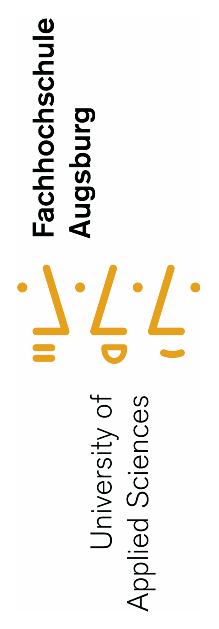
\includegraphics{fha_dpl_ct_logo} \\
				Studienrichtung
			 	& \\
				\vspace{0.5cm}
				Informatik
				& \\
				\vspace{2cm}
				\textbf{Benedikt Sauter} \\
				& \\
				USB-Stack for Embedded-Systems
				& \\
			\end{tabular}
		\end{flushright}
		\begin{tabular}{>{\LARGE}m{130mm}>{\scriptsize}m{50mm}}
			First Examiner: Prof. Dr. Hubert H�gl \newline
			Second Examiner: Prof. Dr. Gundolf Kiefer \newline
			Abgabe der Arbeit: 16.07.2007					
			& 
			Verfasser der Diplomarbeit: \newline
			Benedikt Sauter \newline
			Ketteng�sschen 6 \newline
			86152 Augsburg \newline
			sauter@ixbat.de \newline
			\newline
			Fakult�t \newline
			Informatik \newline
			Telefon: +49 821 5586-450 \newline
			Fax:       +49 821 5586-499 \newline
			\newline
			Fachhochschule Augsburg \newline
			University of Applied Sciences \newline
			Baumgartnerstra�e 16 \newline
			D 86161 Augsburg \newline
			\newline				
			Telefon +49 821 5586-0 \newline
			Fax +49 821 5586-222 \newline
			www.fh-augsburg.de \newline
			poststelle@fh-augsburg.de \newline
		\end{tabular}
\end{titlepage}


    %\maketitle
    \newpage

\thispagestyle{empty}
\markright{Erkl�rung}
\cleardoublepage
\vspace*{9cm}

Ich erkl�re hiermit, dass ich die Arbeit selbstst�ndig verfasst, noch nicht anderweitig f�r Pr�fungszwecke vorgelegt, keine anderen als die angegebenen Quellen oder Hilfsmittel benutzt sowie w�rtliche und sinngem��e Zitate als solche gekennzeichnet habe.\\

Augsburg, 16. Juli 2007\\
\vspace{2cm}

\vspace*{5mm}

Benedikt Sauter

%\parbox{7cm}{\hrulefill}\\
%\hspace*{2,5cm} \selectedthesisauthor

\cleardoublepage
\endinput

    \input{gfdl_short}


    
    % Inhalts-/Tabellen-/Abbildungsverzeichnis
    \tableofcontents
    
    % der eigentliche Text
    \mainmatter
    
    %Hier kommen die Kapitel hin
	\chapter{USB f�r Embedded Systeme}

\section{Einleitung}

\index{System on Chip}
\index{R232}
\index{Parallelport}
\index{Gameport}

\glqq{}Universal Serial Bus\grqq{} - kurz USB - ist speziell mit dem Ziel entwickelt worden,
die damals technisch veralteten Schnittstellen wie RS232, Parallelport, Gameport, usw. abzul�sen.
Mit USB sollten Kosten reduziert werden, der Anschluss und die Konfiguration
f�r den Nutzer vereinfacht und viele technische Probleme
von bereits existierenden Schnittstellen gel�st werden k�nnen.
\newline\newline
Zu Beginn von USB gab es nur Controller,
die fest im Chipsatz von Computern integriert waren. Es gab keine einzelnen
USB-Bausteine, mit denen man �ber einen
beliebigen Mikrocontroller USB-Ger�te h�tte ansteuern k�nnen.
Mittlerweile gibt es aber eine Vielzahl an USB-Bausteinen
f�r Embedded Systeme. Oft ist USB sogar schon ein fester Bestandteil
moderner \glqq{}System on Chip\grqq{}\footnote{\label{foot:1}Bei einem \glqq{}System on Chip\grqq{} sind im Silizium, neben dem Prozessor, RAM, ROM, Schnittstellenlogiken, uvm. integriert.} Einheiten.
Dadurch steht einem Embedded System mit einer USB-Schnittstelle nun die ganze Welt der USB-Peripherie zur Verf�gung.
\newline\newline
Ein Nachteil von USB ist jedoch,
dass die Spezifikation durch die vielen Anforderungen
zu einem sehr umfangreichen Text geworden ist.
Dadurch ist es schwierig, ohne tiefere Kenntnisse
eine Kommunikation mit einem Ger�t �ber USB
zu programmieren. Als Basis gibt es von vielen Anbietern
eigene kleine Bibliotheken, mit denen demonstriert wird,
wie der eingesetzte Baustein angewendet werden kann.
Doch oft stehen diese Bibliotheken unter nicht freien
Lizenzen und zeigen meist nur typische Standardaufgaben, wie z.B. die Anbindung
eines Massenspeichers oder �hnliches. Will man auf andere
Ger�te zugreifen, steht man wieder vor dem Problem,
dass man sich erst tief in die USB-Materie einarbeiten muss.
\newline\newline
Das Ziel der vorliegenden Diplomarbeit ist es, einen freien, portablen und
erweiterbaren USB-Host-Stack f�r Embedded Systeme zu entwerfen und zu implementieren.
Die Software soll als Basis f�r viele unterschiedliche USB-Host-Bausteine dienen.
Durch eine Aufteilung der Software in mehrere
Ebenen ist ein hoher Grad an Wiederverwendbarkeit gegeben. Wie dies im Einzelnen aussieht,
wird in den Kapiteln der Diplomarbeit wie folgt beschrieben.
\newline\newline
Begonnen wird in Kapitel 1 mit der Betrachtung der Aufgaben,
den Anforderungen und Einsatzgebieten von USB-Host-Stacks.
Im Anschluss werden in Kapitel 2 die Grundlagen des USB-Busses
beschrieben. Dies soll dem Leser helfen, besser zu verstehen,
was beim Entwurf des USB-Host-Stacks zu beachten ist.
Aufbauend darauf werden in Kapitel 3 die Komponenten und ihre
Aufgaben im USB-Host-Stack diskutiert. Die Implementierung der 
einzelnen Ebenen des USB-Host-Stacks werden anschliessend in 
Kapitel 4, 5 und 6 beschrieben. In Kapitel 7 wird
die im Rahmen der Diplomarbeit entworfenen Testplatine vorgestellt.
Zuletzt wird in Kapitel 8 ein Ausblick auf zuk�nftige Arbeiten
und ein Fazit �ber die getane Arbeit gegeben.

%\chapter{USB f�r Embedded Systeme}

%Das folgende Kapitel soll einen groben �berblick �ber die wesentlichen
%Aufgaben, Anforderungen und Einsatzgebiete von USB-Host-Stacks geben.

\section{Aufgaben eines USB-Host-Stacks}
\index{USB-Host-Stack}
\index{USB-Stack}
\index{Treiberstack}
\index{Aufgaben des USB-Stacks}

Ein USB-Host-Stack\footnote{\label{foot:1} Ein Stack ist in der Informatik eine konzeptuelle Architektur von Software, die f�r die Daten�bertragung zust�ndig ist.} steuert als einzige Softwarekomponente des USB-Busses
alle Hardwarekomponenten. Oft wird diese Software auch USB-Host-Stack, USB-Host, USB-Subsystem oder
USB-Stack genannt. In dieser Diplomarbeit wird die Softwarekomponente als USB-Stack bezeichnet.
\newline

\index{USB-Bus}
Der USB-Bus ist ein h�chst flexibler, erweiterbarer und aufw�ndiger Bus.
Jederzeit ist es m�glich, neue Ger�te w�hrend der Laufzeit hinzuzuf�gen und zu entfernen.
Parallel dazu k�nnen entweder viele verschiedene �bertragungen stattfinden, oder
Ger�te m�ssen entsprechend ihrer Aktivit�ten in den Standby Zustand versetzt
und bei Bedarf wieder aktiviert werden. Alle diese Aufgaben m�ssen
rechtzeitig und geordnet vom USB-Stack erledigt werden.
\newline

Um unabh�ngig vom
eingesetzten Bausteinen einen hohen Grad an Wiederverwendbarkeit
zu erreichen, ist der USB-Stack in mehrere
Treiber\footnote{\label{foot:1} In der USB-Spezifikation werden alle Teilmodule, inklusive der Verwaltungseinheiten, als Treiber
bezeichnet.} aufgeteilt. Daten
werden von Treiber zu Treiber weitergereicht, daher auch der Name USB-Stack (deutsch: Stapel).
Der USB-Stack muss Funktionen anbieten, um die Treiber in den Datenfluss integrieren zu k�nnen.
\newline
\newline
Die Hauptarbeit des USB-Stacks besteht in der Verwaltung und Steuerung der Treiber und der angeschlossenen Ger�te.
Im Einzelnen fallen darunter die folgenden Aufgaben:

\begin{itemize}
\item das Erkennen von neuen Ger�ten
\item die Generierung von Standardanfragen
\item die Verwaltung des Datenflusses
\item die Bandbreitenverteilung
\item das Laden und Entladen von Treibern
\item die Fehlerpr�fung
\item die Stromversorgung und das \glqq{}Power Management\grqq{}
\item der Datenaustausch mit den Peripherieger�ten
\end{itemize}


\section{Spezielle Anforderungen an Embedded Systeme}
\index{Programmiersprache C}
\index{Portierbarkeit}

Urspr�nglich wurde USB so geplant, dass der USB-Stack auf einem Computer
mit einem modernen Prozessor und ausreichend Arbeitsspeicher arbeitet. In einem
PC-USB-Stack wird daher immer der komplette Status des Busses, mit allen M�glichkeiten
der Konfigurationen und Einstellungen f�r jedes USB-Ger�t, in einer 
internen Datenstruktur im Arbeitsspeicher gehalten. 
In kleinen Embedded Systemen ist meist nur wenig Arbeitsspeicher vorhanden, was bedeutet,
dass hier viel Platz eingespart werden muss.
\newline\newline
Wie beim Arbeitsspeicher, trifft dies auch auf die Programmgr��e zu.
W�rden alle Funktionen wie die eines USB-Stacks f�r Computer-Betriebssysteme realisiert werden, 
so h�tte das eigentliche Programm auf sehr kleinen Embedded Systemen wahrscheinlich keinen Platz mehr.
Daher muss sich der Stack flexibel mit den nur absolut notwendigen
Komponenten zusammenstellen lassen k�nnen, um ihn auf vielen verschiedenen Embedded Systemen
einsetzbar zu machen.
\newline\newline
F�r die Portierbarkeit spielt nicht nur die Anforderung von Arbeitsspeicher
und Programmcode eine wichtige Rolle, sondern auch die
Verbreitung und Unterst�tzung der Programmiersprache, in der der Stack geschrieben
ist. Aus diesem Grund wurde der USB-Stack in ANSI C geschrieben.

\section{Einsatzgebiete}

Der Einsatz von USB in Embedded Systemen gewinnt zunehmend an Bedeutung.
Im Bereich der USB-Ger�te finden sich sehr viele L�sungen, die fr�her oft
als Spezialentwicklungen �ber verschiedenste Busse bzw. Ports mit
eigenen Steckverbindungen realisiert worden sind. Allerdings ist dies durch den
gro�en USB-Markt nicht mehr n�tig. Es k�nnen erhebliche Entwicklungskosten
eingespart werden, wenn fertige USB-Ger�te wie Kameras, Festspeicher, Festplatten, Soundkarten, Netzwerkkarten, etc.
in Embedded Systeme eingesetzt werden.

\section{Markt�bersicht}

\index{kommerzielle USB-Stacks}
\index{Markt�bersicht}
\index{USB-Stacks}

Wie in der folgenden Markt�bersicht zu sehen ist, gibt es bereits einige USB-Stacks f�r Embedded Systeme.
Bei der Recherche wurde jedoch kein freier USB-Stack gefunden. F�r kommerzielle
Versionen ist es keine Seltenheit, dass Lizenzen bis zu einigen tausend Euro kosten.
\newline\newline

\textbf{USBware\texttrademark{} von Jungo Ltd. (http://www.jungo.com/)} \newline
Mit USBware\texttrademark{} bietet Jungo einen vollst�ndigen
USB-Stack an, f�r den es eine Vielzahl von Ger�te- und Host-Controller-Treibern gibt.
Es werden alle
Transferarten und Geschwindigkeitsklassen unterst�tzt.
Der Stack ist komplett in C geschrieben und l�sst sich mit jedem 32-Bit C-Compiler
�bersetzen. 
\newline\newline

\textbf{USB-Software-Stack von Mentor Graphics Corp. (http://www.mentor.com/)} \newline
Mentor Graphics bietet IP Modelle\footnote{\label{foot:1} von engl. \textit{Intellectual Property} $-$ \glqq{}Geistiges Eigentum\grqq{}, elektronische Designs von Schaltungen.} f�r USB-Host und -Device-Controller
an. F�r diese Modelle hat Mentor Graphics das Produkt \glqq{}USB Software Stack\grqq{} entwickelt. Der Stack stellt alle Funktionen eines USB 2.0 Hosts bereit.
Au�erdem wird der OTG-Standard\footnote{\label{foot:1} USB-Standard f�r die Punkt-zu-Punkt Vernetzung von USB-Ger�ten.} ebenfalls unterst�tzt.
Der Quelltext ist in C geschrieben und daher auf viele Prozessoren portierbar.
\newline\newline

\textbf{$�$C$/$USB-Host von Micrium (http://www.micrium.com/)} \newline
Der USB-Stack von Micrium unterst�tzt den kompletten USB 2.0 Standard. F�r die Kommunikation
mit USB-Ger�ten werden Klassentreiber f�r Massenspeicher, HID-Ger�te\footnote{\label{foot:3} Human-Interface-Devices, Eingabeger�te f�r den Computer.} 
und CDC-Ger�te-Treiber\footnote{\label{foot:4} Ger�teklasse f�r Kommunikationsger�te wie Netzwerkkarten, RS232 Schnittstellen, etc.} angeboten.
Der Stack kann mit verschiedenen Host-Controllern arbeiten.
\newline\newline

\textbf{Vinculum von Future Technology Devices International (http://www.vinculum.com/)} \newline
FTDI bietet mit dem Produkt Vinculum einen programmierbaren Controller an, der ohne viel
Aufwand mit fertigen Bin�rprogrammen programmiert werden kann und auf diese Weise 
USB mit bekannten Schnittstellen wie RS232, SPI, etc. verbindet.
Die Bin�rprogramme k�nnen, mit einem eigens daf�r entwickelten Programm von FTDI in den Vinculum Chip geladen werden.
\newline\newline

\textbf{Thesycon (http://www.thesycon.de/)} \newline
Mit dem Produkt \glqq{}Embedded USB Host Stack\grqq{} bietet die Firma Thesycon einen
nach eigenen Angaben industrietauglichen, standardkonformen USB-Host-Stack an.
Aktuell werden die Host-Controller NXP ISP1362, NXP1160/61 und OHCI unterst�tzt.
F�r die USB-Ger�te-Kommunikation gibt es Klassentreiber f�r HID, Massenspeicher
und Drucker.

	
\chapter{Grundlagen}

Eine Entwicklung von USB-Programmen ohne ein tiefergehendes Verst�ndnis
der Funktionsweise des USB-Busses ist nur schwer m�glich.
Daher werden in diesem Kapitel einige USB-Konzepte und -Hintergr�nde kurz erl�utert. Die
Beschreibung ist im Wesentlichen an die USB-Spezifikation \cite{usb_spec} angelehnt.
Um einen tieferen Einblick in USB zu bekommen, k�nnen die B�cher \cite{kelm2001} und \cite{axelson2001}
empfohlen werden.


\section{Die USB-Geschichte}
\index{Geschichte}

USB wurde als Standardschnittstelle f�r den Computer entworfen. 
Die Entwicklung ist von den Firmen Compaq, Intel, Microsoft und NEC
im Rahmen der daf�r neu gegr�ndeten Organisation
\glqq{}USB Implementers Forum Inc.\grqq{} \cite{usborg} durchgef�hrt worden.
\newline\newline
Das Besondere an dieser Organisation ist, dass alle Spezifikationen
kostenlos im Internet erh�ltlich sind. Begonnen hat die Freigabe damit,
dass im Januar 1996 die erste Version USB 1.0 nach einer mehrj�hrigen
Entwicklung ver�ffentlicht wurde. Im September 1998 folgte
die Version 1.1, welche einige Fehler und Unklarheiten aus der vorherigen Version behob.
\newline\newline
Der n�chste gro�e Schritt f�r USB war die Version 2.0.
Das Hauptziel bestand darin, eine Erh�hung der Datenrate und eine vollst�ndige R�ckw�rtskompabilit�t  
zu den vorherigen USB-Versionen. Die USB 2.0 Spezifikation wurde im April 2000 ver�ffentlicht.

\section{Ziele des USB-Standards}

USB sollte als Nachfolger f�r bestehende Computerschnittstellen
entwickelt werden. Aus diesem Grund mussten viele Faktoren und Gegebenheiten
bei dem Entwurf von USB bedacht werden. 
\newline\newline
Die Bedienung f�r den Nutzer sollte durch \glqq{}Hot Plug and Play\grqq{}, dem
einheitlichen Steckerverbindungssystem und der integrierten Stromversorgung f�r Ger�te,
stark vereinfacht werden. Zur Bedienung geh�rte auch die Konfiguration
und Installation, welche f�r die Nutzer oftmals eine gro�e H�rde bedeuteten.
F�r Standardger�te wie Maus, Tastatur, Drucker, etc., wurden deshalb USB-Klassen definiert.
Betriebssysteme k�nnen solche USB-Klassen-Ger�te erkennen
und automatisch Standardtreiber f�r sie laden \cite{usb_class}.
\newline\newline
Es ergaben sich nicht nur Vorteile f�r den Nutzer, sondern auch viele Vorteile
aus Sicht der Hardware-, Firmware- und Softwareentwickler.
USB-Ger�te ben�tigen keine eigenen Systemressourcen wie I/O Adressen oder
Interruptsignale. Der USB-Bus ben�tigt die Ressourcen lediglich einmal f�r den sogenannten
Host-Controller. 
Durch Hubs entfallen ebenfalls
Engp�sse wie bei konventionellen, parallelen oder seriellen Schnittstellen,
bei denen meist nur der Anschluss eines Ger�tes erlaubt ist.
\newline\newline
Mit USB sollten nicht nur neue Ger�te erstellt werden, sondern auch bestehende Schnittstellen
ersetzt werden. Dass dies erfolgreich war, sieht man an den Beispielen von RS-232, Gameport, der Centronics-Schnittstelle und der PS/2-Schnittstelle
f�r Tastaturen bzw. M�use, die schon oft an neuen Computern nicht mehr vorhanden sind.

Die Eigenschaften f�r die USB-Schnittstelle wurden vor ca. zehn Jahren definiert und sie sind immer noch aktuell. Das wiederum zeigt,
dass USB noch sehr viel Potenzial im Computer und in Embedded Systemen hat.

\section{Die USB-Topologie} \label{kap:topologie}

\index{Topologie}
\index{Physikalische Struktur}
\index{Logische Struktur}

Topologisch existieren f�r den USB-Bus zwei Modelle. Das physikalische,
welches die Struktur als Baum darstellt (Abbildung \ref{bus}), und das logische, welches
die Struktur als Stern-Architektur (Abbildung \ref{stern}) abbildet.
\newline\newline
Beim physikalischen Modell bildet der Host den Stamm des Baumes. Die Verzweigungsknoten stellen Hubs dar
und die �ste entsprechen den Kabeln. Am Ende der �ste befinden sich die Blattknoten,
welche die Endger�te repr�sentieren.

\begin{figure}[h]
{
\centering
\includegraphics[width=10cm]{images/bus}
\caption{Physikalische Baumstruktur von USB}
\label{bus}
}
\end{figure}

Im logischen Modell bildet der Host den zentralen Mittelpunkt, an dem jedes
Endger�t direkt angeschlossen ist. 
Da es sich bei USB um einen
\glqq{}Single Master Bus\grqq\footnote{\label{foot:1}\glqq{}Single Master Bus\grqq{} bedeutet, es gibt nur einen Teilnehmer auf dem Bus, der jeglichen Datenverkehr initiieren darf.}
handelt, muss der Host jegliche Kommunikation initiieren und steuern.

\begin{figure}[h]
{
\centering
\includegraphics[width=10cm]{images/stern}
\caption{Logische Stern-Architektur von USB}
\label{stern}
}
\end{figure}

Ausgehend von der Topologie werden im n�chsten Abschnitt
die einzelnen Hardwarekomponenten beschrieben.

\section{�bersicht der USB-Komponenten}

\index{USB-Komponenten}

Grundlage f�r den USB-Bus bilden die einzelnen Hardwarekomponenten (siehe Abbildung \ref{komponenten}),
welche im Verbund die Kommunikation erst erm�glichen.
Im Folgenden werden die wichtigsten Komponenten kurz vorgestellt.

\begin{figure}[h]
{
\centering
\includegraphics[width=8cm]{images/komponenten}
\caption{�bersicht der USB-Komponenten}
\label{komponenten}
}
\end{figure}

\index{USB-Function}

Der Host-Controller ist f�r die Codierung, �bertragung und dem Empfang der Datenstr�me
von und zu den Endger�ten zust�ndig. 
\newline\newline
Ein USB-Hub ist ein USB-Ger�t genauso wie beispielsweise eine Maus, ein Drucker etc.
Die Aufgabe des Hubs besteht darin, alle ankommenden USB-Signale an zus�tzliche Ports zum Anschluss von weiteren Ger�ten weiterzuleiten.
Hubs k�nnen Strom aus dem Bus beziehen, oder selbst Strom in den USB-Bus einspeisen.
\newline\newline
Der Root-Hub ist ein USB-Hub, der sich direkt hinter dem Host-Controller befindet. 
Der gr��te Unterschied zu einem \glqq{}echten\grqq{} USB-Hub ist der, dass die Status�nderungen an den Ports
des Hubs nicht �ber eine USB-Verbindung abgefragt werden, sondern �ber interne Signale (Interrupts) und Register
signalisiert werden.
\newline\newline
Das Endger�t, welches in der Spezifikation als \glqq{}Function\grqq{} bezeichnet wird,
ist das eigentliche Peripherieger�t und dient meist als Drucker, Scanner, Festspeicher, Kamera, etc.
\newline\newline
Die Aufgaben und die Struktur von USB-Endger�ten werden im n�chsten Abschnitt n�her beschrieben.


%**********************************************************************

\section{Aufgaben und Struktur von USB-Ger�ten}
\index{USB-Ger�t}

Zu den Aufgaben, f�r die ein Ger�t gebaut worden ist, wie z.B. eine Maus f�r die Ermittlung von X-Y Koordinaten,
eine Soundkarte f�r die Ausgabe von Audio-Dateien, etc., muss das Ger�t noch zus�tzliche USB-Verwaltungsarbeiten unterst�tzen.
\newline\newline
\textbf{Erkennen einer Kommunikation: }
Das USB-Ger�t muss erkennen, wenn Daten vom Host angefordert werden.
\newline\newline
\textbf{Antworten auf Standardanfragen: }
�ber die sogenannten Standardanfragen kann ein Betriebssystem, Treiber, Programm, etc.
Informationen direkt beim Ger�t selbst abholen. Mehr dazu in Kapitel \ref{kap:anfragen} auf Seite \pageref{kap:anfragen}. 
\newline\newline
\textbf{Fehlerpr�fung: }
Die ankommenden Datenstr�me m�ssen auf Fehler �berpr�ft und gegebenenfalls 
neu angefordert werden.
\newline\newline
\textbf{Power-Management: }
Ein Ger�t kann sich in verschiedenen Stromverbrauchszust�nden befinden. Um nicht unn�tig
Strom zu verbrauchen, kann zum Beispiel der Host ein Ger�t oder ein Ger�t sich selbst in den Standby-Modus versetzen.
\newline\newline
\textbf{Datenaustausch mit dem Host: }
F�r die Kommunikation mit dem Host m�ssen M�glichkeiten (Pufferspeicher, Status-Register, etc.)
bereitstehen.
\newline\newline
Da diese Aufgaben sehr aufw�ndig sind, gibt es daf�r spezielle USB-Ger�te-Bausteine (engl. \glqq{}USB-Device-Controller\grqq{}).
Mit welchem Anteil der USB-Controller das USB-Protokoll 
per Hardware ausf�hrt, h�ngt ganz vom Hersteller und dessen Zielgruppe
ab. Es gibt eine gro�e Vielfalt an USB-Bausteinen (siehe Tabelle \ref{usb_bausteine}) auf dem Markt.
Grunds�tzlich muss ein USB-Ger�te-Baustein aber mindestens
die folgenden f�nf typischen Teilkomponenten (Abbildung \ref{function}) enthalten.
\newline

\index{SIE}
\index{Transceiver}
\index{FIFO}
\index{Mikrocontroller}
\index{State-Machine}
\index{USBN9604}
\index{AN2131}
\index{MAX34xx}

\begin{figure}[h]
{
\centering
\includegraphics[width=13cm]{images/function}
\caption{Architektur eines USB-Ger�te-Bausteins}
\label{function}
}
\end{figure}

\begin{description}
\item [USB-I/O-Treiber (\glqq{}Transceiver\grqq{}):]
Der USB-I/O-Treiber stellt die physikalische Verbindung zum USB-Bus her. Bis auf ein
paar Ausnahmen muss der USB-I/O-Treiber die seriellen Signale von der \glqq{}SIE\grqq{} (\glqq{}Serial Interface Engine\grqq{})
differentiell �bertragen und empfangene differentielle Signale wieder in ein serielles Signal zur�ckwandeln.
Auf dem Bus werden bestimmte Signale wie EOP (\glqq{}End-Of-Packet\grqq{}), USB-Reset, etc. \cite{kelm2001} nicht differentiell �bertragen.
Diese Zust�nde muss der Treiber erkennen k�nnen. Mehr dazu in Kapitel \ref{kap:signal} auf Seite \pageref{kap:signal}.

\item [Serial Interface Engine (\glqq{}SIE\grqq{}):]
Die SIE ist f�r die Decodierung und Codierung des seriellen Datenstroms zust�ndig. Mehr dazu in Kapitel \ref{kap:signal} auf Seite \pageref{kap:signal}.

\item [SIE/FIFO-Control-Einheit:]
Die SIE/FIFO-Control-Einheit ist ein endlicher Automat der die SIE, die FIFOS und den USB-Treiber entsprechend
den ankommenden Anfragen vom Host ansteuert.

\item [FIFO(s):]
F�r die ankommenden und abgehenden Daten werden FIFO-Speicher als Zwischenpuffer eingesetzt. Sie dienen
meist dem Embedded System als Schnittstelle f�r die Daten�bertragung.

\item [Mikrocontroller oder State-Machine:]
Um die Standardanfragen beantworten und weitere Verwaltungsaufgaben erledigen zu k�nnen, wird ein Mikrocontroller
oder Zustandsautomat ben�tigt.
\end{description}

\begin{table}[h]
\center
\begin{tabular}{|l|c|c|c|c|c|}
\hline
\rowcolor{Gray}[0.9\tabcolsep]
Baustein &  Transceiver & SIE & FIFOs & State Machine & interne CPU\\ \hline
USBN9604 \cite{national} &  x & x & x & x & \\ \hline
AN2131 \cite{cypress} &  x & x & x & x & x\\ \hline
MAX34xx \cite{maxim} &  x &  &  &  & \\ \hline
\end{tabular}
\caption{USB-Bausteine}
\label{usb_bausteine}
\end{table}



Im n�chsten Abschnitt
wird der Datenfluss zwischen dem USB-Host-Controller und dem USB-Ger�te-Baustein beschrieben.


\section{Datenfluss auf dem USB-Bus}

\index{NRZI}
\index{DPLL}
\index{Bitstuffer}

Wie bereits in Kapitel \ref{kap:topologie} erw�hnt, handelt es sich bei USB um einen
\glqq{}Single Master Bus\grqq{}. Das hei�t, dass nur der Host eine Kommunikation
initiieren kann. USB-Ger�te d�rfen ohne Anforderung durch den Host 
nicht senden. 
\newline\newline
W�hrend einer Kommunikation werden auf dem Bus Datenpakete �bertragen.
Mit speziellen Datenpaketen kann eine Adresse f�r den Empf�nger des
folgenden Datenstroms angegeben werden. Die Daten werden dann dennoch im Broadcast-Modus
an alle Teilnehmer im Netz geschickt, und nur das Ger�t, das seine Adresse
im Paket entdeckt, nimmt die Daten an und antwortet.
\newline\newline
In der USB-Spezifikation wird von \glqq{}Downstream\grqq{} gesprochen,
wenn der Host Daten sendet und von \glqq{}Upstream\grqq{},
wenn Daten von einem Ger�t zum Host �bermittelt werden.


\section{Signalleitungen/Datenkodierung} \label{kap:signal}
\index{Signalleitungen}
\index{Datenkodierung}
Ein USB-Kabel (siehe Abbildung \ref{kabel} auf Seite \pageref{kabel}) besteht aus vier Leitungen.
D+ und D-, welche bis auf ein paar Ausnahmen differentiell getrieben werden,
dienen der Daten�bertragung. Vcc und GND sind f�r die Stromversorgung der Endger�te da. \cite{kelm2001}
\begin{figure}[h]
{
\centering
\includegraphics[width=15cm]{images/kabel}
\caption{Querschnitt USB-Kabel}
\label{kabel}
}
\end{figure}
\newline\newline
Auf den Datenleitungen werden ausschlie�lich codierte Daten �bertragen. Das hat zum Ersten den Grund,
dass eine erh�hte Datensicherheit f�r die �bertragung gew�hrleistet ist. Zum Zweiten
kann der Empf�nger den Takt, mit denen die Daten versendet worden sind anhand der empfangenen Daten zur�ckgewinnen.
Technisch l�uft die Codierung wie in Abbildung \ref{nrzi} dargestellt ab.
\newline\newline
Die Daten werden �ber ein Schieberegister serialisiert und anschlie�end
in ein \glqq{}Bitstuffer\grqq{} geschoben. Der \glqq{}Bitstuffer\grqq{} f�gt nach jedem sechsten Bit
eine Null ein. Dies wird f�r den n�chsten Schritt der NRZI-Codierung ben�tigt.
NRZI steht f�r Non-Return-to-Zero-Inverted und ist ein oft verwendetes Codierungsverfahren.
Wird im Eingansdatenstrom eine 0 entdeckt, so findet ein Polarit�tswechsel statt, bei 
einer 1 bleibt der Datenstrom unver�ndert. Der Empf�nger kann sich so mit einer DPLL \cite{dpll}
synchronisieren und den Takt dadurch zur�ckgewinnen.

\begin{figure}[h]
{
\centering
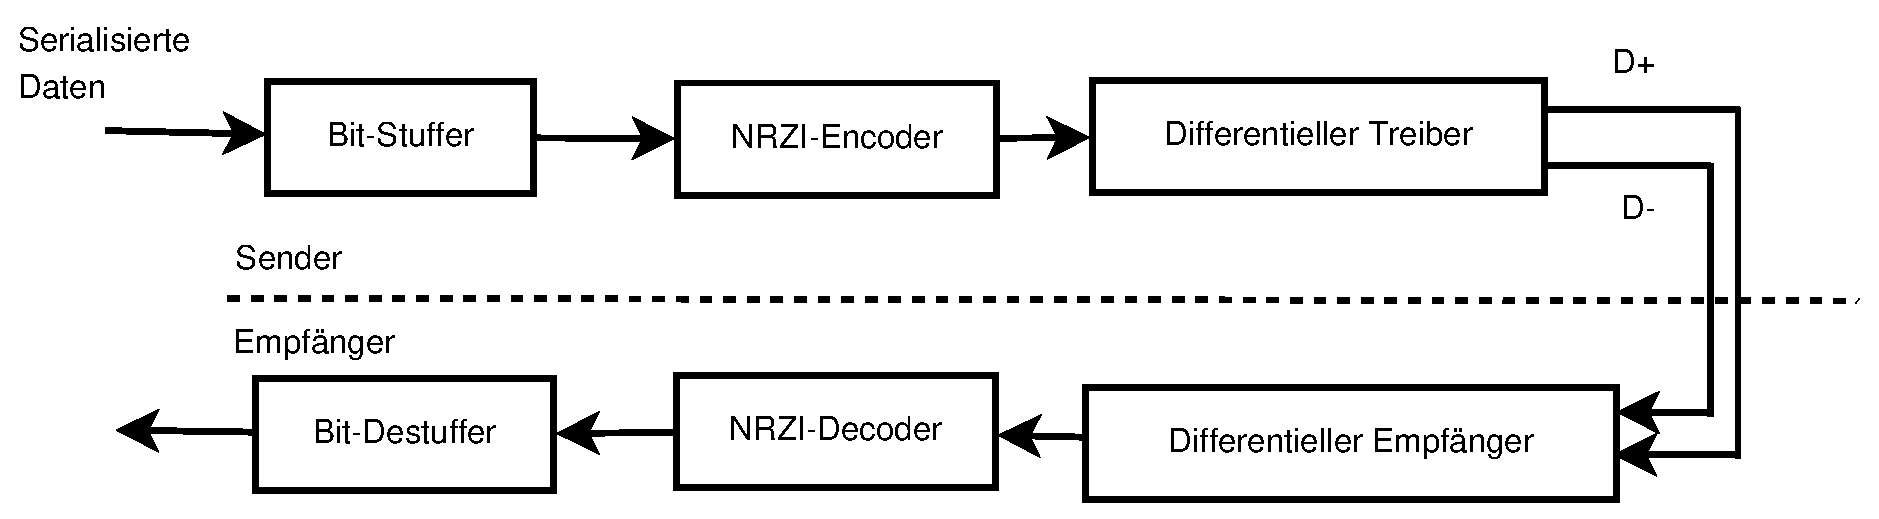
\includegraphics[width=15cm]{images/nrzi}
\caption{Datenfluss der Low-Level-Datencodierung}
\label{nrzi}
}
\end{figure}


\section{Paketformate und Zeitrahmen} \label{kap:pakzei}

Wie bereits erw�hnt, werden auf dem USB-Bus einzelne Pakete (\glqq{}USB-Packets\grqq{}) �bertragen.
In der Tabelle \ref{usb_pid} sind alle verschiedenen Typen von USB-Paketen aufgelistet.

\begin{table}[h]
\center
\begin{tabular}{|l|l|l|}
\hline
\rowcolor{Gray}[0.9\tabcolsep]
PID Name & Gruppe & Beschreibung\\ \hline
SOF & Token-Paket & Framesignalisierung (jede ms) f�r Ger�te\\ \hline
SETUP & Token-Paket & Ank�ndigung einer Standardanfrage\\ \hline
IN & Token-Paket & Host will Daten empfangen\\ \hline
OUT & Token-Paket & Host will Daten senden\\ \hline
DATA0 & Data-Paket & Datenpaket ohne gesetztem Togl-Bit\\ \hline
DATA1 & Data-Paket & Datenpaket mit gesetztem Togl-Bit\\ \hline
ACK & Handshake-Paket & Best�tigungspaket\\ \hline
NAK & Handshake-Paket & �bertragung fehlerhaft - �bertragung wiederholen\\ \hline
STALL & Handshake-Paket & gr�sserer Fehler beim Empfangen - Abbruch\\ \hline
PRE & Special-Paket & k�ndigt Datenempfang bei Low-Speed an\\ \hline
\end{tabular}
\caption{Codierung der USB-Token-Pakete}
\label{usb_pid}
\end{table}

Die Grundstruktur eines USB-Pakets sieht wie in Abbildung \ref{packet} aus.
Jedes Paket beginnt mit
einem 8-Bit langen \textbf{SYNC}-Feld. Dieses
besteht aus 7 Nullen und einer Eins am Ende. Die aufeinander folgenden Nullen
bewirken bei der NRZI-Codierung einen regelm��igen Polarit�tswechsel.
Im Anschluss folgt das 8-Bit breite \textbf{PID}-Feld. Dort steht ein Paket-Typ aus der Tabelle \ref{usb_pid}.
Nach dem PID-Feld folgen abh�ngig vom Paket-Typ paketspezifische Daten. Die \textbf{CRC5}-Pr�fsumme
dient dem Kommunikationspartner zum �berpr�fen der Daten auf Korrektheit, mit \textbf{EOP} (\glqq{}End-of-Paket\grqq{})
wird das Ende des Paketes markiert.

%sync, paket, parameter, crc5, eop
\begin{figure}[h]
{
\centering
\includegraphics[width=15cm]{images/packet}
\caption{Aufbau der \glqq{}USB-Pakete\grqq{}}
\label{packet}
}
\end{figure}


\index{SNYC}
\index{CRC5}
\index{EOP}
\index{PID}


Der Host versendet jede Millisekunde ein SOF-Paket (\glqq{}Start-of-Frame\grqq{}). Dieses SOF-Paket teilt
den gesamten Bus in einzelne Zeitabschnitte (sogenannte \glqq{}Frames\grqq{}) ein.
Full-Speed und High-Speed Ger�te k�nnen �ber dieses SOF-Paket die Frame-Einteilung erkennen.
Low-Speed Ger�te m�ssen aber wegen ihrer geringen Speicher- und Rechenkapazit�ten vor SOF-Paketen gesch�tzt werden,
da sie sonst ausschlie�lich mit dem Decodieren der SOF-Pakete besch�ftigt w�ren und keine
anderen Pakete mehr annehmen k�nnten. Daher m�ssen Hubs an den Ports, an denen sich Low-Speed Ger�te
befinden, die SOF-Pakete wegfiltern.
Dass Low-Speed Ger�te dennoch die Einteilung der Frames auf dem USB-Bus erkennen, muss
der letzte Hub oder Root-Hub vor dem Ger�t EOP-Signale auf dem Bus erzeugen.
Ein EOP-Signal ist eines von drei speziellen Signalen (siehe Tabelle \ref{speziellsignal}), die nicht differentiell
auf dem USB-Bus �bertragen werden, und ist daher mit viel geringerem Aufwand dekodierbar.
\newline\newline
Zur�ck zu den Aufgaben des SOF-Pakets. Ein SOF-Paket hat noch einen zweiten Nutzen, es dient als Ank�ndigung
f�r weitere Daten-Pakete. Denn nur direkt nach einem SOF-Paket k�nnen Daten-Pakete gesendet werden (siehe Abbildung \ref{zeittakt}).
\begin{figure}[h]
{
\centering
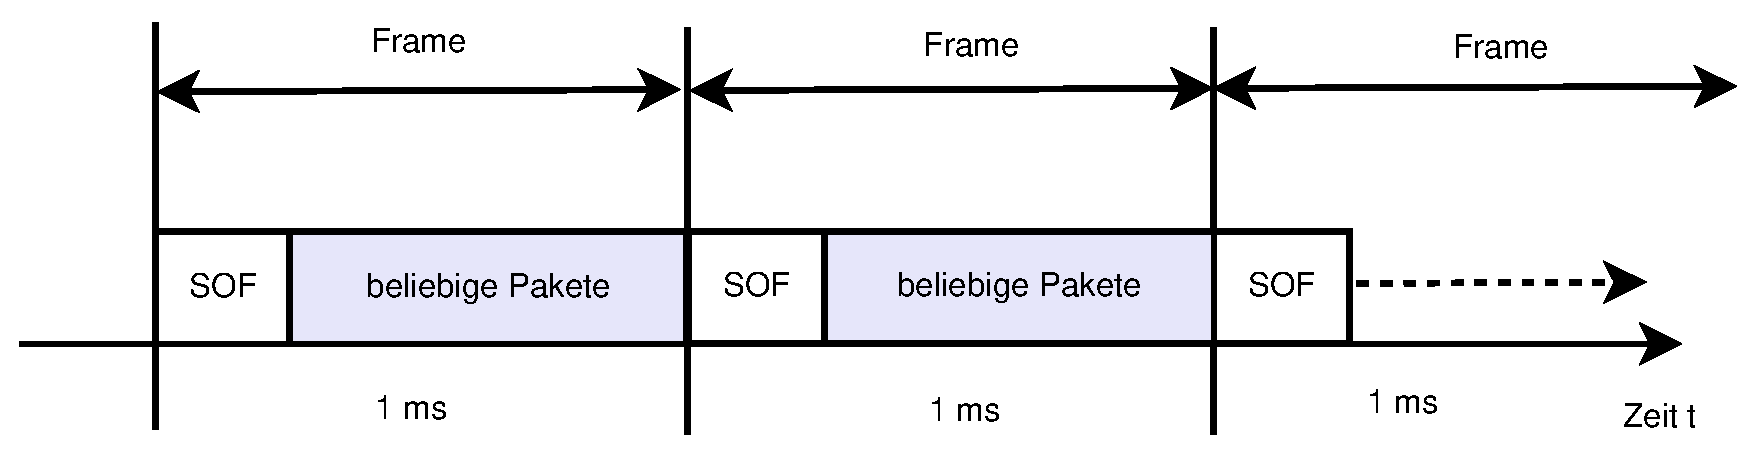
\includegraphics[width=15cm]{images/zeittakt}
\caption{Zeittakt des USB}
\label{zeittakt}
}
\end{figure}
Da Low-Speed Ger�te jedoch keine SOF-Pakete empfangen k�nnen, wird ein Low-Speed Datentransfer mit einem
PRE-Paket (\glqq{}Spezial Token\grqq{}) angek�ndigt.

Im Datenbereich eines SETUP-, IN- oder OUT-Pakets ist eine Ger�teadresse und ein Endpunkt angeben.
Danach k�nnen Daten, verpackt in DATA0- und DATA1-Pakete, f�r das angegebene Ger�t folgen.
Die restlichen Pakete ACK, NAK und STALL dienen zur Flusskontrolle und damit
indirekt zur Umsetzung der verschiedenen Transferarten, die �ber USB angeboten werden.

\index{ACK}
\index{NAK}
\index{STALL}
\index{DATA0,DATA1}

\begin{table}[h]
\center
\begin{tabular}{|l|l|}
\hline
\rowcolor{Gray}[0.9\tabcolsep]
Signal & Beschreibung \\ \hline 
EOP & Signalisiert Ende eines Paketes \\ \hline 
Reset & USB-Ger�t in Reset Zustand zwingen \\ \hline 
Connect & Neues USB-Ger�t wurde angeschlossen\\ \hline
Disconnect & USB-Ger�t wurde entfernt\\ \hline
\end{tabular} \caption{Nicht-differentielle Signale} \label{speziellsignal}
\end{table}

\index{Nicht-differentiellen Signale}

\index{Transferarten}
\index{Control-Transfer}
\index{Bulk-Transfer}
\index{Interrupt-Transfer}
\index{Isochronous-Transfer}

\section{Transferarten}
Um die unterschiedlichen Ger�te und Anwendungen zu unterst�tzen, sind in der USB-Spezifikation
vier verschiedene Transferarten definiert:
\begin{description}
\item[Bulk-Transfer]
Der Bulk-Transfer wird am meisten genutzt. Es k�nnen gro�e und zeitunkritische Datenmengen �bertragen werden. F�r den Bulk-Transfer ist keine feste Bandbreite auf dem Bus reserviert. Er wird nach allen zeitkristischen Transfers durchgef�hrt. Zus�tzlich �berpr�ft dieser Transfer stets die Korrektheit der �bertragenen Daten. 
\item[Interrupt-Transfer]
Diese �bertragungsart darf nicht w�rtlich genommen werden, denn USB ist ein Single Master Bus. Das bedeutet, nur der Master darf jegliche Kommunikation initiieren. Kein Ger�t kann sich beim Master selbst anmelden und ihm mitteilen, dass es Daten �bertragen will. Der Master muss zyklisch alle Ger�te nach neuen Daten abfragen. Im Grunde ist der Interrupt-Transfer nichts anderes als der Bulk-Transfer mit dem Unterschied, dass die Interrupt-Endpunkte eine h�here Priorit�t und daher mehr Bandbreite bekommen. Auf diese Weise kann der Master immer zu dem gew�nschten Zeitpunkt auf das Ger�t zugreifen, selbst dann, wenn gerade viel Datenverkehr auf dem Bus ist.
\item[Isochronous-Transfer]
Mit dem Isochronen Modus k�nnen Daten �bertragen werden, die eine konstante Bandbreite erfordern. Typische Anwendungsbeispiele sind die �bertragung von Audio- oder Videosignalen. Geht hier ein Bit oder Byte verloren, �u�ert sich das im Signal nur mit einem \glqq{}Knacken\grqq{} oder \glqq{}Rauschen\grqq{}. W�rden die Daten aber verz�gert ankommen, w�re die Sprache oder das Bild v�llig verzerrt und daher unbrauchbar.
Es muss ebenso wie beim Interrupt-Transfer das Pollingintervall angegeben werden.
\item[Control-Transfer]
Der Control-Transfer ist an dieser Stelle noch zu erw�hnen. Er wird ausschliesslich beim sogenannten Endpunkt 0 f�r
Standard-, Hersteller-, und Klassenanfragen eingesetzt. F�r andere Endpunkte
kann dieser Transfer nicht verwendet werden. Mehr dazu in Kapitel \ref{kap:anfragen} auf Seite \pageref{kap:anfragen}.
\end{description}

%USB unterscheidet zwischen zwei verschiedenen Pipe-Konzepten: Message-Pipes und Stream-Pipes.
%Daten die �ber eine Message Pipe �bertragen werden, besitzen eine fest vorgegebene Datenstruktur
%durch die USB-Spezifikation. Mit Stream-Pipes k�nnen frei definierte Datenstr�me �bertragen werden.
%Da nur die Anfragen f�r Endpunkt 0 in der USB Spezifikation festgelet sind, ist dies auch der
%einzige Endpunkt der mit dem Message-Pipe Konzept arbeitet. Ebenfalls kann eine Message-Pipe
%nur �ber einen Control-Transfer Endpunkt realisiert werden, welcher wiederrum nur f�r Endpunkt 0 zugelassen ist.
%Daher arbeitet man bei der �bertragung von eigenen Daten immer mit Stream-Pipes die mittels
%Bulk-, Isochronous- oder Interrupt-Transfers realisiert werden.


\section{Endpunkte f�r die Datenkommunikation}

\index{Endpunkte}
\index{Pipe}

Die Datenkommunikation des USB geschieht �ber die sogenannten Endpunkte.
Jedes USB-Ger�t kann bis zu 16 Endpunkte haben.
Physikalisch gesehen ist ein Endpunkt ein FIFO mit einer festgelegten Tiefe, �ber
den Daten gesendet oder empfangen werden k�nnen.
Will ein Anwendungsprogramm oder Treiber Daten empfangen oder senden,
so kann dies �ber eine Anfrage, die die Ger�teadresse, 
den Endpunkt inklusive der gew�nschten Richtung und die Transferart enth�lt, geschehen.
\newline\newline
In modernen USB-Bausteinen, welche f�r den Einsatz in USB-Ger�ten bestimmt sind,
hat man meist ein paar frei definierbare FIFO-Speicher zur Verf�gung. �ber 
vorgesehene Tabellen k�nnen diese eigenen Endpunkten zugeordnet werden.
Dieses Konzept erlaubt die Implementierung von mehreren logisch unabh�ngigen
Ger�ten in einem physikalischen Ger�t. Mehrere Endpunkte k�nnen
in einem Interface geb�ndelt werden, dazu aber mehr in Abschnitt \ref{kap:interfaces}
auf Seite \pageref{kap:interfaces}.
Ist ein Endpunkt komplett mit allen Parametern eingerichtet, dann spricht man von einer \glqq{}Pipe\grqq{}.
\newline\newline
Alle Endpunkte bis auf einen, den sogenannten EP0, k�nnen frei definiert werden.
Der Endpunkt 0 wird vom Host ben�tigt,
um das Ger�t zu konfigurieren. Er ist
der einzige bidirektionale Endpunkt, d.h. �ber ihn k�nnen Daten empfangen und gesendet werden.
\newline\newline
Mit folgenden Parametern kann ein Endpunkt beschrieben werden:
\newline\newline
\textbf{Endpunktadresse:}
Sie definiert die Adresse f�r den gegebenen Endpunkt. In der Endpunktadresse
ist die �bertragungsrichtung ebenfalls durch Bit 7 codiert. Befindet sich eine 1 an Bit 7,
so bedeutet dies, dass der Host von dem Endpunkt lesen kann. Bei einer 0 kann der Endpunkt
Daten vom Host entgegennehmen.
\newline\newline
\textbf{Max. Paketgr��e:}
Die maximale Paketgr��e wird meist durch die Tiefe des dahinter liegenden FIFO-Speichers bestimmt.
F�r den Host bedeutet dies, dass er die Pakete vor dem Transfer in die gegebene Gr��e segmentieren muss.
\newline\newline
\textbf{Transferart:}
Die Transferart, die f�r die �bertragung der Daten genutzt werden soll.
\newline\newline
\textbf{Polling-Intervall:}
Das Polling-Intervall bestimmt bei Endpunkten f�r Interrupt- und Isochronen-Transfer, wie oft 
der Host Daten lesen oder senden muss.
\newline\newline
Die eben genannten Parameter werden in sogenannten Endpunkt-Deskriptoren angegeben. Im n�chsten Kapitel wird
beschrieben, was Deskriptoren sind.

\section{Deskriptoren}

Deskriptoren sind kleine Informationsbl�cke, die im USB-Ger�t gespeichert sind.
Angeordnet sind diese Bl�cke wie in Abbildung \ref{deskriptoren} zu sehen ist.
Betriebssysteme, Treiber oder Programme k�nnen diese Deskriptoren �ber USB 
abfragen. Dadurch ist echtes \glqq{}Plug and Play\grqq{}\footnote{\label{foot:1} engl. \glqq{}anschlie�en und loslegen\grqq{}, bezeichnet
eine Eigenschaft f�r Hardware, wenn diese ohne Treiberinstallation direkt nach dem Anstecken betrieben werden kann.} m�glich.
\begin{figure}[h]
{
\centering
\includegraphics[width=13.5cm]{images/deskriptoren}
\caption{Hierarchie der Standard-Deskriptoren}
\label{deskriptoren}
}
\end{figure}
\index{Deskriptoren}

An der Spitze des Hierarchiebaums der Standard-Deskriptoren steht der Ger�te-Deskriptor (\glqq{}Device-Descriptor\grqq{}).
Im Ger�te-Deskriptor, den es nur einmal pro Ger�t geben kann, befinden sich alle allgemeinen Informationen zu dem Ger�t.
In den Konfigurations-Deskriptoren (\glqq{}Configuration-Descriptor\grqq{}) kann das Stromprofil eingestellt werden.
Die Konfigurations-Deskriptoren k�nnen in einem Ger�t mehrfach vorhanden sein.
Der Vorteil von mehren Konfigurationen
ist, dass �ber USB direkt zwischen den Konfigurationen hin und her geschaltet werden kann. Die Firmware im Ger�t
bekommt diese Umschaltanfrage mit und kann so z.B. den Strom von einem externen Netzteil beziehen oder die Akkus laden,
je nachdem welche Konfiguration aktiviert worden ist.
\newline\newline
Eine Ebene tiefer befinden sich die Interface-Deskriptoren (\glqq{}Interface-Descriptors\grqq{}). Von ihnen kann es ebenfalls mehrere geben,
wobei mindestens einer vorhanden sein muss. Mit einem Interface k�nnen logische Schnittstellen erstellt werden,
da ein Interface immer ein B�ndel von Endpunkten ist. Mehr dazu aber im Kapitel \ref{kap:interfaces}
auf Seite \pageref{kap:interfaces}.
\newline\newline
Auf der letzten Ebene befinden sich die Endpunkt-Deskriptoren (\glqq{}Endpoint-Descriptors\grqq{}). Wie im vorherigen Kapitel erw�hnt,
beschreibt ein Endpunkt alle wichtigen Parameter f�r einen m�glichen Daten�bertragungskanal (\glqq{}Pipe\grqq{}).




\section{Ger�te-Deskriptoren}

\index{Deskriptoren}
\index{Ger�te-Deskriptoren}

Der Ger�te-Deskriptor muss in jedem Ger�t vorhanden sein. Hier sind folgende Parameter definiert:
\newline\newline
\textbf{USB-Version:}
USB-Version, die das Ger�t unterst�tzt (z.B. 1.1).
\newline\newline
\textbf{Klassen- / Subklassen- / Protokoll-Code:}
Das USB-Konsortium hat nicht nur den USB-Bus definiert, sondern gibt auch Beschreibungen f�r Ger�te heraus. So k�nnen Betriebssysteme Standardtreiber anbieten. Mehr zu dieser Technik ist in Kapitel 6 zu finden.
\newline\newline
\textbf{FIFO Tiefe von EP0:}
Tiefe des Endpunkt 0 FIFO in Byte. Bei USB 1.1 ist er meist 8 Byte und bei USB 2.0 64 Byte tief.
\newline\newline
\textbf{Herstellernummer:}
Jeder Hersteller von USB-Ger�ten muss sich beim USB-Forum \cite{usborg} registrieren. 
Daf�r bekommt er eine eindeutige Nummer, die f�r die Treibersuche des Betriebssystems von Bedeutung ist.
\newline\newline
\textbf{Produktnummer:}
Die Produktnummer wird (wenn sie definiert ist) vom Treiber verwendet, um das Ger�t eindeutig zu identifizieren. 
\newline\newline
\textbf{Versionsnummer:}
Versionsnummer f�r das Ger�t.
\newline\newline
\textbf{String Index f�r Hersteller-, Produkt- und Seriennummer:}
Im Ger�tedeskriptor wird nicht direkt der Name f�r Hersteller-, Produkt- oder Seriennummer gespeichert, sondern nur ein Index f�r einen sogenannten String-Deskriptor. 
\newline\newline
\textbf{Anzahl der Konfigurationen:}
Die Anzahl der vorhandenen Konfigurationen f�r das Ger�t. Ein Ger�t muss mindestens eine Konfiguration haben.

\section{Powermanagement mit Konfigurationen}
Ebenso wie mehrere Interfaces kann ein Ger�t mehrere Konfigurationen haben. Hier geht es um die elektrischen Eigenschaften. Bei USB k�nnen die Ger�te direkt �ber das USB-Kabel mit Strom versorgt werden. So kann man von einem Bus maximal 500 mA bei 5 V Spannung beziehen. Bevor ein Ger�t den Strom nutzen kann, muss es beim Master anfragen, ob noch gen�gend freie Kapazit�ten vorhanden sind.

In einer Konfiguration m�ssen folgende Parameter definiert sein:

\begin{enumerate}
\item Stromaufnahme in 2 mA Einheiten.
\item Attribute (z.B. Bus-Powered, Remote-Wakeup-Support).
\item Anzahl der Interfaces unter dieser Konfiguration.
\end{enumerate}

\section{Interfaces zum B�ndeln von Endpunkten} \label{kap:interfaces}
Interfaces sind zum B�ndeln von Endpunkten da. 
Ein Ger�t kann mehrere Interfaces anbieten. So ist es m�glich, dass eine Soundkarte ein Interface f�r den Mono- und eines f�r den Stereobetrieb anbietet. Das Interface f�r den Monobetrieb hat einen Endpunkt f�r die Steuerkommandos und einen weiteren f�r die Daten, die �ber einen Lautsprecher ausgegeben werden. Das Interface f�r den Stereobetrieb hat ebenfalls einen Endpunkt f�r Steuerkommandos, jedoch zwei f�r die Signalausgabe (linker und rechter Kanal). Die Software auf dem PC kann jederzeit zwischen den Interfaces hin- und herschalten. 
\newline\newline
Im gleichen Zug mit Interfaces liest man oft den Begriff \glqq{}Alternate-Interface\grqq{}. Dieses Interface kann parallel zu einem anderen Interface definiert werden. Definiert man ein normales Interface, so gibt man dort die Endpunkte an, die zu ihm geh�ren. Entsprechend der FIFO-Gr�sse eines Endpunktes wird die entsprechende Bandbreite auf dem USB-Bus reserviert.
Die Bandbreite w�re auf diese Weise sehr schnell aufgebraucht, auch ohne dass Kommunikation auf dem Bus stattfindet. W�rde man jedoch die ben�tigte Bandbreite immer nur kurz vor dem Senden oder Empfangen reservieren, k�nnte man viel mehr Ger�te �ber einen Bus bedienen. Daher wurde das Alternate-Interface erfunden. Zu jedem Interface kann es also ein alternatives Interface geben. Die Endpunktstruktur sollte genauso aussehen, wie die vom normalen Interface. Der einzige Unterschied ist der, dass �berall als FIFO-Gr�sse 0 Byte angegeben ist. Gibt es nun ein Alternate-Interface, aktiviert das Betriebsystem beim Einstecken erst dieses, und nimmt so nicht voreilig anderen USB-Ger�ten die Bandbreite weg. Kurz vor dem Senden und Empfangen wird dann auf das eigentliche Interface gewechselt. 



\section{Standard-, Hersteller- und Klassenanfrage} \label{kap:anfragen}
\index{Vendor-Requests}
\index{Class-Requests}
\index{Default-Requests}
\index{Herstelleranfragen}
\index{Standardanfragen}
\index{Klassenanfragen}
In vorherigen Kapitel wurde bereits erw�hnt, dass die Deskriptoren eines USB-Ger�tes jederzeit abgefragt werden k�nnen.
Daf�r wird der Endpunkt 0 und der darauf basierende Control-Transfer ben�tigt. In der USB-Spezifikation
wurden Standardanfragen, die jedes USB-Ger�t beantworten muss, definiert. Abbildung \ref{abfrage} soll
veranschaulichen, wie solch eine Abfrage aussieht. 

\begin{figure}[h]
{
\centering
\includegraphics[width=13.5cm]{images/abfrage}
\caption{Abfrage Ger�te-Deskriptor}
\label{abfrage}
}
\end{figure}

\begin{enumerate}
\item Der Host sendet �ber den Endpunkt 0 die Anfrage f�r den Ger�te-Deskriptor an das USB-Ger�t.
\item Das USB-Ger�t empf�ngt die Anfrage und wertet diese aus.
\item Das USB-Ger�t legt den Ger�te-Deskriptor in den FIFO des Endpunktes 0.
\item Der USB-Host holt den Ger�te-Deskriptor �ber den Endpunkt 0 vom FIFO ab.
\end{enumerate}

Zwischen den einzelnen Schritten werden zus�tzlich Pakete f�r die Flusskontrolle 
versendet und ausgewertet. So best�tigt das USB-Ger�t immer mit einem ACK-Paket,
dass eine Anfrage erfolgreich entgegengenommen wurde. Gab es St�rungen beim Empfang,
so kann das USB-Ger�t das letzte Paket nochmals mit einem NAK-Paket neu anfordern.
\newline\newline
Die \glqq{}GetDescriptor\grqq{}-Anfrage ist nur eine von insgesamt elf verschiedenen Anfragen,
die ein USB-Ger�t beantworten k�nnen muss. Eine Auflistung ist in Tabelle \ref{usb_desc} gegeben.

\begin{table}[h]
\center
\begin{tabular}{|l|l|}
\hline
\rowcolor{Gray}[0.9\tabcolsep]
Anfrage & Beschreibung \\ \hline 
GetStatus & Abfrage des Stromverbrauchszustands \\ \hline 
ClearFeature & Vordefinierte Eigenschaften ausschalten \\ \hline 
SetFeature & Eigenschaft einschalten (z.B.Ger�t aus dem Standby wecken) \\ \hline 
SetAddress & Adresse zuweisen \\ \hline 
GetDescriptor & Deskriptor anfordern \\ \hline 
SetDescriptor & �ndern von Deskriptoren (z.B. Seriennummer) \\ \hline 
GetConfiguration & Aktuelle Konfiguration abfragen \\ \hline 
SetConfiguration & Auf eine andere Konfiguration wechseln \\ \hline 
GetInterface & Aktives \glqq{}Alternate-Inferface\grqq{} detektieren \\ \hline 
SetInterface & \glqq{}Alternate-Interface\grqq{} f�r ein Interface aktivieren \\ \hline 
SynchFrame & Zum Synchronisieren von isochronen Endpunkten\\ \hline 
\end{tabular} \caption{Die Standardanfragen} \label{usb_desc}
\end{table}

Einige dieser Anfragen werden bei der Enumeration\footnote{\label{foot:1} Aktivierung eines
neu erkannten Ger�tes am USB-Bus} ben�tigt. Wie die Enumeration genau aussieht,
wird im folgenden Kapitel beschrieben.
\newline\newline
\large{\textbf{Hersteller- und Klassenanfragen}}\normalsize
\newline\newline
Zus�tzlich zu den Standardanfragen k�nnen Hersteller- und Klassenanfragen �ber
die Endpunkt-0-Pipe �bertragen werden. Sie dienen genauso
wie die Standardanfragen der Konfiguration des Ger�tes.

\section{Enumeration}

Bevor eine Anwendung mit einem USB-Ger�t kommunizieren kann,
muss der Host erst feststellen, um was f�r ein Ger�t es sich handelt, und welcher Treiber
gegebenenfalls geladen werden muss. Dies geschieht �ber die Standardanfragen,
die der Endpunkt 0 unterst�tzen muss. W�hrend dieses Vorgangs, der als Enumeration
bezeichnet wird, durchl�uft das USB-Ger�t vier von sechs m�glichen Zust�nden (siehe Abbildung \ref{devzustand}): Powered, Default,
Address und Configured. Die anderen beiden Zust�nde Attached und Suspended werden w�hrend
der Enumeration nicht durchlaufen. Der �bergang von einem Zustand in den anderen
kann nur durch bestimmte Ereignisse ausgel�st werden. 
\newline\newline

\begin{figure}[h]
{
\centering
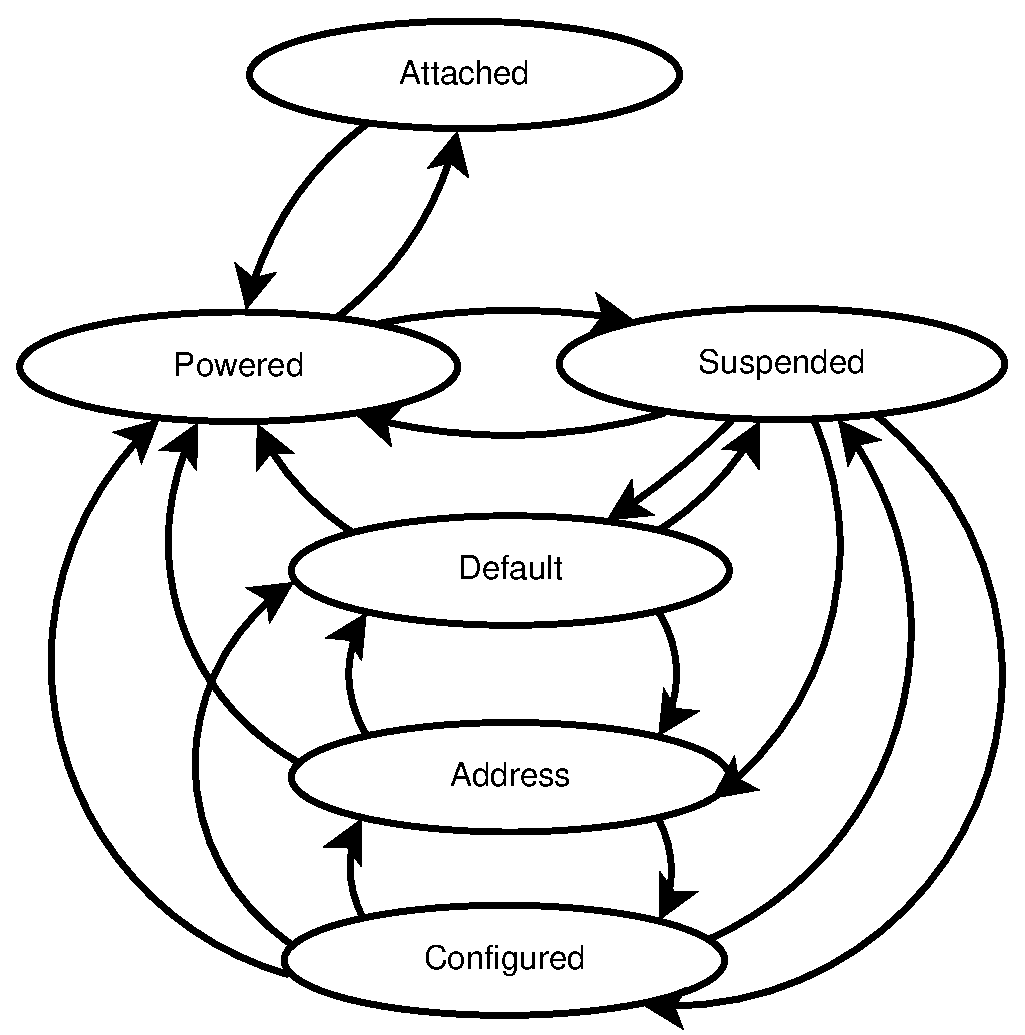
\includegraphics[width=8cm]{images/devzustand}
\caption{Ger�tezustandsdiagramm}
\label{devzustand}
}
\end{figure}
\index{Enmumerierung}

\textbf{1. USB-Ger�t wird angesteckt (Attached):}
Das USB-Ger�t wird angesteckt oder der Strom wird beim Systemstart eingeschaltet.
\newline\newline
\textbf{2. Ger�t wird erkannt (Powered, Suspended):}
Der Root-Hub oder ein anderer Hub meldet dem Host das neu gefundene Ger�t.
\newline\newline
\textbf{3. Reset des Ger�ts wird vorgenommen (Default):}
Der Host veranlasst entweder �ber den Root-Hub oder den Hub einen Reset des neuen Ger�ts. Durch
diesen Reset wird das Ger�t gezwungen, die Adresse 0 anzunehmen. Dadurch
kann der Host nach dem Reset das Ger�t �ber die Adresse 0 ansprechen.
\newline\newline
\textbf{4. Ermitteln der maximalen Paketgr��e f�r die Standard-Pipe (Default):}
Um die Gr��e des Endpunkt 0 herauszubekommen, sendet der Host eine \glqq{}GetDescriptor\grqq{}-Anfrage
f�r den Ger�te-Deskriptor an das Ger�t. Das USB-Ger�t antwortet mit den ersten acht Byte 
des Ger�te-Deskriptors. Da das achte Byte die Gr��e des Endpunkt 0 FIFOs enth�lt, stoppt
der Host die Antwort des USB-Ger�tes.
\newline\newline
\textbf{5. Ger�t bekommt eine Adresse zugewiesen (Address):}
Da der USB-Host nun die genaue Paketgr��e f�r den Enpunkt 0 kennt, kann
er die Pakete in der richtigen Gr��e an das USB-Ger�t schicken. Die erste
Anfrage ist \glqq{}SetAddress\grqq{}, mit der dem Ger�t eine endg�ltige Adresse zugewiesen wird.
\newline\newline
\textbf{6. Informationen vom Ger�t werden abgefragt (Address):}
Anschlie�end fragt der Host �ber die neue Adresse alle Ger�teinformationen ab.
\newline\newline
%\item[Treiber werden geladen:]
%Anhand der Ger�teinformationen kann das Betriebssystem einen geeigneten Treiber laden.
\textbf{7. Konfiguration wird gew�hlt (Configured):}
Um mit dem Ger�t Daten austauschen zu k�nnen, muss eine Konfiguration aktiviert werden.
\newline\newline

Mit dem Beispiel aus Abbildung \ref{beispiel} soll verdeutlicht werden, wie die Deskriptoren zusammenh�ngen und angeordnet sein m�ssen.
\begin{figure}[h]
{
\centering
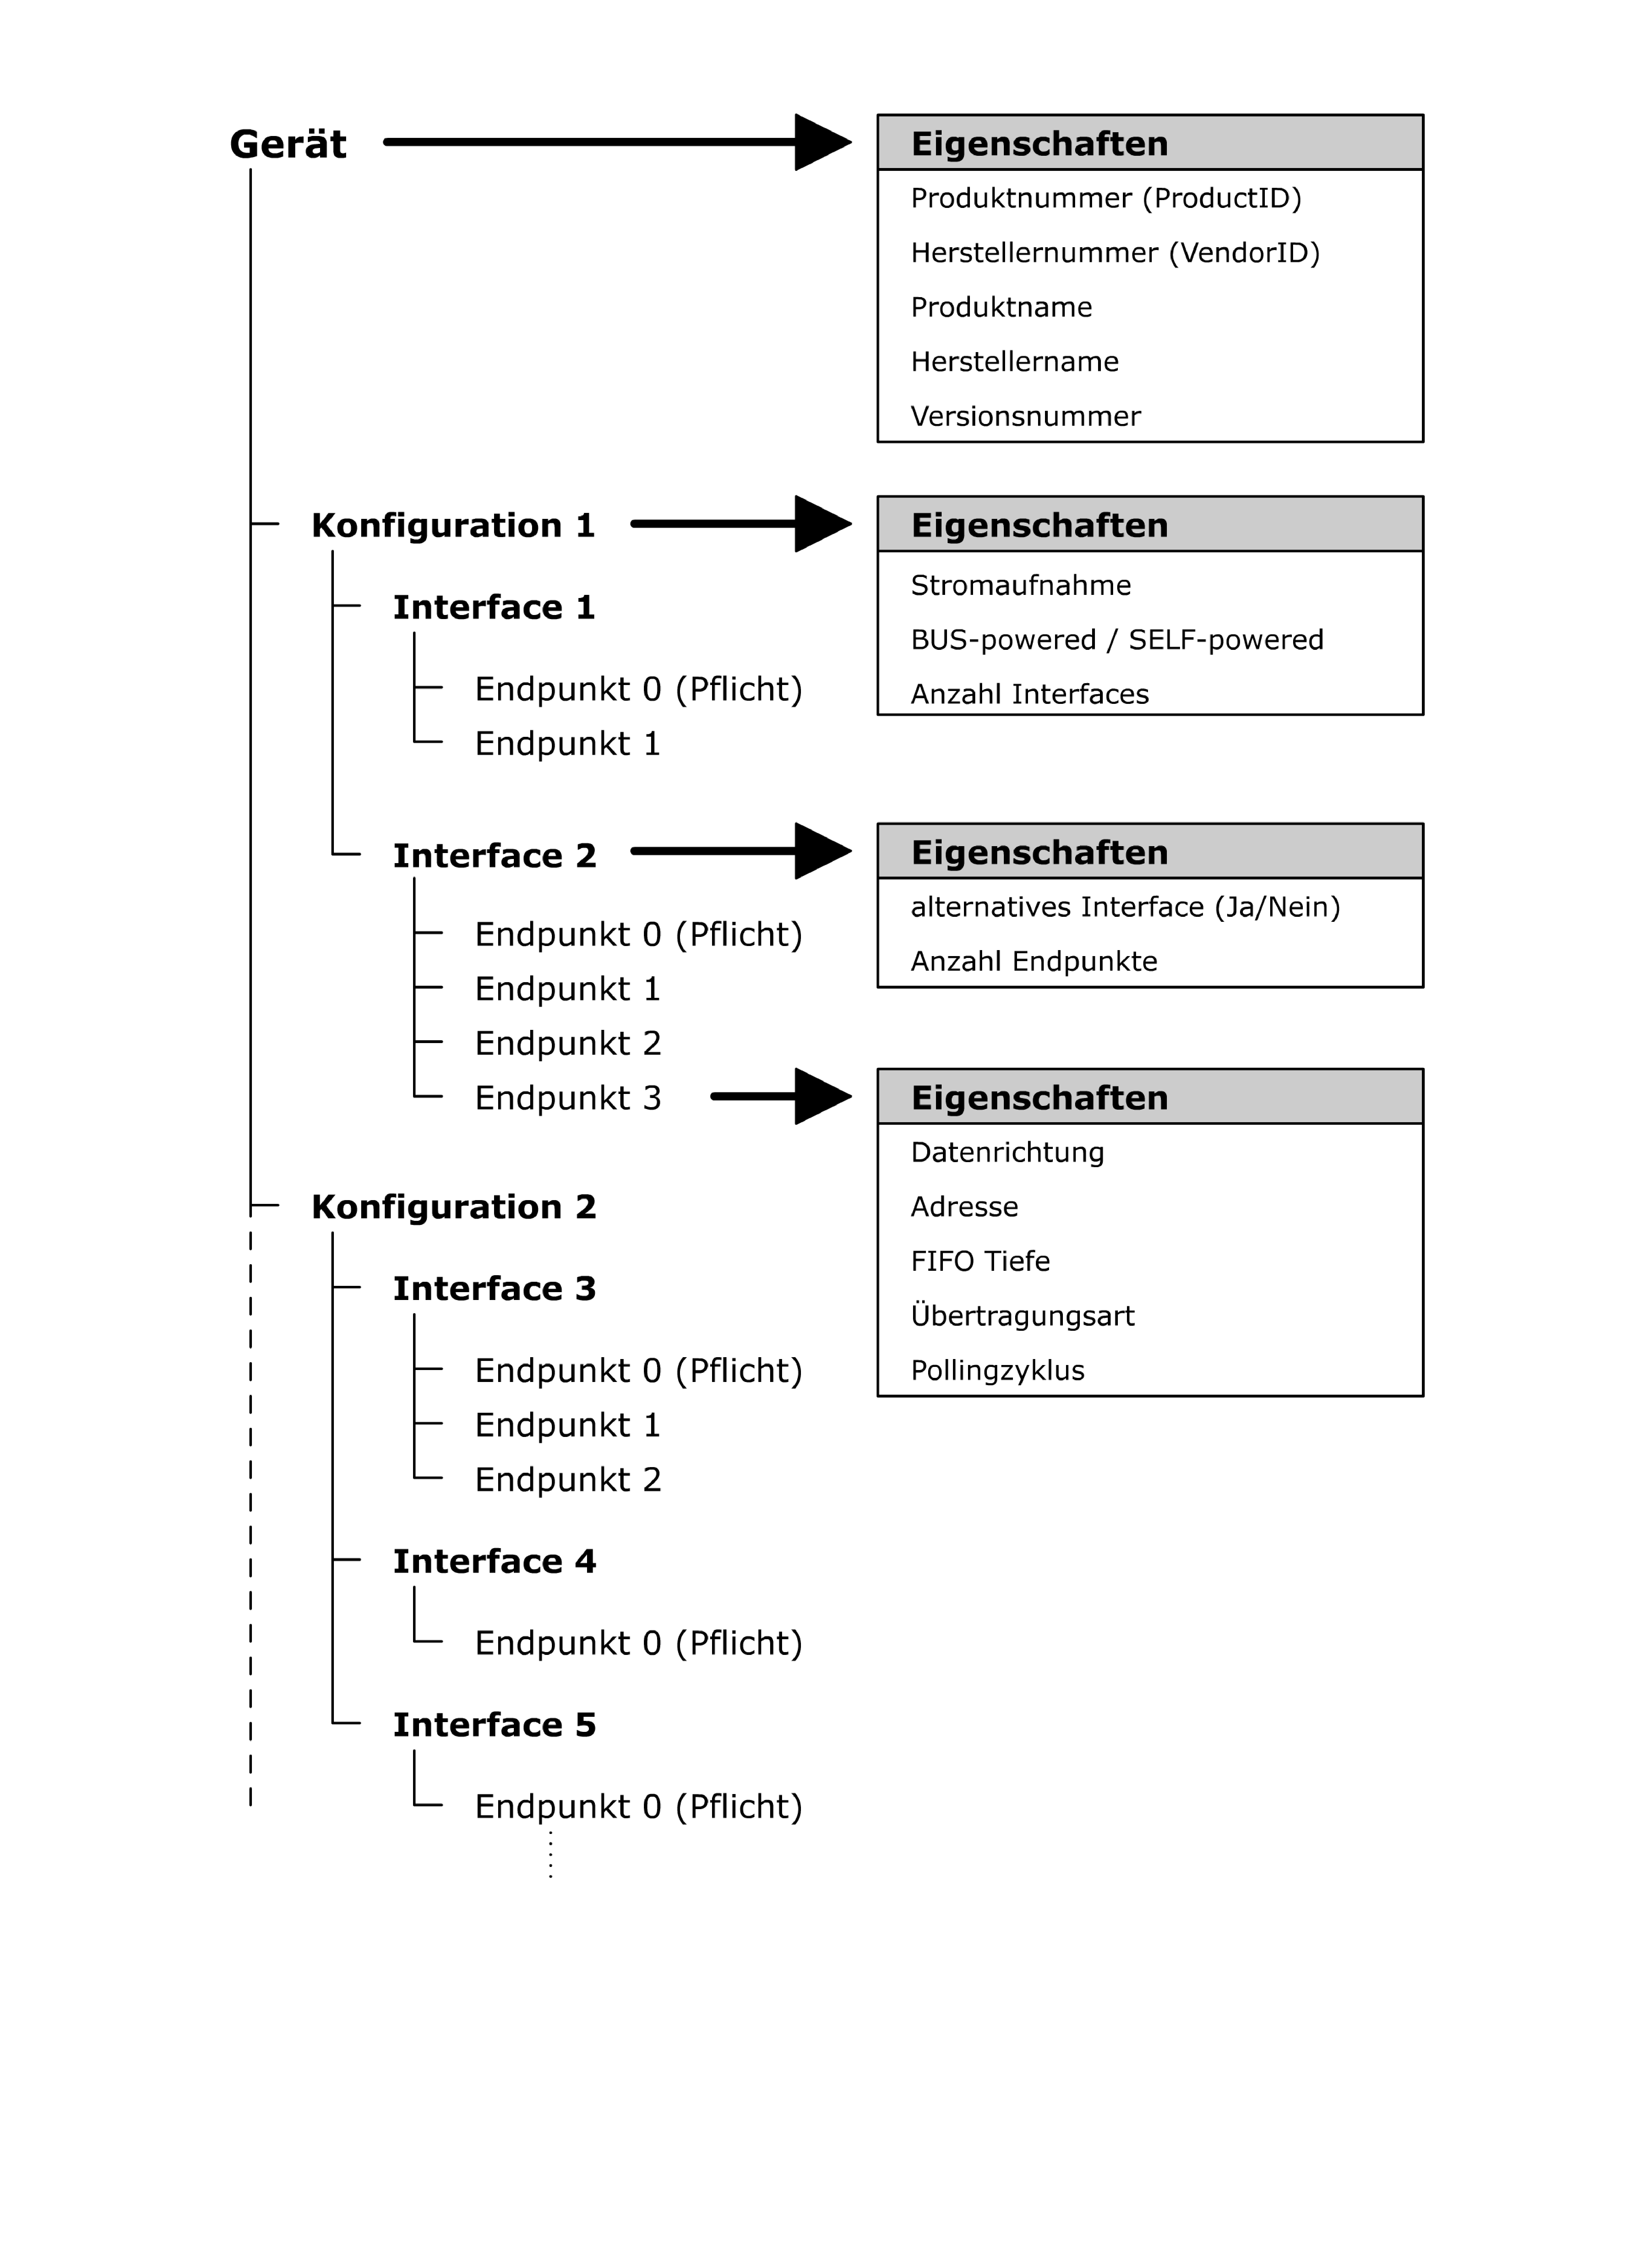
\includegraphics[width=15cm]{images/beispiel}
\caption{Beispiel-Deskriptoren}
\label{beispiel}
}
\end{figure}



	
\chapter{Die Komponenten und ihre Aufgaben im USB-Host-Stack}


Ein guter Entwurf der Struktur des USB-Stacks ist eine wichtige Basis f�r
die Stabilit�t und die Leistungsf�higkeit der gesamten Software. In diesem Kapitel werden die wichtigsten 
Komponenten des USB-Stacks und deren Aufgaben beschrieben.
Es wird ausschlie�lich auf die theoretischen Hintergr�nde
eingegangen und erst sp�ter im n�chsten Kapitel wird die Struktur und
die Umsetzung in Quelltext erkl�rt.

\section{Host-Stack}

Der USB-Stack wurde, soweit es m�glich und machbar war
nach der USB-Spezifikation implementiert. 
Da die USB-Spezifikation f�r einen Softwarestack auf einem 
PC geschrieben wurde, musste bei der Realisierung des Host-Stack f�r 
ein Embedded System Nutzen und Aufwand in Einklang gebracht werden.

\subsection{�bersicht des Protokoll-Stacks}

\index{Protokoll-Stack}

Der USB-Stack beinhaltet vom Hardwaretreiber bis hin zu den verschiedenen Ger�tetreibern alle Softwarekomponenten (siehe Abbildung \ref{struktur}), 
die f�r den USB-Betrieb n�tig sind.
F�r die
einzelnen Aufgaben wurden jeweils gesonderte Module entwickelt, welche ihre Dienste
�ber definierte Schnittstellen anbieten. 

\begin{figure}[h]
{
\centering
\includegraphics[width=11.5cm]{images/struktur}
\caption{Architektur des USB-Stacks}
\label{struktur}
}
\end{figure}

\index{Host-Controller}
\index{Host-Controller-Treiber}
\index{USB-Bustreiber}
\index{Host-Controller-Driver-Interface}
\index{USB-Bustreiber-Interface}

Auf diese Weise kann der Stack flexibel erweitert und in Anwendungen
integriert werden. Unterst�tzt der Stack eine bestimmte Aufgabe oder einen gewissen
Baustein nicht, so muss nur die fehlende Funktionalit�t nachprogrammiert und in 
das bestehende System eingebunden werden. 
\newline\newline
Im folgenden Abschnitt werden die wichtigen Bezeichnungen aus der Abbildung \ref{struktur} 
zur besseren �bersicht durch Fettdruck hervorgehoben.
\newline\newline
Der Softwarestack bietet f�r die Daten�bertragung verschiedene Ebenen an, die die Nachrichten �ber
USB durchlaufen m�ssen. Die unterste Ebene beinhaltet die physikalische Verbindung auf den USB-Bus.
Realisiert wird diese mittels des \textbf{Host-Controllers (Hardware)}. F�r den Host-Controller
wird ein Treiber ben�tigt, der die Kommunikation mit dem Baustein erm�glicht. Dies ist bereits die Aufgabe
der zweiten Ebene des \textbf{Host-Controller-Treibers (HCD)}.
Die notwendige Verbindung vom Host-Controller-Treiber zum \textbf{USB-Bustreiber (USBD)}, der eine Ebene
�ber dem HCD liegt, wird \textbf{Host-Controller-Driver-Interface (HCDI)} genannt.
Das HCDI bietet f�r den USB-Bustreiber allgemeine Funktionen f�r die Kommunikation mit einem beliebigen Host-Controller an.
Soll ein neuer Host-Controller in den Stack integriert werden, 
so m�ssen nur die Funktionen des HCDI f�r den neuen Controller programmiert werden.
\newline\newline
Auf der dritten Ebene befindet sich der USB-Bustreiber. Er bildet die zentrale Verwaltungs- und
Steuerungskomponente. In dieser Ebene werden Ger�te bzw. Treiber verwaltet und Datenstr�me verteilt.
Der USB-Bustreiber bietet seine Funktionen (Datenkommunikation, Ger�te- und Treiberverwaltung) 
�ber das \textbf{USB-Bustreiber-Interface (USBDI)}
den dar�ber liegenden Schichten an. Die Ger�te bzw. die Treiber aus den dar�ber liegenden Schichten k�nnen nie direkt mit
dem Host-Controller kommunizieren, sondern m�ssen immer �ber das USBDI gehen.
\newline\newline
Zu guter Letzt k�nnen die \textbf{Anwendungen} die Dienste �ber die entsprechenden
Treiberschnittstellen der \textbf{Ger�te- und Klassentreiber} nutzen.

\subsection{Datenfluss einer USB-Nachricht}
\index{USB-Nachricht}
\index{USB-Pakete}
\index{Transfer-Deskriptoren}
\index{I/O-Request-Paket}

In diesem Abschnitt wird der Verlauf einer USB-Nachricht
im USB-Stack betrachtet. 
\newline\newline
Eine USB-Nachricht ist eine Anfrage einer Anwendung bzw. eines Treibers, die �ber
das USBDI \footnote{\label{foot:usbdi} \glqq{}USB-Bustreiber-Interface\grqq{} enth�lt alle Funktionen f�r den Datenaustausch mit Ger�ten.} 
abgesendet werden kann. Eine USB-Nachricht enth�lt entweder Daten f�r
das Ger�t, oder eine Anfrage f�r Daten vom Ger�t. 
Die Nachricht muss immer mit der entsprechenden Transferfunktion aus dem USBDI mit
der Transferart des Zielendpunktes �bertragen werden.
\newline\newline
Eine USB-Nachricht sieht, unabh�ngig von der Transferart, strukturell
immer gleich aus. Es muss die Ger�teadresse, der Endpunkt, die Transferart, die �bertragungsrichtung,
eine Anzahl und ein Puffer f�r die zu sendenden oder zu empfangenden Daten angegeben werden.
In der USB-Spezifikation wird diese Datenstruktur \glqq{}I/O-Request-Packet (IRP)\grqq{} genannt.
M�chte eine Anwendung oder ein Treiber Daten versenden, so muss solch eine Anfrage erzeugt
und dem USB-Bustreiber �bergeben werden. 
\newline\newline
Wie bereits erw�hnt, werden auf dem USB-Bus aber nur USB-Pakete �bertragen. Dies bedeutet
f�r den Host, dass er die vorliegende USB-Nachricht in einzelne Pakete aufteilen muss (siehe Abbildung \ref{irp}).
Abh�ngig von der Transferart werden SETUP-, IN-, OUT-, DATA0- oder DATA1-Pakete generiert. Diese einzelnen
Pakete werden in einer Datenstruktur, die Transfer-Deskriptor genannt wird, gepackt. Ein Transfer-Deskriptor
enth�lt die kleinste USB-Einheit, die mit einem Host-Controller �bertragen werden kann - ein USB-Paket.
\newline\newline

\begin{figure}[h]
{
\centering
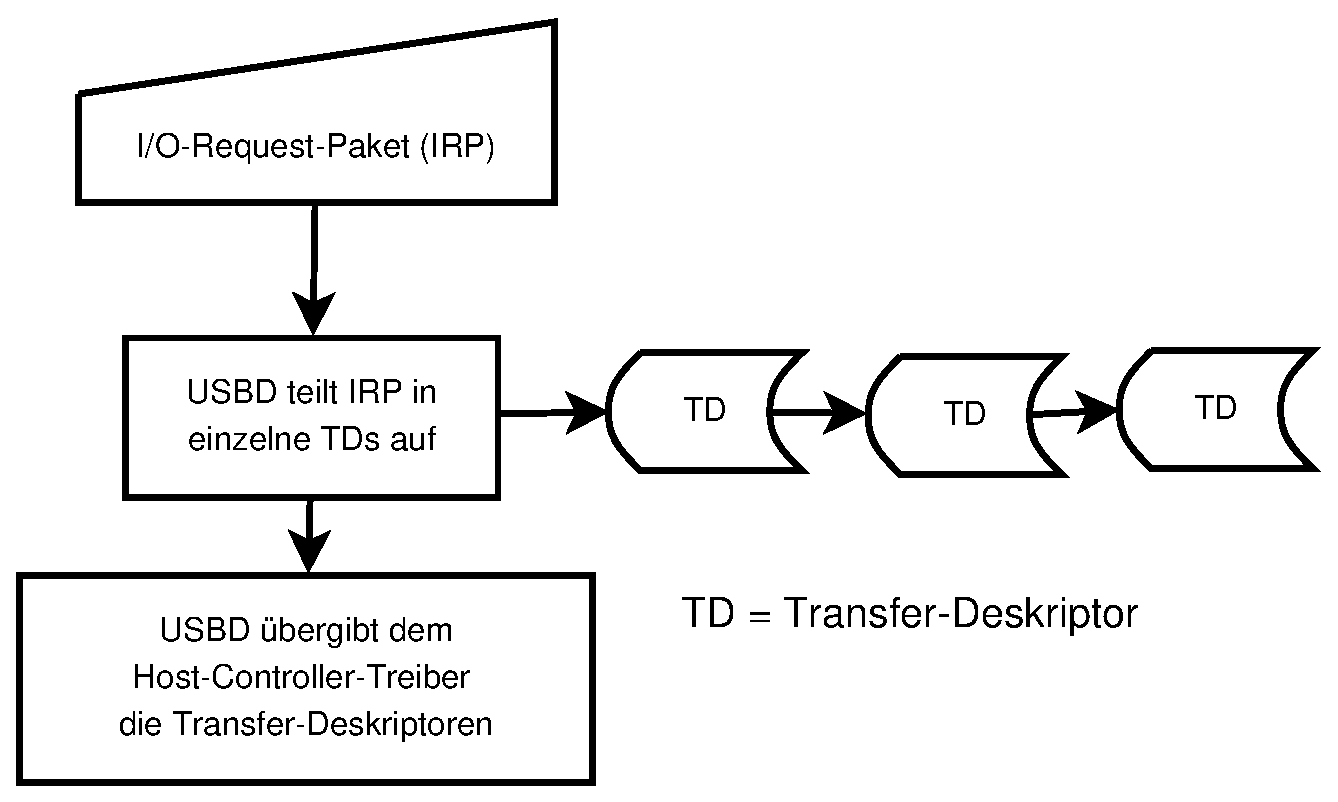
\includegraphics[width=11.5cm]{images/irp}
\caption{Aufteilung der I/O-Request-Pakete in Transfer-Deskriptoren}
\label{irp}
}
\end{figure}
Die Aufteilung ist unter anderem daf�r notwendig, dass die am Bus angeschlossenen
Ger�te mit gleicher Priorit�t behandelt werden k�nnen.
Mehr dazu im n�chsten Absatz \glqq{}Verteilung der Bandbreite\grqq{}.

\subsection{Verteilung der Bandbreite}
\index{Bandbreite}
W�rde ein Treiber zum Beispiel 1 MB Daten an ein Ger�t senden, w�re der
Bus theoretisch bei 12 MBit/s f�r 1,5 s belegt. Betreibt man parallel am Bus
zus�tzlich eine USB-Maus, so k�nnte in dieser Zeit die Maus nicht erreicht und somit
der Mauszeiger nicht aktualisiert werden.
Daher ist es notwendig, dass USB-Nachrichten
durch Segmentierung in einzelne USB-Pakete (\glqq{}Transfer-Deskriptoren\grqq{}) aufgeteilt werden
und einzeln nach und nach abwechselnd mit Paketen von anderen Nachrichten versendet werden. 
Dadurch kann der Host in einer Zeitspanne,
die durch Frames aufgeteilt ist (siehe Kapitel 3.8), mehrere Ger�te ansprechen.
\newline\newline
Mit welcher Strategie die zur Verf�gung stehende Zeit verteilt werden muss, ist in der USB-Spezifikation nicht beschrieben.
Die USB Spezifikation gibt nur an, wieviel Zeit f�r welche Transferart reserviert sein muss (siehe Tabelle \ref{usb_zeiten}).

\begin{table}[h]
\center
\begin{tabular}{|l|l|}
\hline
\rowcolor{Gray}[0.9\tabcolsep]
Transferart & Bandbreite \\ \hline
Control & max. 10\% garantiert \\ \hline
Interrupt und Isochron & max. 90\% garantiert \\ \hline
Bulk & nur bei verf�gbarer Bandbreite \\ \hline
\end{tabular} \caption{Garantierte Bandbreiten der Transferarten} \label{usb_zeiten}
\end{table}

\subsection{Status�berwachung}
\index{Status�berwachung}
Da der USB-Bustreiber alle wichtigen Komponenten verbindet, bietet er sich ideal
f�r die �berwachung des Busses an. Die Auslastung auf dem Bus kann z.B. anhand 
der Anzahl der �bertragenen Pakete ermittelt werden oder auch die korrekte Arbeitsweise der
USB-Ger�te und des Host-Controllers mit speziellen Funktionen der Treiber.
In der USB-Spezifikation ist nicht definiert, welche Informationen �berwacht werden sollen,
es wird nur angeregt, dies an der gerade genannten Stelle im USB-Bustreiber zu integrieren.
\newpage

%Sogenannte USB Debug Monitor, die den Datentransfer f�r eine Analyse
%des Datenstroms aufzeichnen bieten sich ebenfalls an dieser Stelle zu integrieren.

\section{Host-Controller}
\index{Host-Controller}
Der Host-Controller ist verantwortlich f�r die Generierung 
der �bertragungen der einzelnen USB-Pakete, eingepackt in die
Transfer-Deskriptoren.

\subsection{Aufbau und Struktur}

In allen Implementierungen f�hren Host-Controller die gleichen grundlegenden Aufgaben 
hinsichtlich des USB-Busses und seiner verbundenen Ger�te durch. In der USB-Spezifikation
werden die einzelnen Teilkomponenten (Abbildung \ref{host}), die daf�r notwendig
sind, beschrieben.

\begin{figure}[h]
{
\centering
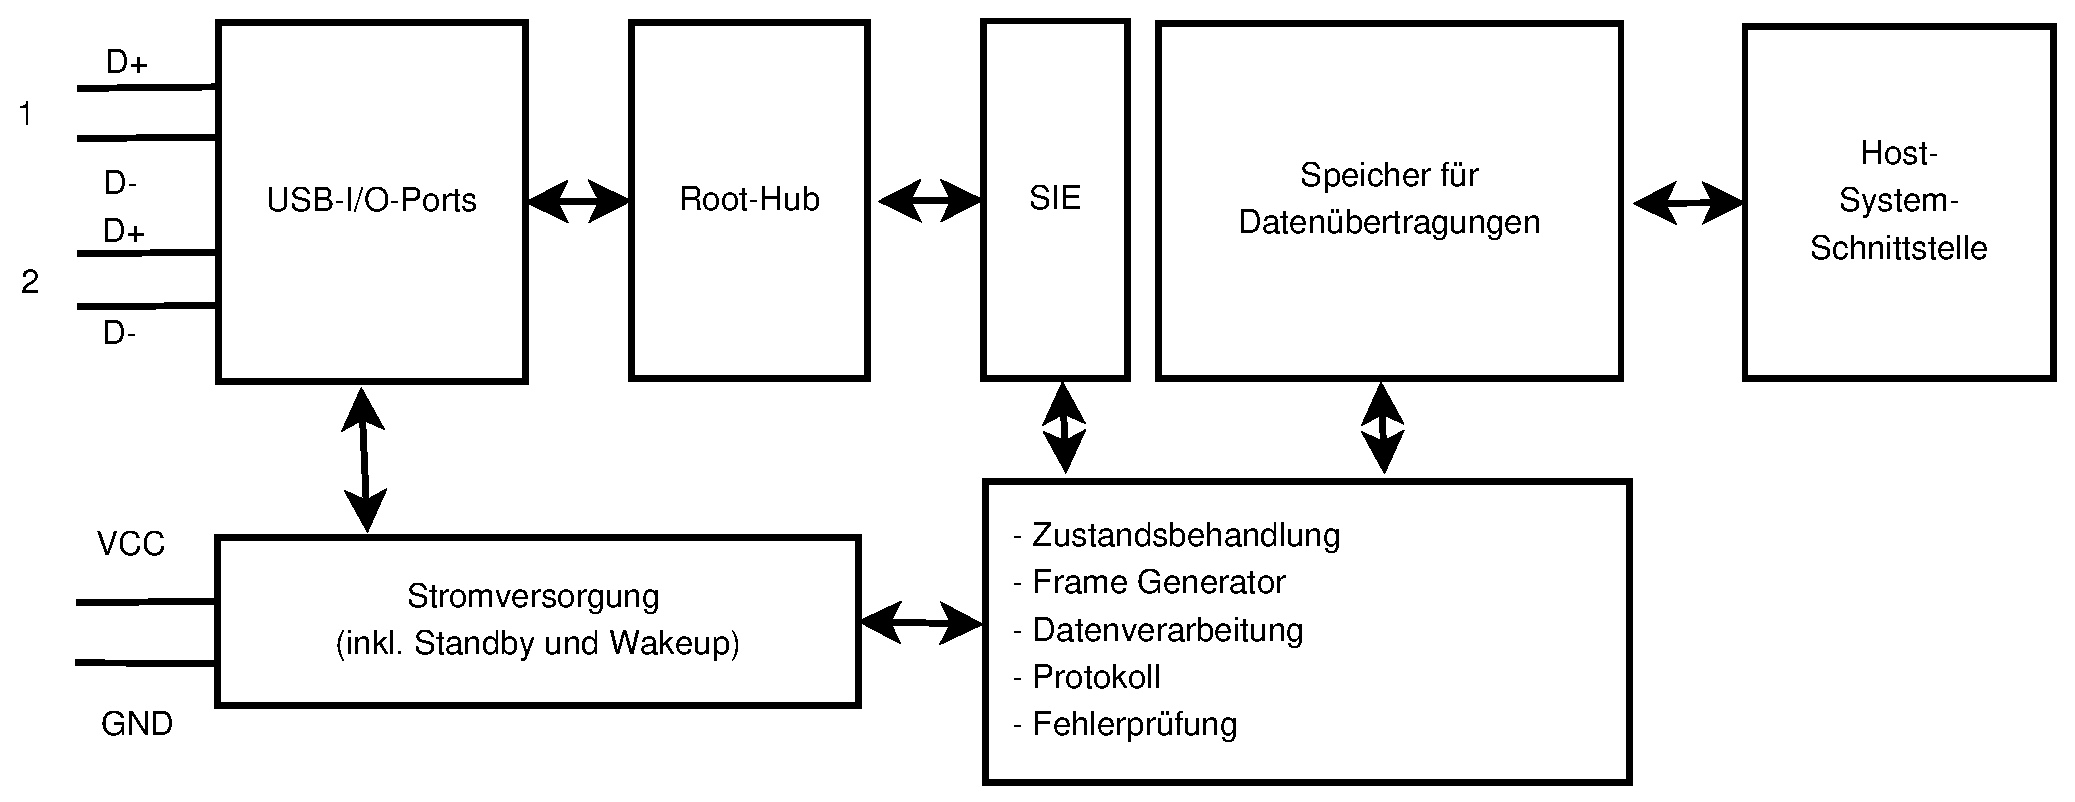
\includegraphics[width=15cm]{images/host}
\caption{Host-Controller Strukturdiagramm}
\label{host}
}
\end{figure}


\index{SIE}
\index{Root-Hub}

\begin{description}
\item[Zustandsbehandlung:] 
Der Host-Controller kann viele Ereignisse und Zust�nde vom USB-Bus
�ber interne Register und Signale anzeigen. Diese Zust�nde
werden vom USB-Stack f�r den Betrieb des USB-Busses ben�tigt.

\item[Serialisierer und Deserialisierer (\glqq{}SIE\grqq{}):] 
Um die Daten �bertragen und empfangen zu k�nnen, muss der Host-Controller,
wie in Kapitel \ref{kap:signal} auf Seite \pageref{kap:signal} beschrieben, die Daten zum Senden serialisieren und codieren
und beim Empfangen wieder decodieren und parallelisieren.


\item[Rahmenerzeugung (\glqq{}Frame Generation\grqq{}):] 
Der Host-Controller ist zust�ndig f�r die Einteilung des Busses in die einzelnen Frames.
Daf�r muss jede Millisekunde ein Start-of-Frame Paket (SOF) mit einer fortlaufenden
Nummer versendet werden.
�ber interne Zeitgeber kann der Host-Controller dies automatisch erledigen.


\item[Datenverarbeitung:] 
Der Host-Controller ist f�r das Empfangen
und das Senden von Daten (USB-Paketen) verantwortlich. 

\item[Protokoll:]
Die passenden Protokollinformationen f�r ausgehende Anfragen m�ssen zusammengesetzt werden und
eingehende Anfragen zerlegt und interpretiert werden.

\item[Fehlerbehandlung bei der �bertragung]
Der Host-Controller muss Datentransportfehler erkennen k�nnen. In
der USB-Spezifikation sind die folgenden Fehlerarten beschrieben:

\begin{itemize}
\item \glqq{}Timeout-Fehler\grqq{} nach Datentransfer. Diese treten auf, wenn die
Endpunktadresse nicht existiert, oder die zu �bertragenden Daten so
fehlerhaft sind, dass diese vom USB-Ger�t nicht interpretiert werden k�nnen.
\item Fehlende oder fehlerhafte Daten:

\begin{itemize}
\item Der Host-Controller sendet oder empf�ngt ein zu kurzes Paket.
\item Ein empfangenes Paket enth�lt eine ung�ltige CRC Pr�fsumme.
\end{itemize}

\item Protokollfehler:
\begin{itemize}
\item Ein ung�ltiges \glqq{}Handshake-Packet\grqq{}.
\item Ein falsches \glqq{}End-of-Packet (EOP)\grqq{}.
\item Ein Bitstuffing-Fehler.
\end{itemize}
\end{itemize}

\item[Entferntes Aufwecken (\glqq{}Wakeup\grqq{}):] 
Das USB-System kann den Bus jederzeit in den Zustand Standby versetzen
und anschlie�end wieder aufwecken.
Daf�r muss der Host-Controller entsprechende Vorrichtungen anbieten.

\item[Root-Hub:] 
Der Root-Hub stellt die Verbindung zwischen dem Host-Controller
und den Anschlussports f�r Ger�te her. Die Arbeitsweise
ist gleich dem Hub (siehe Seite \pageref{kap:hub}). Der einzige Unterschied
besteht in der Anbindung an das System. So ist ein Root-Hub
im Gegensatz zum Hub, der �ber USB angesprochen wird
�ber interne Signale mit dem Host-Controller verbunden.

\item[Host-System-Schnittstelle:] 
Die Schnittstelle f�r den Datenaustausch zwischen dem Host-Controller
und dem Prozessor, auf dem der USB-Stack l�uft.
\end{description}

\subsection{Daten�bertragung mit Host-Controllern} \label{kap:datenuebertragung}
\index{Daten�bertragung}
\index{OHCI}
\index{EHCI}
\index{UHCI}
\index{USB-Nachricht}
\index{Transfer-Deskriptor}
\index{I/O-Request-Paket}
Im vorherigen Abschnitt wurden alle Funktionen,
die ein Host-Controller anbieten muss, kurz beschrieben. F�r die Implementierung
des USB-Stacks in dieser Diplomarbeit soll die Funktionsweise der
Daten�bertragung, speziell f�r Host-Controller in Embedded Systeme, genauer betrachtet werden.
\newline\newline
Wie die �bertragung auf dem Host-Controller genau
funktioniert, ist in dem Hauptdokument der USB-Spezifikation nicht beschrieben.
Dies war die Aufgabe der Host-Controller Hersteller. F�r USB 1.1 wurden
zwei Standards entwickelt, das UHCI (\glqq{}Universal-Host-Controller-Interface\grqq{})  und das
OHCI (\glqq{}Open-Host-Controller-Interface\grqq{}). UHCI kompatible Bausteine
kommen mit weniger Transistoren aus, da dort ein Gro�teil
der Steuerung mit Software erledigt wird. OHCI im Gegenzug verlagert
viele der Verwaltungsaufgaben in die Hardware und bietet daher eine einfachere
Schnittstelle an. UHCI wurde von Intel, und  OHCI
gemeinsam von Compaq, Microsoft und National Semiconductor entwickelt.
F�r USB 2.0 wurde von allen beteiligten Firmen ein gemeinsamer Standard EHCI (Enhanced-Host-Controller-Interface) definiert.
\newline\newline
Obwohl sich alle drei Standards doch sehr unterscheiden, gibt es trotzdem eine gemeinsame Eigenschaft - bedingt dadurch, dass
alle Controller f�r den Einsatz im Computer entwickelt worden sind -
n�mlich die �bergabe der kompletten Transfer-Deskriptoren �ber einen gemeinsamen Arbeitsspeicherbereich
zwischen dem Prozessor und dem Host-Controller. 
\newline\newline
Sendet ein Treiber oder eine Anwendung eine USB-Nachricht ab, so wird direkt ein Speicherbereich
aus dem gemeinsamen Arbeitsspeicher zwischen Prozessor und Host-Controller f�r die Kommunikation genutzt (siehe Abbildung \ref{cpu2host}). Die Software
muss lediglich die Datenstruktur richtig aufbauen, so dass die Hardware die 
einzelnen Transfer-Deskriptoren erreichen kann. Wird der letzte Transfer-Deskriptor
eines I/O-Request-Paketes erfolgreich abgearbeitet, so muss
dies die Hardware nur noch der Software signalisieren, welche dann wiederum dem
Treiber oder der Anwendung meldet, dass die Daten in dem zuvor reservierten
Speicher eingetroffen sind.

\begin{figure}[h]
{
\centering
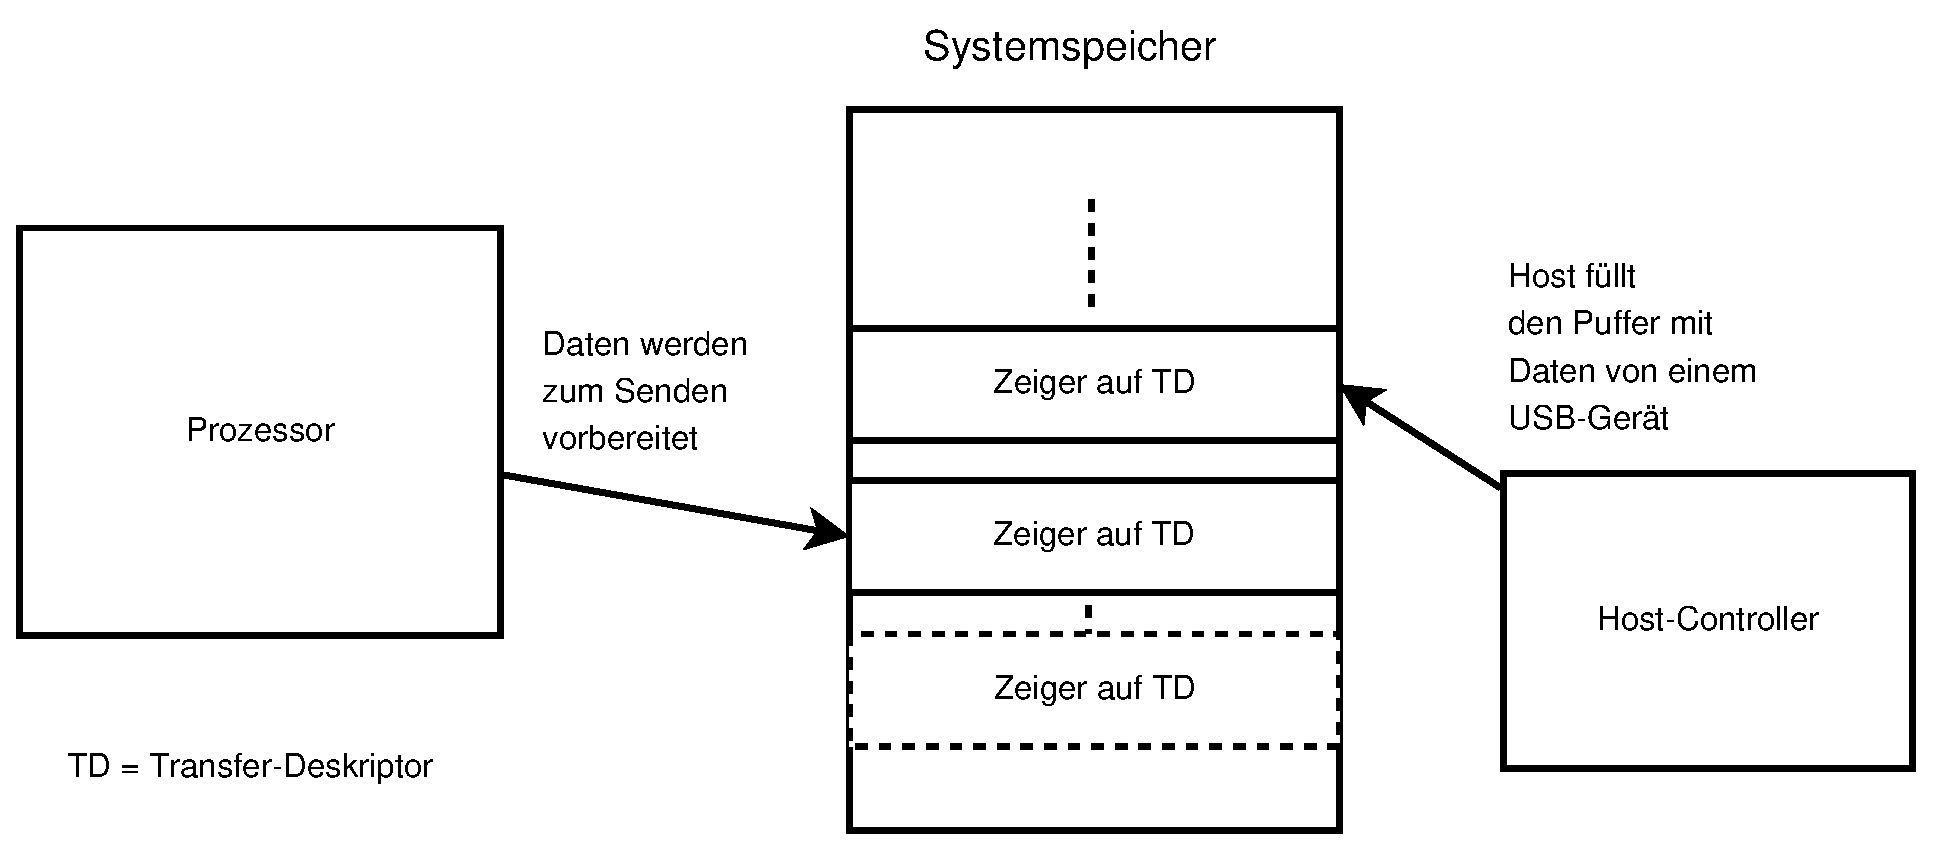
\includegraphics[width=15cm]{images/cpu2host}
\caption{Gemeinsamer Speicher von Prozessor und Host-Controller}
\label{cpu2host}
}
\end{figure}

Bei Mikroprozessoren hingegen muss die �bergabe aber oft �ber I/O-Zugriffe oder spezielle Schnittstellen realisiert
werden, da es dort h�ufig nicht m�glich ist, mit Peripherie Speicherbereiche zu teilen.
Das bedeutet, dass jede �bergebene Transaktion sofort ausgef�hrt werden muss und ein Ergebnis f�r
die weitere Verarbeitung des USB-Pakete-Datenstroms erforderlich ist.
\newline\newline
Damit alle Host-Controller-Typen im USB-Stack genutzt werden k�nnen,
�bergibt der USB-Bustreiber dem Host-Controller-Treiber immer
einzelne Transfer-Deskriptoren. In den Transfer-Deskriptoren
befindet sich aber wiederum ein Zeiger auf das dar�ber liegende
I/O-Request-Paket (siehe Abbildung \ref{td2irp}).
So kann in den Treibern abh�ngig vom Baustein
entschieden werden, wie die Abarbeitung stattfinden soll.

\begin{figure}[h]
{
\centering
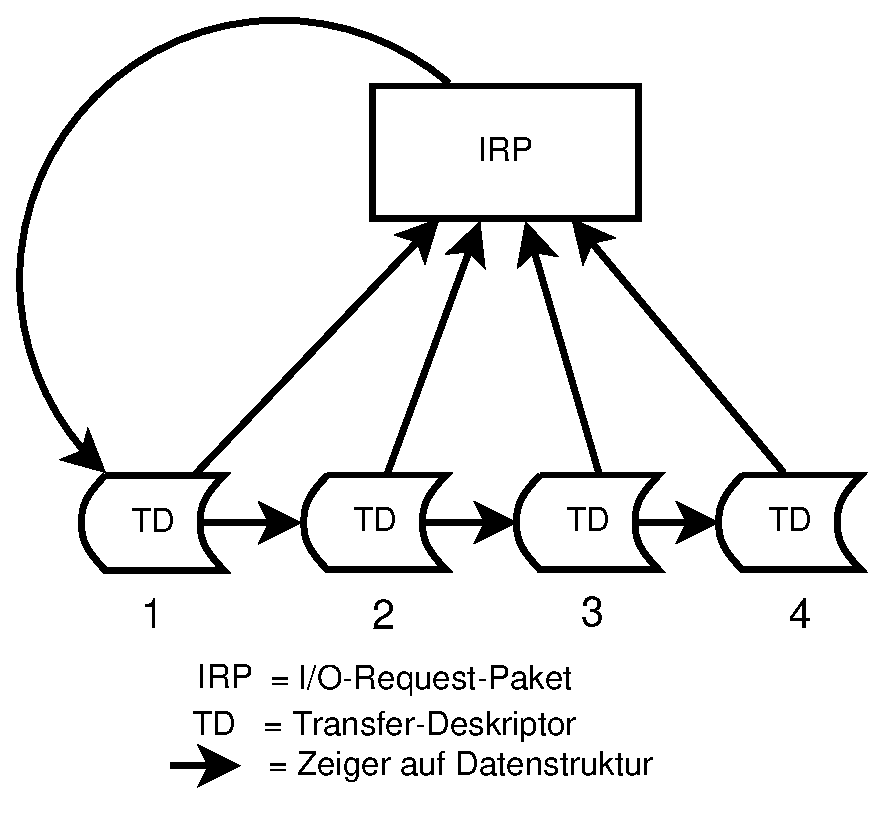
\includegraphics[width=8cm]{images/td2irp}
\caption{Verkettung der Datenstrukturen IRP und TD}
\label{td2irp}
}
\end{figure}

%\subsection{OHCI kompatibler Controller}
%Das OHCI (Open-Host-Controller-Interface) stammt von Compaq, Microsoft
%und National Semiconductor. Implementiert ist OHCI typischerweise in dedizierten Chips�tzen.
%
%\subsubsection{�bertragungsreihenfolge}
%\begin{figure}[h]
%{
%\centering
%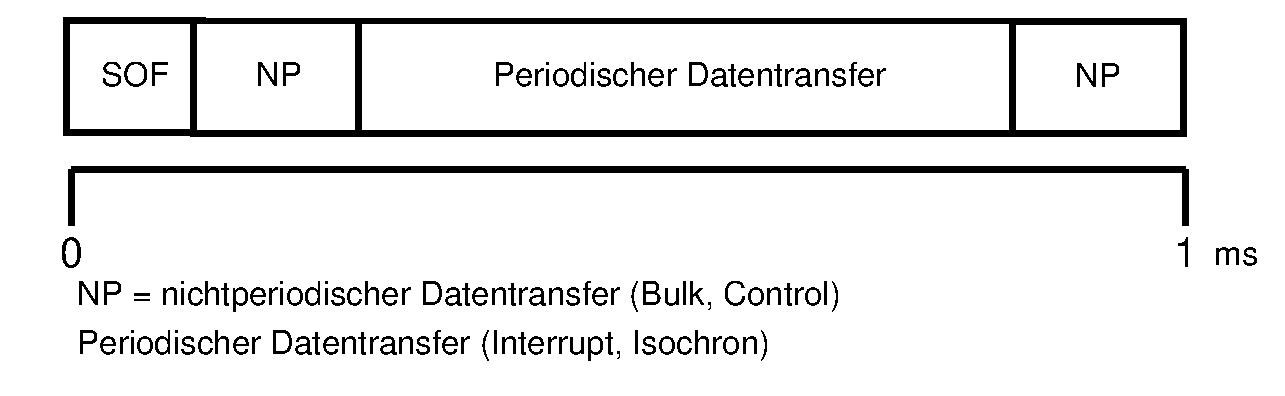
\includegraphics[width=14cm]{images/ohci_zeit}
%\caption{�bertragungsreihenfolge OHCI}
%\label{ohci_zeit}
%}
%\end{figure}
%\subsubsection{Transfermechanismus}
%\begin{figure}[h]
%{
%\centering
%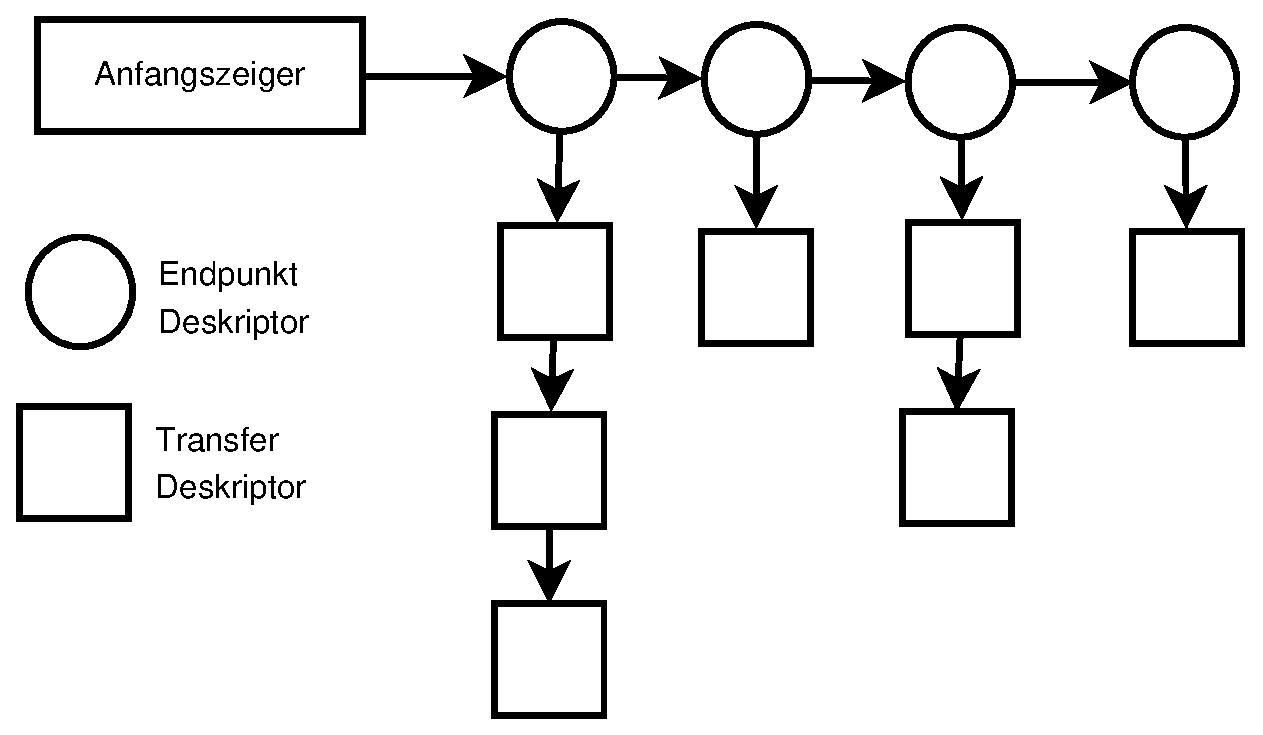
\includegraphics[width=11cm]{images/ohci}
%\caption{Transfermechanismus OHCI}
%\label{ohci}
%}
%\end{figure}
%\subsubsection{Enpunkt-Deskriptoren}
%\subsubsection{Transfer-Deskriptoren}
%\subsubsection{OHCI Register}
%\subsection{UHCI kompatibler Controller}
%Die UHCI (Universal-Host-Controler-Interface) Spezifikation wurde von Intel erstellt.
%Das Interface ist ebenfalls wie das OHCI meist in Chips�tzen integriert. Die Komplexit�t
%des UHCI wird von Intel mit etwa 10K Gates angegeben.
%\subsubsection{�bertragungsreihenfolge}
%\subsubsection{Frame-Listen}
%\subsubsection{Transfer-Mechanismus}
%\subsubsection{Transfer-Deskriptoren}
%\subsubsection{Queue-Heads}
%\subsubsection{UHCI Register}
%
%\subsection{EHCI kompatibler Controller}
%
%Mit der Spezifikation USB 2.0 wurde gleich ein Standard Host-Controller ver�ffentlicht,
%welcher die Erweiterungen zum High-Speed Modus beinhaltet und gleichzeitig Abw�rtskompabilit�t gew�hrleisten
%soll.
%
%
%\subsubsection{Architektur}
%\subsubsection{Host-Controller-Routing-Strategie}
%\subsubsection{Datenstrukturen}
%
%\subsection{Phillips kompatible Controller}
%
%Es gibt auch Controller die diesem Standard nicht entprechen. Vorallem im Embedded Bereich,
%denn hier hat man selten einen gemeinsamen speicherbereich. Meistens eine
%Port oder eine andere schnittstelle
%
%beispiel phillips mach beides mit den PTD

%\section{Integrierter Root-Hub-Controller}

%Die Aufgabe eines USB Hubs ist das Anzeigen des aktuellen Status der Ports
%und �nderungen an ihnen. Aufgrund dieser Informationen kann der Hub Treiber
%den Host �ber �nderungen informieren, und der Host kann entsprechend
%eine Enumeration oder mit dem Entfernen von Datenstrukturen f�r ein
%entferntes Ger�t beginnen. 
%\newline\newline
%Da ein Host-Controller f�r die Signalisierung von �nderungen an dem
%abgehenden USB-Ports meistens Interrupt Signale und interne Status Register hat,
%welche f�r die Aufgaben des Root-Hubs notwendig sind,
%simuliert man dort einen echten USB-Hub, so dass man die Host-Ports �ber
%den gleichen Hubtreiber wie die f�r ein USB-Hub ansteuern kann und sich doppelte Arbeit spart.

\newpage
\section{Bandbreitenabsch�tzung}
\index{Daten�bertragungsrate}
\index{Bulk-Transfer}
Bei der Konzeption von USB-Ger�ten ist die Frage der maximalen
Daten�bertragungsrate oft von Interesse. Daher wird in diesem Abschnitt
eine Beispielrechnung vorgef�hrt, um zu zeigen, auf welche
Faktoren und Parameter geachtet werden muss, um die Kapazit�ten
des USB-Busses vollst�ndig auszunutzen.
\newline\newline
In der USB-Spezifikation sind die drei Ger�teklassen
Low-Speed-Ger�te (bis 1,5 MBit/s), Full-Speed-Ger�te (bis 12 MBit/s)
und High-Speed-Ger�te (bis 480 MBits/s ab USB Version 2.0) definiert.
Diese Angabe bezieht sich aber auf die physikalische maximale �bertragungsrate.
Soll die tats�chliche Datenrate ermittelt werden, m�ssen einige Parameter beachtet werden.
Im folgenden Beispiel wird eine Rechnung f�r einen Bulk-Transfer mit einem Full-Speed-Ger�t (12 MBit/s)
durchgef�hrt.
\newline\newline
In Kapitel \ref{pakzei} (Seite \pageref{pakzei}) wurde bereits beschrieben, dass Daten nach dem Start-of-Frame-Paket (SOF) versendet werden. 
Da das SOF-Paket jede Millisekunde vom Host generiert wird, bedeutet dies bei Full-Speed-Ger�ten (12 MBit/s),
dass maximal 12000 Bit (je Bit 83,33 ns) pro Millisekunde �bertragen werden k�nnen.
Die Gr��e der Daten-Pakete ist wiederum abh�ngig von der maximalen Endpunkt-Tiefe (siehe Taballe \ref{usb_bandbreite_full} und \ref{usb_bandbreite_high}), welche 
durch die Transferart bestimmt wird. Bei dem gew�hlten Bulk-Transfer mit Full-Speed-Ger�ten
kann ein Endpunkt-FIFO maximal 64 Byte (= 512 Bit) gro� sein. 
Ein weiterer Faktor f�r die Ermittlung der maximalen Daten�bertragungsrate ist der Overhead (Protokoll-Overhead und Bit-Stuffing),
der f�r ein Daten-Paket ben�tigt wird. F�r einen Bulk-Endpunkt ist dieser 13 Byte (= 104 Bit) gro�.
\newline\newline
Der entscheidendste Faktor ist aber der, wie oft ein Daten-Paket w�hrend einer Millisekunde an einen Endpunkt
gesendet werden kann.
Aus den Tabellen \ref{usb_bandbreite_full} und \ref{usb_bandbreite_high} kann entnommen werden, dass ein Bulk-Endpunkt bis zu 19 mal pro Frame angesprochen werden kann.
Wie dieser Wert zustande kommt, wird mit der nachstehenden Rechnung gezeigt:

\begin{eqnarray}
\text{max. �bertragungen} & = & \frac{\text{max. Anzahl Bits pro ms}}{\text{Overhead + max. FIFO-Tiefe}} \\[5mm]
\text{max. �bertragungen} & = & \frac{12000\text{ Bit}}{104\text{ Bit} + 512\text{ Bit}} \\[5mm]
& = & 19,48 \text{ �bertragungen pro Millisekunde}
\label{max_datenrate}
\end{eqnarray}

Mit der maximalen Anzahl an �bertragungen pro Frame kann im n�chsten Schritt die Berechnung der maximalen �bertragungsrate
durchgef�hrt werden.

\begin{eqnarray}
\text{max. �bertragungsrate} & = & \text{max. �bertragungen} * \text{max. FIFO-Tiefe}\\[5mm]
\text{max. �bertragungsrate} & = & 19 \text{ pro ms} * 512\text{ Bit} \\[5mm]
& = & 9,728\text{ MBit/s}
\end{eqnarray}

Mit 19 Paketen kann man also eine �bertragungsrate von ca. 9,7 MBit/s erreichen.
Die angenommenen 19 Pakete sind die theoretisch maximal M�glichen.
Ob alle Pakete innerhalb eines Frames auch versendet werden k�nnen,
h�ngt von dem eingesetzten Host-Controller ab. Wie bereits erw�hnt,
werden die Daten immer nach den SOF-Paketen, welche meist von den Host-Controllern
automatisch generiert werden, versendet.
Oft kann man sich das Absenden durch einen Interrupt signalisieren lassen.
Liegen  die Daten zu dem Zeitpunkt des Signalisierens bereits im Speicher, den der Host zum Versenden benutzt,
werden die ersten 64 Byte Daten plus Overhead f�r das erste Paket sofort versendet.
\newline\newline
Der weitere Verlauf ist abh�ngig von der Art des Host-Controllers.
Wie in Kapitel \ref{kap:datenuebertragung} auf Seite \pageref{kap:datenuebertragung} beschrieben, gibt es prinzipiell zwei Arten.
Die einen, bei den Pakete direkt aus einem gemeinsamen Speicher mit dem Prozessor �bertragen werden k�nnen,
und die anderen, bei denen jedes Paket �ber eine I/O-Schnittstelle �bergeben werden muss. 
F�r die Ermittlung der Datenrate werden beide F�lle f�r den weiteren Verlauf beschrieben.
\newline\newline
\textbf{1. Fall: Host nutzt gemeinsamen Speicher mit dem Prozessor: }
Wenn alle Pakete im Speicher bereit liegen, kann der Host-Controller nacheinander alle
Daten versenden.
\newline\newline
\textbf{2. Fall: Dem Host werden die Pakete �ber eine I/O-Schnittstelle �bergeben: }
Viele Host-Controller dieser Art bieten zwei Speicherbereiche f�r die Daten�bertragung an.
Dadurch kann, w�hrend der Inhalt des einen Speichers �bertragen wird, der zweite mit Daten gef�llt werden.
Dies wechselt sich immer ab, bis der Transfer beendet ist. F�r die I/O-Schnittstelle bedeutet dies aber, dass innerhalb
von min. 43 $\mu$s (512*83,33 ns) 64 Byte �bertragen werden m�ssen, damit die Daten rechtzeitig
in dem zweiten Speicher bereitstehen. Bei einem 8-Bit breiten I/O-Bus ben�tigt man
so, wenn man f�r den Verwaltungs-Overhead den Faktor 3 annimmt (Lese-, Schreib- und Adresssignale setzen), 
eine I/O-Geschwindigkeit von mindestens 5 MHz. 
\newline\newline
Angenommen, der Host-Controller hat nur einen Speicherbereich zum �bertragen der Daten,
so entsteht immer eine kleine Pause zwischen zwei Paketen, das ist wiederum die Zeit, die f�r das Auff�llen des Speichers notwendig 
ist.
%\newline\newline
%Die komplett verf�gbare Bandbreite kann nur genutzt werden wenn alle diese Parameter
%bedacht werden. 
\index{�bertragungsrate}

\begin{table}[h]
\center
\begin{tabular}{|l|L{2cm}|L{3cm}|L{3cm}|l|}
\hline
\rowcolor{Gray}[0.9\tabcolsep]
Transferart & Overhead\newline(Byte) & max. FIFO-Tiefe (Byte) & Transfers pro Frame (Byte) & Bandbreite \\ \hline
Control (OHCI) & 45 & 64& max. 13 & 6,6 MBit/s\\ \hline
Control (UHCI) & 45 & 64& 1 & 512 KBit/s\\ \hline
Interrupt & 13 & 64& 1 & 512 KBit/s \\ \hline
Bulk & 13 & 64 & max. 19 & 9,7 MBit/s \\ \hline
Isochron & 9 & 1023 & 1 & 8,2 MBit/s \\ \hline
\end{tabular} \caption{Maximale Datenrate f�r Full-Speed-Ger�te} \label{usb_bandbreite_full}
\end{table}



\begin{table}[h]
\center
\begin{tabular}{|l|L{2cm}|L{3cm}|L{3cm}|l|}
\hline
\rowcolor{Gray}[0.9\tabcolsep]
Transferart & Overhead\newline(Byte) & max. FIFO-Tiefe (Byte) & Transfers pro Frame (Byte) & Bandbreite \\ \hline
Control (EHCI) & 45 & 64& 1 & 4,0 MBit/s\\ \hline
Interrupt & 13 & 3x1024 & 1 & 192 MBit/s \\ \hline
Bulk & 13 & 512 & max. 12 & 384 MBit/s \\ \hline
Isochron & 9 & 3x1024 & 1 & 192 MBit/s \\ \hline
\end{tabular} \caption{Maximale Datenrate f�r High-Speed-Ger�te} \label{usb_bandbreite_high}
\end{table}


	
\chapter{Implementing the USB host stack}

The components of the USB host stack and their functions having been described in the previous chapter,
the implementation of the whole USB system is now elaborated on.
Amongst others, the directory structure, the API for the application, the drivers, 
the host controllers and the structure of the algorithm
for the subdivision of the I/O requests in transfer descriptors is described.
In the subchapter \glqq{}Integration in an own project\grqq{}(Page \pageref{integration}) is shown
what is important when integrating the USB stack in an own application.

\section{Features}
\index{USB-Stack}
The USB stack is to be flexibly applicable on most diverse processor architectures. 
Since the complete source code, including all the drivers, modules and libraries 
would be too big for an embedded system and most of it unnecessary for a project,
the stack was built in such a way that only the absolutely necessary parts can be
removed and connectet to each other.
\newline\newline
It has been tried to come to a compromise between simplicity and size of the source code.
For example, the USB device drivers are integrated dynamically in the stack, because 
several drivers can exist there at the same time. The host controller drivers,
on the other hand, are integrated statically in the program during the compilation, because
one single host controller is enough for an embedded system and thus less memory and program code
is needed for the management.
\newline\newline
The main features of the USB host stack are:
\begin{enumerate}
\item low memory usage (ca. 200 bytes)
\item small code size (starting with 4 KB)
\item modules and drivers are combinable flexibly
\item finished class and device drivers and libraries for USB devices
\item hub , mass storage , HID divers
\item uclibusb for USB device libraries (for example for the FT232)
\item simple host controller interface
\item already applicable on small 8 bit processors
\item all source codes are written in C
\end{enumerate}
In the next part, the subdivison of the single modules is observed.

\section{Module overview} \label{kap:moduluebersicht}
\index{Module}
By seperating the source code units skillfully it is possible to compilate
a stack only with parts that are absolutelly necessary.
In figure \ref{module_c} is shown how the single modules build up on each other and are depending on each other.

\begin{figure}[h]
{
\centering
\includegraphics[width=11cm]{images/module_c}
\caption{C-modules of the USB stack}
\label{module_c}
}
\end{figure}
\index{Host-Controller-Treiber}
\index{Klassentreiber}
\index{Ger�tetreiber}
On the first level of the USB stack there is the host controller driver (e.g. \textbf{sl811hs-hcd.c} for the
host controller SL811HS from Cypress,
that has been inveted within the scope of this diploma thesis),
which has to provide the functions of the header file \textbf{host.h}.
With these functions, the USB stack can send and receive requests.
Furthermore, the functions for the root hub have to be integrated in the host controller driver (HCD).
In the file \textbf{core.c} are all functions for the management and the control
of the bus (drivers resp. device login and logout, etc.).
The USB stack provides the communication function for USB devices in the file \textbf{usb.c}.
\newline\newline
Besides the functions for a direct communication, there are also some drivers.
These drivers can be subdivided into two groups, the class and device drivers.
For devices for which no seperate drivers are required there is the possibility
to provide a library. Those are collected in the folder \textbf{uclibusb} - following the
concept of the well-known project libusb \cite{libusb}.

\section{Directory structure}
\index{Verzeichnisse}
The following directory structure was created for the USB Stack:

\begin{itemize} 
\item \textbf{arch} Example of an implementation for several microcontrollers
\item \textbf{boards} Circuit layout, PCB layout, etc. for the evaluation circuit
\item \textbf{core} USB core functions
\item \textbf{drivers} USB drivers (devices und classes)
\item \textbf{host} Host controller driver
%\item \textbf{hwmon} Hardware Monitor for the USB host controller 
\item \textbf{lib} Additional functions, type definitions, etc.
\item \textbf{uclibusb} USB libraries for USB devices
\item \textbf{usbspec} File types and formats of the USB specification
\item \textbf{doc} Doxygen documentation and the diploma thesis as a description
\end{itemize}


\section{Overview over the interfaces}
\index{API}
The APIs of the USB stack are subdivided into three groups (figure \ref{api}). 
In the lowest group the functions are defined, a host controller driver has to provide.
The second group forms the USB bus driver interface (USBDI) which provides functions for the communication 
of the device and driver management.
Finally, in the highest group the interface of an USB device resp. USB class driver is described.

\begin{figure}[h]
{
\centering
\includegraphics[width=15cm]{images/api}
\caption{USB stack interfaces}
\label{api}
}
\end{figure}
\subsection{HCDI (host controller driver interface)}
\index{Host-Controller-Treiber}
%Im Gegensatz zu einem USB-Ger�te-Treiber gibt es keine Datenstruktur f�r
%einen Host-Treiber, die dem USB-Stack �bergeben werden muss.
As already mentioned in the module overview (subchapter \ref{kap:moduluebersicht}),
a single host controller is sufficient for the connection of several USB devices.
Thatswhy the driver is linked statically to the program.
In order that the USB stack can access the host controller via the drivers, the following two functions 
have to be provided exactly like this.

\begin{table}[h]
\center
\begin{tabular}{|l|l|}
\hline
\rowcolor{Gray}[0.9\tabcolsep]
Function & Task\\ \hline
void hcdi\_init() & initiates host controller\\ \hline
u8 hcdi\_enqueue(usb\_transfer\_descriptor *td) & assigns transfer descriptor\\ \hline
%u8 hcdi\_dequeue(usb\_transfer\_descriptor *td) & �bertragung abbrechen \\ \hline
\end{tabular}
\caption{HCDI - host controller driver interface [host.h]}
\label{usb_device_add}
\end{table}
\index{host.h}
The initialization function is activated by the core right after the start.
Within it, host controller specific indexes can be declared correspondingly
so that the module is in an initialized state as well and can begin with its work.
Here often tasks arise like setting interrup masks, trigger reset processes, etc..
For the file tranfer described in chapter \ref{kap:datenuebertragung} on page \pageref{kap:datenuebertragung} 
the function \textit{hcdi\_enqueue} has to be implemented.
As parameter it gets pointer on transfer descriptors. A corresponding root hub driver
is responsible for the detection of new devices.
Further information on that in chapter \ref{{kap:roothub}} on page \pageref{kap:roothub}.


\subsection{USBDI (USB bus driver interface)}
\label{kap:usbdi}
\index{USB-Ger�te-Treiber}
\index{USBDI}
\index{USB-Bustreiber-Schnittstelle}
The structure of the USBDI API is similar to the GNU/Linux kernel \cite{kernel}
and the library libusb \cite{libusb}. On the one hand the developer benefits of it by 
becoming easier acquainted with the USB stack, when he already knows one of the both interfaces.
On the other hand, libraries can be developed on a computer and afterwards be integrated in the USB stack
with a few modulations.
\newline\newline
\textbf{Communication with devices}
\newline\newline
Before it is possible to access an USB device, a pointer to the device like \textit{usb\_device}
(see listing \ref{lst:usb_dev_struct}) is required.
\lstset{language=C}
\begin{lstlisting}[caption={USB device data structure, core.h},label={lst:usb_dev_struct},
captionpos=b,
basicstyle=\ttfamily\fontsize{10}{12}\selectfont,
commentstyle=\fontsize{10}{12}\selectfont]
typedef struct usb_device_t usb_device;
struct usb_device_t {
  /* Device information */
  u8  address;	     
  u8  fullspeed;
  /* USB device descriptor */
  u8  bMaxPacketSize0;
  u8  bDeviceClass;
  u8  bDeviceSubClass;
  u8  bDeviceProtocoll;
  u32 idVendor;
  u32 idProduct;
  u32 bcdDevice;
  u8  bNumConfigurations;
  /* End of USB device descriptor */

  /* Endpoint */
  u8 epSize[16];
  u8 epTogl[16];

  /* Pointer to the next device in the stack */
  usb_device *next;
};
\end{lstlisting}

This pointer is not an explicit \glqq{}handle\grqq{} to the device,
but a direct reference to the device data structure.
By using the functions \textit{usb\_open()} and \textit{usb\_open\_class()} (see table \ref{usb_device_add_open})
such a pointer can be detected.
If the device can't be found or if it is already reserved by anothter driver resp. process, you get a \textit{NULL}
as return value.
There is also the possibility to look for the device by yourself in the internal device lists of the USB core.
For further information on that, see chapter 6.
\newline\newline
When the requested device is found, files can be sent and received with the aid of the functions from table \ref{usb_uebertragung}.
As soon as the connection to the device isn't needed any more, calling the function {usb\_close} is enough to release
the device again for other applications or drivers.

\begin{table}[h]
\center
\begin{tabular}{|l|l|}
\hline
\rowcolor{Gray}[0.9\tabcolsep]
Function & Task\\ \hline
usb\_open(u32 vendor\_id, u32 product\_id) & finds device, manufacturer and product id\\ \hline
usb\_open\_class(u8 class) & finds device with class code\\ \hline
usb\_close(usb\_device *dev)  & closes connection to a device\\ \hline
\end{tabular}
\caption{USBDI - Opening a connection to the device [usb.h]}
\label{usb_device_add_open}
\end{table}

\begin{table}[h]
\center
\begin{tabular}{|l|}
\hline
\rowcolor{Gray}[0.9\tabcolsep]
Function \\ \hline
usb\_control\_msg(usb\_device *dev, char *buf, u8 size, u8 timeout) \\ \hline
usb\_control\_msg(usb\_device *dev, char *buf, u8 size, u8 timeout) \\ \hline
usb\_bulk\_write(usb\_device *dev, u8 ep, char *buf, u8 size, u8 timeout) \\ \hline
usb\_int\_read(usb\_device *dev, u8 ep, char *buf, u8 size, u8 timeout) \\ \hline
usb\_int\_write(usb\_device *dev, u8 ep, char *buf, u8 size, u8 timeout)  \\ \hline
usb\_isochron\_read(usb\_device *dev, u8 ep, char *buf, u8 size, u8 timeout)  \\ \hline
usb\_isochron\_write(usb\_device *dev, u8 ep, char *buf, u8 size, u8 timeout) \\ \hline
\end{tabular}
\caption{USBDI - Communication with the device [usb.h]}
\label{usb_uebertragung}
\end{table}
\index{usb.h}
Files can be transferred with the functions from the table \ref{usb_uebertragung}.
What the parameters of the functions stand for is described in the following:

\begin{itemize}
\item \textbf{usb\_device *dev} Pointer to the device
\item \textbf{u8 ep} Endpoint for the communication
\item \textbf{char *buf} Buffer for data to send and to receive
\item \textbf{u8 size} Number of files to send and to receive (in bytes)
\item \textbf{u8 timeout} Timeout after corrupted transfer (in milliseconds)
\end{itemize}
Contrary to the other transfer types no endpoint address has to be specified when using control transfer, because only
the endpoint 0 supports the control transfer.
There are also no seperate \glqq{}write\grqq{} and \glqq{}read\grqq{} functions, because 
only with the endpoint 0 data can be transfered bidirectionally.
\newline\newline
%Die vollst�ndige API-Dokumentation befindet sich im Anhang B.
\newpage
\textbf{Device management}
\index{Ger�teverwaltung}
\newline\newline
Another important part of the USB stack is the device management.
New devices have to be enumerated, data structures have to be created and plugged-out devices have to be removed again.
For those tasks, the USB stack provides the functions from the table \ref{usb_device_add_2}.

\begin{table}[h]
\center
\begin{tabular}{|l|l|}
\hline
\rowcolor{Gray}[0.9\tabcolsep]
Functions & Tasks\\ \hline
usb\_device * usb\_add\_device() & adds new device\\ \hline 
void usb\_remove\_device(usb\_device *dev) & removes new device\\ \hline 
\end{tabular}
\caption{Adding and removing a new device [core.h]}
\label{usb_device_add_2}
\end{table}
\index{core.h}
This function should only be called by hub and root hub drivers,
because only they can monitor the status of a port. 
When the hub detects an alteration (connection and disconnection of a device) on a port, the stack can be informed
with this function.
\newline\newline
\textbf{Driver management}
\index{Treiberverwaltung}
\newline\newline
The driver management provides the possibilty to add and remove drivers 
dynamically during runtime (see table \ref{usb_device_add})
When a new device is connected, the USB stack passes through the driver list
and calls a function from every driver to check if the new device is controllable by the driver.
A driver is represented in the system by the data structure \textit{usb\_driver *driver} (see listing \ref{lst:usb_driver}).
What parameters this structure contains exactly and what tasks they perform is described in the next subchapter.

\label{kap:usbdi_driver}
\begin{table}[h]
\center
\begin{tabular}{|l|l|}
\hline
\rowcolor{Gray}[0.9\tabcolsep]
Functions & Tasks\\ \hline
u8 usb\_register\_driver(usb\_driver *driver) & registers driver\\ \hline 
u8 usb\_unregister\_driver(usb\_driver *driver) & unregisters driver\\ \hline 
\end{tabular}
\caption{Registering and unregistering a driver [core.h]}
\label{usb_device_add}
\end{table}

\subsection{Class and device driver interface}
\index{Klassentreiber}
\index{Ger�tetreiber}
In order to register USB device drivers on the USB stack, an instance of 
the data structure \textit{usb\_driver} is needed.
In the data structure the name of the driver, the pointer \textit{probe}, including the address to the \glqq{}checking function\grqq{}
for newly detected devices and the pointer \textit{check}, including the address to a function for periodic management
and control tasks are specified.
Further information on the purpose of these functions is given in chapter 6.

\lstset{language=C}
\begin{lstlisting}[caption={USB driver data structure, core.h},label={lst:usb_driver},
captionpos=b,
basicstyle=\ttfamily\fontsize{10}{12}\selectfont,
commentstyle=\fontsize{10}{12}\selectfont]
usb_driver <driver name> = {
  .name   = "<driver name>",
  .probe  = usb_<driver name>_probe,
  .check  = usb_<driver name>_check,
  .data   = NULL
};
\end{lstlisting}
\begin{table}[h]
\center
\begin{tabular}{|l|l|}
\hline
\rowcolor{Gray}[0.9\tabcolsep]
Function & Task\\ \hline
void usb\_$<$treibername$>$\_init() & initializes driver \\ \hline
void usb\_$<$treibername$>$\_probe() & checks if there is a driver for the new device \\ \hline
void usb\_$<$treibername$>$\_check() & driver management and control\\ \hline
\end{tabular}
\caption{Device and class driver interface}
\label{usb_device_add_driver}
\end{table}


\section{Realization of the host communication}
The basis for this section forms chapter \ref{kap:datenuebertragung} on page \pageref{kap:datenuebertragung}.
There, the strategies for the data transfer with the host controller are described.
Thus, in the following sections only the implementation of the software structure for these strategies will be discussed.

\subsection{I/O request package (IRP)}
\index{I/O-Request-Paket}
An IRP (see listing \ref{irp_usb_2}) includes all the information for an USB request, such as the device address,
the endpoint, the transfer type, the number of bytes to receive and to send, and a pointer to a memory for the data.
The pointer \textit{usb\_transfer\_descriptor *head} points to the first transfer descriptor of the current IRP.

\lstset{language=C}
\begin{lstlisting}[caption={IRP data structure, core.h},label={irp_usb_2},
captionpos=b,
basicstyle=\ttfamily\fontsize{10}{12}\selectfont,
commentstyle=\fontsize{10}{12}\selectfont]
typedef struct usb_irp_t usb_irp;
struct usb_irp_t {
  usb_device * dev;   /* Pointer to the device structure */
  u8 endpoint;	      /* Endpoint + direction (bit 7) */
  u8 epsize;	      /* Size of the endpoint */
  
  u8 type;	      /* Transfer type */
  char * buffer;      /* Buffer for the transfer */
  u16 len;	      /* Number of data to transfer */

  usb_transfer_descriptor *head;  /* Pointer to the first TD */
  u16 timeout;	      /* Abandonment after x ms on error */
};
\end{lstlisting}
\index{core.h}
\subsection{Transfer descriptors (TD)}
\index{Transfer-Deskriptor}
A transfer descriptor (see listing \ref{usb_td_2}) describes a single USB package.
Joint transfer descriptors of an I/O request are interlinked with the pointers \textbf{usb\_transfer\_descriptor *next}.
Thereby it can be signalized when a complete I/O request is executed,
namely if and only if the last transfer descriptor from the chain has a \textit{NULL} in the pointer \textit{next}.

\lstset{language=C}
\begin{lstlisting}[caption={Transfer descriptor data structure, core.h},label={usb_td_2},
captionpos=b,
basicstyle=\ttfamily\fontsize{10}{12}\selectfont,
commentstyle=\fontsize{10}{12}\selectfont]
typedef struct usb_transfer_descriptor_t usb_transfer_descriptor;
struct usb_transfer_descriptor_t {
  u8 devaddress;  /* device addressGer�teadresse */
  u8 endpoint;	  /* endpoint */

  u8 pid;	  /* USB package type */
  u8 iso;	  /* isochronal transfer? */
  u8 togl;	  /* togl bit (DATA0 or DATA1) */

  char * buffer;  /* buffer for the transfer */
  u16 actlen;	  /* number of data to transfer */

  u8 state;	  /* state of the request */
  usb_transfer_descriptor *next;  /* pointer to the next TD */
  usb_irp * irp;  /* pointer to IRP */
};
\end{lstlisting}

In the next section the algorithm is described that is responsible for the subdivision of the I/O request packages in
transfer descriptors.

\subsection{Algorithm for the subdivision of an IRP in single TDs}

The basis for the subdivision of the I/O request packages is the process chart in figure \ref{fluss_control}.
With the aid of the control transfer it is described, how transfer descriptors can be created.
The subdivision for bulk, interrupt and isochronal transfer is similar to the control transfer.
The algorithm is implemented in the function \textit{usb\_submit\_irp(usb\_irp *irp)} for all transfer types.

\begin{figure}[h]
{
\centering
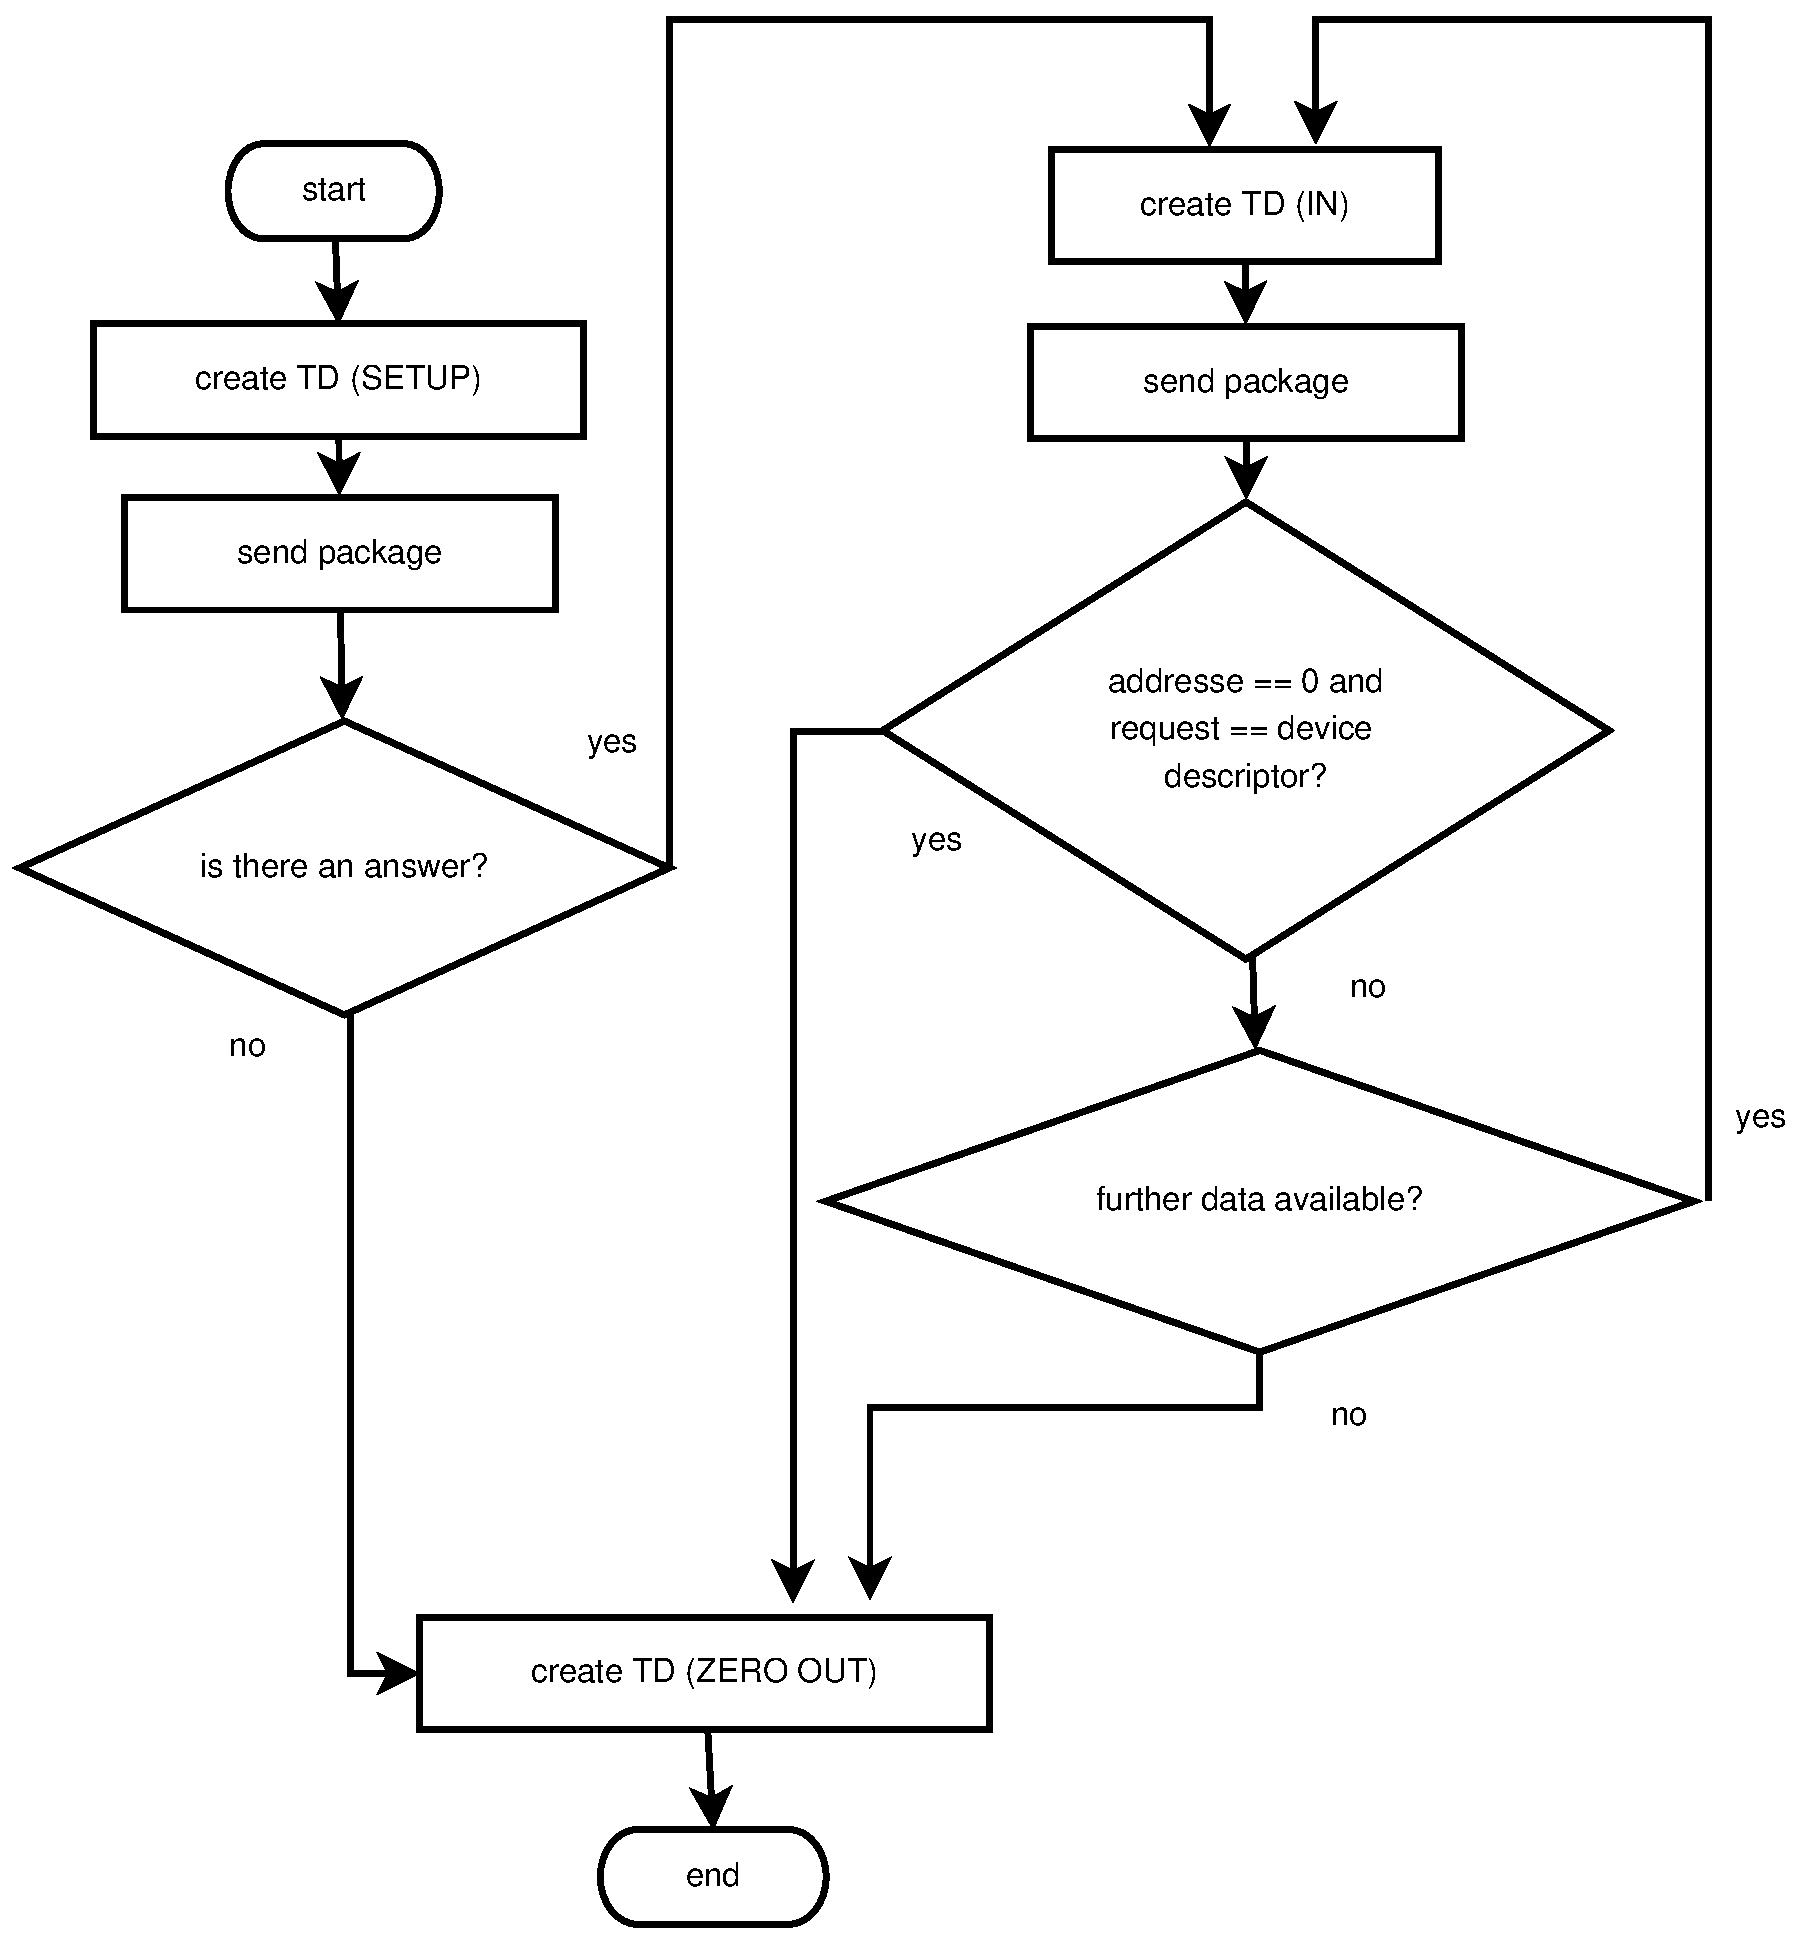
\includegraphics[width=12cm]{images/fluss_control}
\caption{Subdivision of a control transfer into transfer descriptors}
\label{fluss_control}
}
\end{figure}




\section{Integration in an own project}\label{integration}

In the following manual is described step by step how to integrate the USB stack in an existing or new project.
\newline\newline

\textbf{Step 1. Copy the USB directories} \newline
\newline
At first, the entire directories \textbf{core}, \textbf{lib} and \textbf{usbspec} are to be copied from the
USB stack archive to the own project directory.
If an own subfolder shall be created for the USB stack, the directories have to be copied
correspondingly to this folder.
\newline

\textbf{Step 2. Choose the host driver} \newline
\newline
In the next step a folder \textbf{host} is to be created on the same level as the folders in step 1.
In this folder a matching USB host controller driver has to be chosen from the archive and has to be copied to it.
For the compilation, the file \textbf{host.h} is also needed, thatswhy it has to be copied there aswell.
Many times, a driver needs additional files, for example the SL811HS driver.
There is another \textbf{sl811hs.h} file, that needs to be copied aswell.
If the host controller isn't integrated in the microprocessor, the connection and the transfer between microcontroller
and host controller is to be described, too.
In this case, the host controller provides own functions that, however, have to be adjusted.
How the connection is executed exactly has to be learned from the documentation of the host controller driver.
For the SL811HS this is described in chapter 8 of the diploma thesis.
\newline

\textbf{Step 3. Choose the drivers and the libraries }\newline
\newline
Exactly like the host driver, the necessary device drivers and libraries have to be copied in the created directory.
It is recommended to create the directory structure exactly as in the USB stack archive.
\begin{itemize}
\item drivers 
  \begin{itemize}
    \item class  
    \item net
    \item ...
  \end{itemize}
\item uclibusb
\end{itemize}

There are some folders, which are empty in the USB stack archive. Hopefully, after some time the collections grows bigger
and bigger.
\newline

\textbf{Step 4. Integrate the source codes in the compilation process} \newline
\newline
In the next step, the files have to be integrated in the compilation process of the project.
The directory including the USB stack files are to be given as include path, so that the compiler finds the
needed header files.
The command for the gcc would be \textit{gcc -I./}, or if there is an extra 
folder for the USB stack, \textit{gcc -I./foldertothestack}.
With the pre-processor flag DEBUG the debug mode can be switched on and off 
(\textit{gcc -DDEBUG=1} oder \textit{gcc -DDEBUG=0}).
\newline

\textbf{Step 5. Implementing the USB stack} \newline
The main function calls are shown in listing \ref{lst:usb_sample}.
In lines 1-4 the most important header files are integrated.
Which ones are to stand there depends on the drivers that are needed for the application.
The USB stack is initialized with the function call in line 8
Again, depending on the needed drivers the initialization functions of the drivers have to be called (lines 10-11).
For management and control tasks the USB stack has to be called regularly.
This can be solved with an infinite loop (line 13), or with a periodic timer of a thread library, etc.
If no periodic transfers happen and if the USB devices aren't changed during the operation,
periodic function calls can be foregone.

\lstset{language=C}
\begin{lstlisting}[caption={Implementing the USB stack},label={lst:usb_sample},
captionpos=b,
numbers=left,
basicstyle=\ttfamily\fontsize{10}{12}\selectfont,
commentstyle=\fontsize{10}{12}\selectfont]
#include <core/core.h>
#include <host/host.h>
#include <drivers/class/hub.h>
#include <drivers/class/storage.h>

int main(void)
{
  usb_init();

  usb_hub_init();
  usb_storage_init();
  
  while(1){
    usb_periodic(); 
    wait_ms(1);
  }
  return 0;
}
\end{lstlisting}

\textbf{Step 6.  Writing USB programs} \newline
The basis is now established and the programming of an USB application can be started.
A communication with an USB device, controlled directly by the functions of the USBDI may look like this:

\lstset{language=C}
\begin{lstlisting}[caption={Example of an USB program},label={lst:usb_driver_999},
captionpos=b,
numbers=left,
basicstyle=\ttfamily\fontsize{10}{12}\selectfont,
commentstyle=\fontsize{10}{12}\selectfont]
/* Pointer to the device data structure */
usb_device * dev = NULL;
char buf[] = {'A','B','C'};

/* Open USB connection to the device */
dev = usb_open(0x1234,0x5678);

/* Send data to the endpoint */
usb_bulk_write(dev,2,buf,3,1000);

/* Read data from the endpoint */
usb_bulk_read(dev,1,buf,3,1000);

/* Close connection */
usb_close(dev);

\end{lstlisting}
\index{Beispielprogramm}

%\section{Portierung auf eine neue Architektur}

%datentypen

%port leitungen fuer die hostcontroller treiber



%\section{USB Debug Monitor}
%\subsection{Integration in USB Host Stack}
%\subsection{Datenverkehr aufzeichnen}



	\chapter{Implementierung des USB-Host-Controller-Treibers f�r den SL811HS}

Ziel dieses Kapitels ist es, den Entwurfsprozess eines Host-Treibers
anhand des eingesetzten Bausteins SL811HS zu erl�utern.

\section{Der Baustein SL811HS}

\index{SL811HS}
Die Struktur und die technischen Daten �ber den SL811HS k�nnen 
in Kapitel \ref{kap:sl811} auf Seite \pageref{kap:sl811} nachgelesen werden.
In diesem Abschnitt werden die Details, 
die f�r die Programmierung des Treibers wichtig sind, angesprochen.

\subsubsection{Interrupt-Controller}

Der SL811HS \index{SL811HS} Interrupt-Controller verf�gt �ber eine
nach au�en gef�hrte Interrupt-Leitung (INTRQ), die bei verschiedenen
Ereignissen �ber interne Register aktiviert werden kann.
�ber ein Statusregister kann ermittelt werden, welche
Ereignisse ausgel�st worden sind.
Das Statusregister kann zur�ckgesetzt werden,
indem ein schreibender Zugriff auf das Register
ausgef�hrt wird.

\subsubsection{Speicher- und Register�bersicht}

Der SL811HS enth�lt 256 Bytes internen Speicher (siehe Abbildung \ref{sl811hs_ram}) f�r
den USB-Datenspeicher und die Control- bzw. Statusregister.
Im Host-Modus werden die ersten 16 Byte als Register
und die restlichen 240 Byte f�r die USB-Daten�bertragung
genutzt. Angesprochen wird der Speicher direkt
�ber die 8-Bit breite Busschnittstelle.

\begin{figure}[h]
{
\centering
\includegraphics[width=5cm]{images/sl811hs_ram}
\caption{Speicherkarte des SL811HS}
\label{sl811hs_ram}
}
\end{figure}

\section{Anbindung an einen Mikrocontroller}

Um den Treiber flexibel und unabh�ngig von den verbundenen I/O Leitungen an den verschiedensten Mikrocontrollern
einsetzen zu k�nnen,
wurde eine extra Ebene (siehe Abbildung \ref{sl811hs_io}) daf�r eingef�hrt. 
Die Funktionen (siehe Tabelle \ref{sl811hs_func}) der zus�tzlichen Ebene
befinden sich in den Dateien \textbf{sl811hs-io.c} und \textbf{sl811hs-io.h},
welche 
sich absichtlich nicht im Host-Ordner, sondern in dem Ordner
der Anwendung, die den Stack nutzt, befinden.
Die Konfiguration ist von der Anwendung und der Plattform, auf der entwickelt wird, abh�ngig.

\begin{figure}[h]
{
\centering
\includegraphics[width=10cm]{images/sl811hs_io}
\caption{Zugriffsfunktionen f�r SL811HS}
\label{sl811hs_io}
}
\end{figure}

\begin{table}[h]
\center
\begin{tabular}{|l|l|}
\hline
\rowcolor{Gray}[0.9\tabcolsep]
Funktion & Aufgabe\\ \hline
void sl811\_init() & Initialisierung der I/O-Leitungen\\ \hline
void sl811\_reset() & Reset des SL811HS durchf�hren\\ \hline
void sl811\_write(u8 addr, u8 data) & Byte an angegebene Adresse schreiben\\ \hline
u8 sl811\_read(u8 addr) & Byte an angegebener Adresse lesen\\ \hline
void sl811\_write\_burst(u8 data) & Bytes hintereinander schreiben\\ \hline
u8 sl811\_read\_burst() & Bytes hintereinander lesen\\ \hline
void sl811\_write\_buf(u8 addr, char *buf, u16 size) & Speicherbereich schreiben\\ \hline
void sl811\_read\_buf(u8 addr, char *buf, u16 size) & Speicherbereich lesen\\ \hline
\end{tabular}
\caption{Zugriffsfunktionen f�r SL811HS [sl811hs-io.h]}
\label{sl811hs_func}
\end{table}
\index{Zugriffsfunktionen f�r SL811HS}
\newpage
\section{Root-Hub-Treiber} \label{kap:roothub}
\index{Root-Hub-Treiber}
Die Funktionen f�r den Root-Hub-Treiber befinden sich mit unter in der Datei \textit{sl811hs-hcd.c}.
In den folgenden Listings wird auf die Implementierung der Funktionen eingegangen.
Der komplette Quelltext befindet sich im Host-Verzeichnis des USB-Stack-Archivs.
\newline\newline
Bekannterma�en ist der Root-Hub kein eigenes physikalisches USB-Ger�t,
sondern eine feste Einheit im Host-Controller. Im Gegensatz zu einem
externen USB-Hub wird der Status �ber die angesteckten USB-Ger�te am Hub
nicht �ber Endpunkte signalisiert, sondern �ber interne Register und Signale.
Dies sind die Aufgaben der Funktionen des Root-Hub-Treibers. Es m�ssen
die entsprechenden Register und Signale beobachtet und
neue und entfernte Ger�te dem USB-Stack gemeldet werden. 
\newline\newline
Wie jeder Ger�te- bzw. Klassen-Treiber ben�tigt auch der Root-Hub eine USB-Treiberdatenstrukur,
um sich am USB-Stack registrieren zu k�nnen.
\vskip 10pt  
\lstset{language=C}
\begin{lstlisting}[caption={SL811-Host-Controller-Treiber, sl811hs-hcd.c},label={sl811hs_rh},
name=roothub,
captionpos=b,
numbers=left,
firstline=1,
basicstyle=\ttfamily\fontsize{10}{12}\selectfont,
commentstyle=\fontsize{10}{12}\selectfont]
/* Treiberdatenstruktur */
usb_driver sl811_roothub = {
  .name   = "sl811_roothub",
  .probe  = sl811_roothub_probe,
  .check  = sl811_roothub_check,
  .data   = NULL,
};
\end{lstlisting}
\vskip 10pt  
Die \textit{probe} Funktion eines Treibers wird jedesmal
vom USB-Stack aufgerufen, wenn ein neues Ger�t am Bus
gefunden worden ist. In ihr wird �berpr�ft, ob das neue Ger�t von dem Treiber aus
angesteuert werden kann. Der Root-Hub-Treiber muss
diese �berpr�fung nicht durchf�hren, da der Host-Controller
einen Schritt zuvor schon ermittelt hat, ob der SL811-Baustein
verf�gbar ist. Ist dies der Fall, so ist
der Root-Hub ebenso verf�gbar, da er wie bereits beschrieben
eine feste Einheit im Host-Controller ist. Daher kann 
die Funktion \textit{sl811\_roothub\_probe} leer bleiben.
\vskip 10pt  
\begin{lstlisting}[caption={sl811\_roothub\_probe(), sl811hs-hcd.c},label={sl811hs_rh},
captionpos=b,
numbers=left,
name=roothub,
basicstyle=\ttfamily\fontsize{10}{12}\selectfont,
commentstyle=\fontsize{10}{12}\selectfont]
void sl811_roothub_probe()
{
  /* Root-Hub wurde bereits vom Host-Controller-Treiber erkannt */
}
\end{lstlisting}
\vskip 10pt  

Die �berwachung des abgehenden Ports am SL811-Host-Controller
wird in der Funktion \textit{sl811\_roothub\_check} vollzogen.
Die Funktionsweise wurde einem echten USB-Hub nachempfunden.
Bei einem USB-Hub existieren im Wesentlichen zwei Register. Im Ersten wird
der aktuelle Status angezeigt, d.h. ob sich im Moment ein Ger�t
an einem Port befindet. Im Zweiten ist ersichtlich,
ob ein Ger�t entfernt oder neu angesteckt wurde.
Mit Hilfe der Variable \textit{port\_change},
wird das Register f�r die �nderungen an dem Port nachgebildet.
Der Funktionsaufruf aus Zeile 19 entspricht dem ersten Register,
da hier der aktuelle Status des Ports abgefragt wird.


\vskip 10pt  
\begin{lstlisting}[caption={sl811\_roothub\_check(), sl811hs-hcd.c},label={sl811hs_rh},
captionpos=b,
numbers=left,
name=roothub,
showstringspaces=false,
basicstyle=\ttfamily\fontsize{10}{12}\selectfont,
commentstyle=\fontsize{10}{12}\selectfont]
void sl811_roothub_check()
{
  /* Ports �berwachen */
  // check for new device
  u16 *port_change = (u16*)sl811_roothub.data;

  // Status des Ports abfragen
  u8 status = sl811_read(SL811_ISR);
  // Signale zur�cksetzten
  sl811_write(SL811_ISR,SL811_ISR_DATA | SL811_ISR_SOFTIMER);

  // Entferne Ger�t gegebenenfalls
  if((status & SL811_ISR_RESET)) {  
    if(device_on_downstream!=NULL){
      #if USBMON
      core.stdout("Remove Device!\r\n");
      #endif
      usb_remove_device(device_on_downstream);
      device_on_downstream=NULL;
    }
    sl811_write(SL811_ISR,SL811_ISR_RESET);
  } 
\end{lstlisting}
\vskip 10pt  

Meldet der Root-Hub ein neues Ger�t, so 
wird der Port f�r den USB-Betrieb konfiguriert.
Es wird unteranderem die Generierung der SOF-Pakete
gestartet, das Ger�t mit Hilfe des Resetsignals
dazu veranlasst die Adresse 0 anzunehmen 
und zum Schluss die Enumerierung f�r das
USB-Ger�t gestartet. Mit dem Aufruf der
Funktion \textit{usb\_add\_device} aus Zeile 56
wird das neue Ger�t desweiteren am USB-Stack angemeldet.
\vskip 10pt  
\begin{lstlisting}[caption={Root-Hub Funktionalit�t, sl811hs-hcd.c},label={sl811hs_rh},
captionpos=b,
numbers=left,
name=roothub,
showstringspaces=false,
basicstyle=\ttfamily\fontsize{10}{12}\selectfont,
commentstyle=\fontsize{10}{12}\selectfont]
  else {
    if((port_change[0] & HUB_PORTSTATUS_C_PORT_CONNECTION)){
      #if USBMON
      core.stdout("Find new Device!\r\n");
      #endif

      /* init sof currently for fullspeed  (datasheet page 11)*/
      sl811_write(SL811_CSOF,0xAE);
      sl811_write(SL811_DATA,0xE0);

      /* reset device that function can answer to address 0 */
      sl811_write(SL811_IER,0x00);
      sl811_write(SL811_CTRL,SL811_CTRL_ENABLESOF|SL811_CTRL_RESETENGINE);
      sl811_write(SL811_ISR,0xff);
      wait_ms(20);

      /* start SOF generation */
      sl811_write(SL811_CTRL,SL811_CTRL_ENABLESOF);
      sl811_write(SL811_ISR,0xff);
      sl811_write(SL811_E0BASE,SL811_EPCTRL_ARM);
      wait_ms(50);

      device_on_downstream = usb_add_device();
      port_change[0]=0x00;
    }
  }
\end{lstlisting}
\vskip 10pt  

In den Zeilen 60-63 wird die Variable \textit{port\_change} f�r die �nderungen
abh�ngig vom abgefragten Ergebnis der Register des SL811HS
neu gesetzt.

\vskip 10pt  
\begin{lstlisting}[caption={port\_change, sl811hs-hcd.c},label={sl811hs_rh},
captionpos=b,
numbers=left,
name=roothub,
basicstyle=\ttfamily\fontsize{10}{12}\selectfont,
commentstyle=\fontsize{10}{12}\selectfont]
  if((status & SL811_ISR_INSERT)){
    port_change[0] |= HUB_PORTSTATUS_C_PORT_CONNECTION;
    sl811_write(SL811_ISR,SL811_ISR_INSERT);
  }
}
\end{lstlisting}
\vskip 10pt  


\section{Transfer-Deskriptoren-�bertragungsstrategie}
\index{Transfer-Deskriptor}


Der SL811HS bietet alle Control- und Statusregister (siehe Tabelle \ref{sl811hs_register} auf Seite \pageref{sl811hs_register}) f�r
die �bertragung von USB-Paketen doppelt (Registerset A und B) an.
Dadurch kann die Bandbreite der USB-Verbindung
besser genutzt werden. Ist eine Transaktion
abgeschlossen wird �ber das Interruptstatusregister angezeigt,
welches Registerset wieder bereit f�r ein neues Paket ist.
\newline\newline
Im folgenden wird auf den Quelltext der Funktion \textit{sl811\_start\_transfer} eingegangen,
welche f�r die �bertragung der einzelnen Transfer-Deskriptoren zust�ndig ist.
Im Rahmen der Diplomarbeit wurde eine einfache Version ausgearbeitet,
in der nur ein Registerset ohne Interruptbetrieb genutzt wird. Dieser 
Modus wird auch Bibliotheksmodus (\glqq{}LIBMODE\grqq{}) genannt,
da man so den USB-Stack wie eine einfache Funktionssammlung nutzen
kann, ohne ihn fester in die eigene Anwendung integrieren zu m�ssen.
\newline\newline
Beginnend wird in Zeile 3 ein Zeiger auf einen Transferdeskriptor erstellt,
mit dem im weiteren Verlauf der Funktion gearbeitet werden kann.
In Zeile 6 erh�lt der Zeiger die Adresse auf den n�chsten zu �bertragende Transferdeskriptor. 
\vskip 10pt  
\begin{lstlisting}[caption={SL811 �bertragungsfunktion f�r Transferdeskriporen, sl811hs-hcd.c},label={sl811hs_td},
captionpos=b,
numbers=left,
name=transfer,
basicstyle=\ttfamily\fontsize{10}{12}\selectfont,
commentstyle=\fontsize{10}{12}\selectfont]
void sl811_start_transfer()
{
  usb_transfer_descriptor * td;
  #if LIBMODE
  /* W�hle n�chsten Transferdeskriptor */
  td = td_usba;
  /* Interruptsignale abschalten (im LIBMODUS) */
  sl811_write(SL811_IER,0x00);
  #endif
\end{lstlisting}
\vskip 10pt  
Unabh�ngig vom Pakettyp, welcher im Transferdeskriptor angegeben ist,  muss f�r die �bertragung die
Adresse des USB-Ger�tes, die Anzahl der zu �bertragenden
Bytes und die Startadresse der Daten angegeben werden.
\vskip 10pt  
\begin{lstlisting}[caption={Transfer unah�ngige Einstellungen},label={sl811hs_td},
captionpos=b,
numbers=left,
name=transfer,
basicstyle=\ttfamily\fontsize{10}{12}\selectfont,
commentstyle=\fontsize{10}{12}\selectfont]
  sl811_write(SL811_E0CONT,td->devaddress); /* Ger�teadresse */
  sl811_write(SL811_E0LEN,td->actlen);      /* Anzahl der Bytes */
  sl811_write(SL811_E0ADDR,cMemStart);      /* Adresse f�r Daten */
\end{lstlisting}
\vskip 10pt  
Im folgenden muss abh�ngig vom Pakettyp unterschiedlich vorgegangen werden.
Differenziert wird hier zwischen SETUP-, IN- und OUT-Paket. Wobei Daten
immer nach einem IN oder OUT Paket folgen. Handelt es sich um ein SETUP-Paket,
wird zuerst die Anfrage (Standard-, Hersteller- oder Klassenanfrage) in
den internen Speicher des SL811HS-Host-Controllers kopiert (Zeile 17).
In Zeile 20 und 23 wird der Paket-Typ, die Endpunktnummer und der Datenpakettyp
dem Host-Controller mitgeteilt. Anschliessend wird der Transfer gestartet
und der Transferdeskriptor als versendet markiert.
\vskip 10pt  
\begin{lstlisting}[caption={PID-Setup, sl811hs-hcd.c},label={sl811hs_td},
captionpos=b,
numbers=left,
name=transfer,
basicstyle=\ttfamily\fontsize{10}{12}\selectfont,
commentstyle=\fontsize{10}{12}\selectfont]
  switch(td->pid) {
    case USB_PID_SETUP:

      /* Kopiere Anfrage in internen SL811HS RAM */
      sl811_write_buf(cMemStart,(unsigned char *)td->buffer,td->actlen);

      /* set pid and ep */
      sl811_write(SL811_E0STAT,PID_SETUP|td->endpoint); 

      /* Sende Setup-Paket mit DATA0 */
      sl811_write(SL811_E0CTRL,DATA0_WR); 

      /* Warte auf ACK */
      #if LIBMODE
      while((sl811_read(SL811_ISR)&SL811_ISR_USBA)==0);
      #endif
      td->state = USB_TRANSFER_DESCR_SEND;

    break;
\end{lstlisting}
\vskip 10pt  
Werden Daten von einem USB-Ger�t empfangen, m�ssen IN-Pakete versendet werden.
Als Antwort auf ein IN-Paket erh�lt der Host-Controller die Daten vom USB-Ger�t.
In Zeile 35 wird dem Host-Controller der Pakettyp und die Endpunktadresse mitgeteilt.
Zus�tzlich muss das Togl-Bit entsprechend gesetzt werden, um den Datenfluss
zu erm�glichen.
\vskip 10pt  
\begin{lstlisting}[caption={PID-IN, sl811hs-hcd.c},label={sl811hs_td},
captionpos=b,
numbers=left,
name=transfer,
basicstyle=\ttfamily\fontsize{10}{12}\selectfont,
commentstyle=\fontsize{10}{12}\selectfont]
    case USB_PID_IN:
      
      /* Pakettyp und Endpunkt setzten */
      sl811_write(SL811_E0STAT,PID_IN|td->endpoint); 
      sl811_write(SL811_ISR,0xff);

      /* DATA0 oder DATA1 */
      if(td->togl)
	sl811_write(SL811_E0CTRL,DATA1_RD); 
      else
	sl811_write(SL811_E0CTRL,DATA0_RD);

      td->state = USB_TRANSFER_DESCR_SEND;

      /* Warte auf ACK */
      #if LIBMODE
      while((sl811_read(SL811_ISR)&SL811_ISR_USBA)==0);

      /* Empfangene Daten vom internen SL811HS-RAM lesen */
      sl811_read_buf(cMemStart,(unsigned char *)td->buffer,td->actlen);
      #endif

    break;
\end{lstlisting}
\vskip 10pt  
Ausgehende Daten werden mit OUT-Paketen an USB-Ger�te gesendet.
Der Ablauf zu den anderen Pakettypen unterscheidet
sich nur darin, dass zuvor die zu �bertragenden Daten
in den internen Speicher des SL811HS geschrieben werden m�ssen.
\vskip 10pt  
\begin{lstlisting}[caption={PID-OUT, sl811hs-hcd.c},label={sl811hs_td},
captionpos=b,
numbers=left,
name=transfer,
basicstyle=\ttfamily\fontsize{10}{12}\selectfont,
commentstyle=\fontsize{10}{12}\selectfont]
    case USB_PID_OUT:
      /* Schreibe zu �bertragende Daten in SL811HS-RAM */
      if(td->actlen>0)
	sl811_write_buf(cMemStart,(unsigned char *)td->buffer,td->actlen);
     
      /* Pakettyp und Endpunktadresse */
      sl811_write(SL811_E0STAT,PID_OUT|td->endpoint);
      
      /* DATA0 oder DATA1 */
      if(td->togl)
	sl811_write(SL811_E0CTRL,DATA1_WR);
      else
	sl811_write(SL811_E0CTRL,DATA0_WR);

      td->state = USB_TRANSFER_DESCR_SEND;

      /* Warte auf ACK */
      #if LIBMODE
      while((sl811_read(SL811_ISR)&SL811_ISR_USBA)==0);
      #endif
    break;
  }    
}
\end{lstlisting}

\begin{table}[h]
\center
\begin{tabular}{|c|l|l|}
\hline
\rowcolor{Gray}[0.9\tabcolsep]
Adr. & Schreibzugriff & Lesezugriff\\ \hline\hline
0x00 & USB-A Control & USB-A Control\\ \hline
0x01 & USB-A Address & USB-A Address\\ \hline
0x02 & USB-A Length & USB-A Length\\ \hline
0x03 & USB-A PID/EP & USB-A Status\\ \hline
0x04 & USB-A Address & USB-A Count\\ \hline\hline
0x05 & Ctrl1 & Ctrl1\\ \hline
0x06 & Int. Enable & Int. Enable\\ \hline\hline
0x08 & USB-B Control & USB-B Control\\ \hline
0x09 & USB-B Address & USB-B Address\\ \hline
0x0A & USB-B Length & USB-B Length\\ \hline
0x0B & USB-B PID/EP & USB-B Status\\ \hline
0x0C & USB-B Address & USB-B Count\\ \hline\hline
0x0D & Int. Status & Int. Status \\ \hline
0x0E & SOF Low & HW Revision \\ \hline
0x0F & SOF High/Ctr2  & SOF High/Ctr2 \\ \hline
\end{tabular}
\caption{SL811HS Register�bersicht}
\label{sl811hs_register}
\end{table}


	\chapter{Implementierung der USB-Bibliotheken und -Ger�tetreiber}

Die wichtigsten Komponenten des USB-Stacks sind die Treiber und Bibliotheken der USB-Ger�te.
Mit ihnen kann eine abstrahierte Schnittstelle
f�r die Funktionen der einzelnen Ger�te angeboten werden.
Da die Treiber und Bibliotheken mit den Funktionen des USB-Stacks arbeiten
und nicht direkt mit den Host-Controllern kommunizieren,
k�nnen diese unabh�ngig vom eingesetzten Host-Controller
verwendet werden.
\newline\newline
Wie bereits erw�hnt, gibt es zwei Arten f�r die Ansteuerung 
eines USB-Ger�ts, Bibliotheken oder Treiber. Bibliotheken bieten sich vor allem f�r 
einfache Ger�te an, die �ber keine periodischen Endpunkte (wie Interrupt und Isochrone)
verf�gen. Soll ein USB-Ger�t hingegen von mehreren parallelen 
Programmpfaden aus angesprochen werden, so ist die Wahl eines Treibers die bessere M�glichkeit.
Der Treiber,
der die Zugriffszeiten gerecht auf alle Prozesse verteilen kann, dient als Schnittstelle zum Ger�t.
Abh�ngig vom Ger�t kann in den Treibern eigens der Mehrfachzugriff gesteuert werden.
\newline\newline
In den Treibern und Bibliotheken werden f�r die Kommunikation
und Steuerung der Verbindung die Funktionen des USB-Stacks verwendet (siehe Kapitel \ref{kap:usbdi} auf Seite \pageref{kap:usbdi}).
\newline\newline
Im n�chsten Abschnitt wird die Funktionsweise einer USB-Ger�te-Bibliothek erkl�rt.

\section{Bibliotheken} \label{kap:bib}
\index{Bibliotheken}
Der gro�e Vorteil von Bibliotheken gegen�ber Treibern ist,
dass sie leicht in den Programmfluss eines Programms
integriert werden k�nnen. An der Stelle, an der die Information 
vom USB Ger�t ben�tigt wird, muss die daf�r vorgesehene Bibliotheksfunktion einfach eingef�gt werden.
Sobald die Funktion das Ergebnis ermittelt hat, setzt das Hauptprogramm
mit der Arbeit fort. Der Nachteil von Bibliotheken ist, dass kostbare Rechenzeit
beim Warten auf das Ergebnis verloren geht. Oft kann dies 
aber f�r die Einfachheit in Kauf genommen werden, falls die Rechenzeit nicht anderweitig ben�tigt wird.
\newline\newline
Um eine Kommunikation mit einer Bibliothek durchf�hren zu k�nnen,
muss erst ein \glqq{}Handle\grqq{}\footnote{\label{foot:usbdi}\glqq{}Handle\grqq{} werden in der Informatik meist Zeiger auf Dateien oder Ger�te genannt.} f�r das Ger�t
erstellt werden. Im USB-Stack ist ein Handle ein Zeiger auf die \textit{usb\_device} Struktur (siehe Listing \ref{lst:usb_dev_struct} auf Seite \pageref{lst:usb_dev_struct})
des ausgew�hlten Ger�tes. Das Handle kann auf drei verschiedene Arten angelegt werden.

\begin{enumerate}
\item Mit der Funktion \textit{usb\_open} kann das Ger�t �ber die Hersteller- und Produkt-ID gefunden werden.
\item �ber den Klassencode kann das Ger�t mit der Funktion \textit{usb\_open\_class} gefunden werden.
\item Werden spezielle Deskriptoren f�r die Auswahl des Ger�tes ben�tigt, so kann ebenso �ber die interne Ger�teliste des USB-Kerns iteriert
und entsprechend f�r jedes Ger�t die spezielle Information abgefragt werden.
\end{enumerate}

Hat man den Zeiger auf das gesuchte Ger�t erhalten, kann mit den Funktionen 
einer Bibliothek gearbeitet werden. 
\newline\newline
Im folgenden wird eine Bibliothek vorgestellt, die im Rahmen der Diplomarbeit entstanden ist.
Die Bibliotheken befinden sich im Ordner uclibusb des Softwarearchivs.

\subsection{USB zu RS232-Wandler: FT232}
\index{FT232}
\index{RS232}
\index{USB zu RS232-Wandler}
\subsubsection{Struktur und Arbeitsweise}
Der FT232AM bzw. dessen Nachfolger der FT232BM von FTDI ist
ein Umsetzer von USB-zu-TTL-RS232-Signalen. F�r die Leitung RX und TX
gibt es jeweils einen Bulk-Endpunkt. Schreibt man in den TX-Endpunkt,
so werden die Daten �ber den UART des FT232 ausgegeben. Liest man im Gegensatz
von dem RX-Endpunkt, so erh�lt man die �ber den UART empfangenen Daten.
Intern, wie in Abbildung \ref{ftdi} zu sehen ist, sind direkt nach den UART
Leitungen TX und RX kleine FIFOs als Zwischenpuffer f�r die
empfangenen und zu sendenden Daten vorhanden.

\begin{figure}[h]
{
\centering
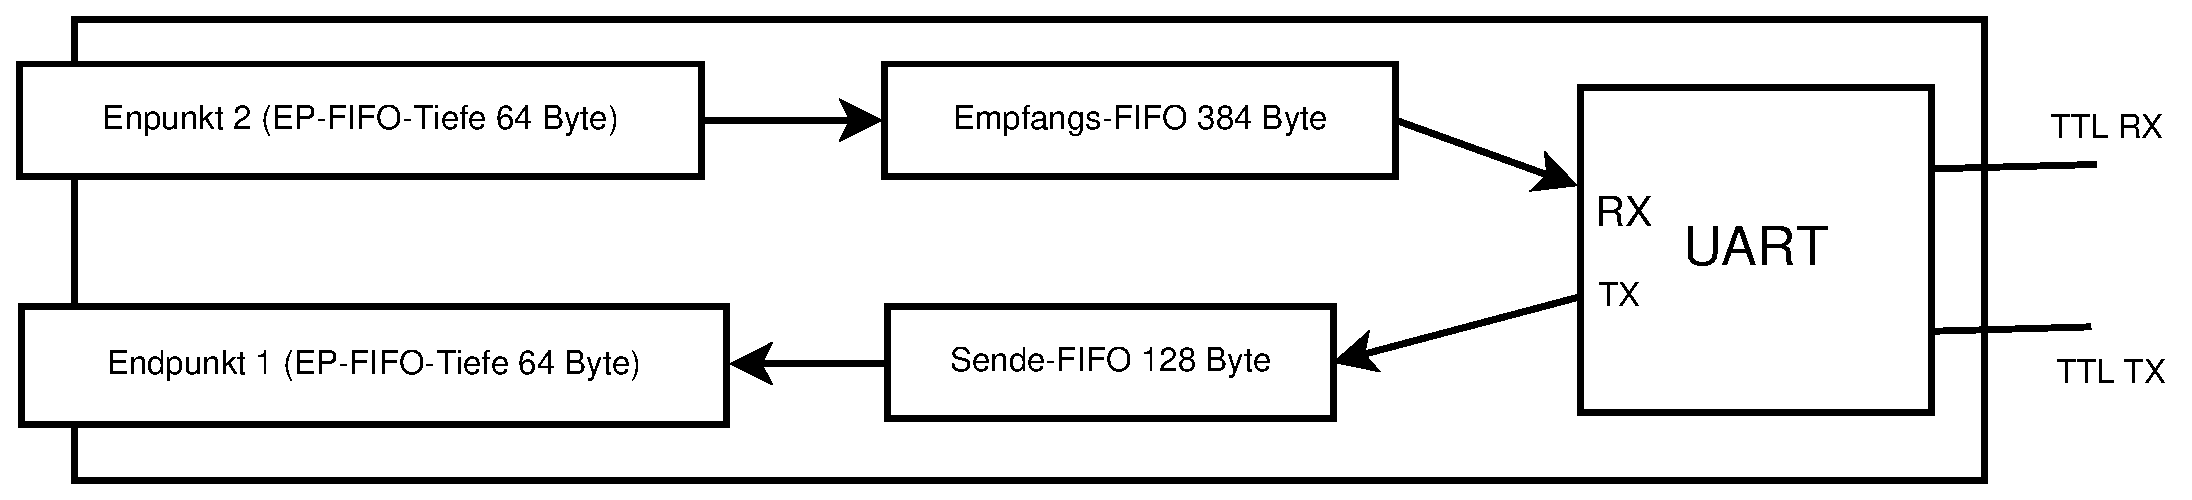
\includegraphics[width=15cm]{images/ftdi}
\caption{FT232-Struktur}
\label{ftdi}
}
\end{figure}

\newpage
\subsubsection{Konfiguration}

Der Hersteller FTDI bietet f�r die Konfiguration des Ger�tes
verschiedene Herstelleranfragen (engl. \glqq{}Vendor Requests\grqq{}, siehe Kapitel 2.15) an.
In Tabelle \ref{usb_ftdi} ist eine �bersicht der verschiedenen Anfragen dargestellt.

\begin{table}[h]
\center
\begin{tabular}{|l|l|l|}
\hline
\rowcolor{Gray}[0.9\tabcolsep]
Anfrage & Nr.& Beschreibung \\ \hline
FTDI\_SIO\_RESET  &0& L�st ein Reset des Ports aus \\ \hline
FTDI\_SIO\_MODEM\_CTRL &1& Modem-Controllregister beschreiben \\ \hline
FTDI\_SIO\_SET\_FLOW\_CTRL &2& Flusscontrollregister beschreiben\\ \hline
FTDI\_SIO\_SET\_BAUD\_RATE &3& �bertragungsrate einstellen\\ \hline
FTDI\_SIO\_SET\_DATA &4& Die Eigenschaft des Ports definieren\\ \hline
FTDI\_SIO\_GET\_MODEM\_STATUS &5& Abfrage des Modem-Status-Registers \\ \hline
FTDI\_SIO\_SET\_EVENT\_CHAR &6& Steuerzeichen definieren\\ \hline
FTDI\_SIO\_SET\_ERROR\_CHAR &7& Fehlerzeichen definieren\\ \hline
FTDI\_SIO\_SET\_LATENCY\_TIMER &8& Latenzzeit einstellen\\ \hline
FTDI\_SIO\_GET\_LATENCY\_TIMER &9& Latenzzeit abfragen\\ \hline
\end{tabular}
\caption{Herstelleranfragen des FT232}
\label{usb_ftdi}
\end{table}
Die Anfragen werden auf die gleiche Weise wie Standardanfragen �ber den Endpunkt 0
an das Ger�t gesendet. Da es vom Hersteller FDTI keine �bersicht
der einzelnen Nachrichten gibt, wurden die Parameter dem
offenen Linux-Treiber ftdi\_sio.c \cite{kernel} entnommen.

\subsubsection{Bibliotheksfunktionen}
\begin{table}[h]
\center
\begin{tabular}{|l|l|}
\hline
\rowcolor{Gray}[0.9\tabcolsep]
Anfrage & Beschreibung \\ \hline
\text{usb\_device * usb\_ft232\_open()} &  �ffnen der Verbindung \\ \hline
\text{usb\_ft232\_close(usb\_device *dev)} &  Beenden der Verbindung \\ \hline
\text{usb\_ft232\_send(usb\_device *dev,char *bytes, u8 length)} &  Daten senden \\ \hline
\text{usb\_ft232\_receive(usb\_device *dev,char *bytes, u8 length)} &  Daten  empfangen\\ \hline
\end{tabular}
\caption{Bibliotheksfunktionen des FT232, ft232.h}
\label{usb_ftdi_api}
\end{table}

Befindet sich ein FT232-Baustein am Bus des USB-Stacks,
so kann mit der Funktion \textit{usb\_ft232\_open} das Handle
f�r eine Kommunikation geholt werden. Um Daten versenden zu k�nnen,
existiert die Funktion \textit{usb\_ft232\_send}, um Daten entsprechend
empfangen zu k�nnen die Funktion \textit{usb\_ft232\_receive}. Als Parameter erwarten
beide Funktionen einen Zeiger auf die Ger�tedatenstruktur des angeschlossenen FT232-Bausteins, einen Zeiger auf einen Speicherbereich,
der zum Versenden oder zum Empfangen reserviert ist und als letzter Parameter wird die Anzahl der zu sendenden 
oder zu empfangenden Daten erwartet. Wird das Ger�t f�r die Kommunikation nicht 
mehr ben�tigt, kann das Ger�t mit \textit{usb\_ft232\_close} wieder
freigegeben werden.



\section{Ger�te- und Klassentreiber}
\index{Ger�tetreiber}
\index{Klassentreiber}
\subsection{Treiberarten}
F�r USB-Ger�te gibt es zwei Treiberarten, die Ger�tetreiber
und die Klassentreiber. Ein Ger�tetreiber ist speziell
f�r eine bestimmte Hardware entwickelt worden. Kauft man ein solches Ger�t,
so muss der dazugeh�rige vom Hersteller mitgelieferte Treiber installiert werden.
\newline\newline
F�r Standardger�te wie M�use, Tastaturen, Drucker, Netzwerkkarten, etc.
wurden mit der USB-Spezifikation sogenannte USB-Klassen definiert.
Eine Klasse beschreibt eine Schnittstellenstruktur f�r
eine bestimmte Ger�teklasse. Das Ziel dieser Klassen ist,
dass auf dem Rechner keine speziellen Treiber mehr f�r
Standardger�te installiert werden m�ssen. Dies bedeutet
aber nicht, dass diese Ger�te keine Treiber mehr ben�tigen.
Die Betriebssysteme halten Standardtreiber daf�r vor.
Daher entf�llt die Installation f�r den Benutzer und
Hersteller von Standardperipherie m�ssen keine Treiber mehr entwickeln und
verteilen.
\newline\newline
Die bekanntesten Ger�teklassen werden in einzelnen Dokumenten
von der USB-Organisation beschrieben:
\index{Human-Interface-Devices}
\index{Audio-Device-Class}
\index{Communication-Class-Device}
\index{Mass-Storage-Device-Class}
\index{Printer-Device-Class}
\begin{itemize}
\item Human-Interface-Devices \cite{class_hid}
\item Audio-Device-Class \cite{class_audio}
\item Communication-Class-Device \cite{class_cdc}
\item Mass-Storage-Device-Class \cite{class_msd}
\item Printer-Device-Class \cite{class_print}
\end{itemize}

\subsection{Automatische Treiberauswahl f�r Ger�te}
Wie in Kapitel \ref{kap:usbdi_driver} auf Seite \pageref{kap:usbdi_driver}
bereits angesprochen, werden Ger�te- und Klassentreiber
mit einer Instanz der Datenstruktur \textit{usb\_driver} (siehe Listing \ref{lst:usb_driver} auf Seite \pageref{lst:usb_driver}) am USB Stack registriert.
Die Datenstruktur enth�lt Zeiger auf die folgenden Funktionen eines Treibers.

\begin{description}
\item [usb\_$<$treibername$>$\_probe:] 
Diese Funktion wird immer dann vom USB-Stack aus aufgerufen, wenn ein neues Ger�t
am Bus erkannt wird. Sie �berpr�ft, ob das neue
Ger�t mit dem Treiber angesteuert werden kann. Dies kann
mit den gleichen drei M�glichkeiten wie f�r Bibliotheken aus Kapitel \ref{kap:bib} auf Seite \pageref{kap:bib} herausgefunden werden.
Ist das Ger�t von dem Treiber ansteuerbar, kann die Funktion das Ger�t in die internen Datenstrukturen 
des Treibers aufnehmen.
\newline\newline
F�r die Klassentreiber gibt es extra Felder im Ger�te- und Interface-Deskriptor des USB-Ger�tes,
in denen ein Klassencode angegeben werden kann. Mit speziellen Unterklassencodes
und Protokollnummern kann das Ger�t noch genauer identifiziert werden.

\item [usb\_$<$treibername$>$\_check:]
Befindet sich mindestens ein aktives Ger�t in den internen Treiberdatenstrukturen,
so wird im regelm��igen Abstand von einer Millisekunde die Funktion $"$check$"$ aufgerufen.
In dieser Funktion k�nnen f�r periodische Transfers Daten �bertragen
oder Verwaltungs- und andere Steuerungsaufgaben durchgef�hrt werden.
\end{description}

Im Treiberverzeichnis des Stacks liegt die Vorlage \textit{skeleton.c} f�r
einen USB-Ger�te- bzw. -Klassentreiber.

\subsection{HID-Treiber}
\index{HID-Treiber}
Die Ger�teklasse HID (\glqq{}Human-Interface-Device\grqq{}) umfasst alle Eingabeger�te (Maus, Tastatur, Zeichenbrett, etc.)
f�r die Steuerung- bzw. Eingabe von Befehlen vom Benutzer.
Der hier entwickelte Treiber bietet die Unterst�tzung f�r eine einfache Maus und Tastatur an. 
\newline\newline
Im Rahmen
der Diplomarbeit ist nur die Struktur und noch kein funktionsf�higer Treiber entstanden.
Die Implementierung wird im Anschluss an die Diplomarbeit stattfinden.
Wie das Protokoll f�r ein HID-Ger�t genau aussieht kann der USB-Klassen-Definition \cite{class_hid}
entnommen werden.
\newline\newline
In Tabelle \ref{usb_hid_api} ist eine �bersicht �ber die ben�tigten Funktionen gegeben.
\newpage
\begin{table}[h]
\center
\begin{tabular}{|l|l|}
\hline
\rowcolor{Gray}[0.9\tabcolsep]
Funktion & Beschreibung \\ \hline
\text{void usb\_hid\_init()} &  Treiber anmelden \\ \hline
\text{void usb\_hid\_mouse\_xy(void * callback, u8 interval\_ms)} & Callback f�r Mausbewegung \\ \hline
\text{void usb\_hid\_mouse\_leftclick(void * callback)} &  Callback f�r Links-Klick \\ \hline
\text{void usb\_hid\_mouse\_rightclick(void * callback)} &  Callback f�r Rechts-Klick \\ \hline
\text{void usb\_hid\_keyboard\_read(char * buf)} &  Empfangene Daten lesen \\ \hline
\text{u16 usb\_hid\_keyboard\_reveived\_bytes()} &  Anzahl empfangener Daten \\ \hline
\text{u8 usb\_hid\_keyboard\_lock\_states()} &  Lock-Tasten-Status abfragen \\ \hline
\text{void usb\_hid\_keyboard\_callback(void * callback)} &  Callback f�r Eingaben \\ \hline
\end{tabular}
\caption{Treiberfunktionen der HID-Ger�teklasse, hid.h}
\label{usb_hid_api}
\end{table}
\index{hid.h}

\subsection{Hub-Treiber} \label{kap:hub}
\index{Hub-Treiber}

Der Hub-Treiber ist bei vielen USB-Stacks fest in den Kern integriert.
Da nicht jede Embedded-L�sung ein Hub-Ger�t ben�tigt,
wurde der Hub-Treiber als ein eigener Klassentreiber entwickelt und kann 
bei Bedarf leicht weggelassen werden.
\newline\newline
Der Hub-Treiber bietet nur die drei Standardfunktionen \textit{usb\_hub\_init()}, \textit{usb\_hub\_probe()} und \textit{usb\_hub\_check()} an.
Wurde der Hub-Treiber mit der Funktion \textit{usb\_hub\_init()} geladen,
arbeitet er automatisch im Hintergrund. Jedesmal, wenn ein neues Ger�t am
Bus hinter einem Hub angeschlossen wird, �bernimmt der Hub-Treiber die Aufrufe,
welche f�r den Kern des USB-Stack erledigt werden m�ssen. Im Rahmen der Diplomarbeit
wurde nur die Grundstruktur f�r den Treiber entwickelt. Im Treiberarchiv
befindet sich das Ger�st f�r den Hub-Treiber, welches noch fertig implementiert werden muss.
\newline\newline
Der grobe Ablauf im Hub-Treiber kann der Abbildung \ref{hub} entnommen werden.

\begin{figure}[h]
{
\centering
\includegraphics[width=14cm]{images/hub}
\caption{Hub-Treiber Ablauf}
\label{hub}
}
\end{figure}

\subsection{Massenspeichertreiber}
\index{Massenspeicher-Treiber}
Viele USB-Ger�te bieten ein Massenspeicher-Interface an,
da �ber dies ganz einfach standardisiert Daten ausgetauscht werden k�nnen.
F�r die Ansteuerung der Ger�te werden �ber USB SCSI-Kommandos versendet.
Das hat den gro�en Vorteil, dass leicht USB-Treiber f�r Ger�te
wie Festplatten, CD-Brenner, ZIP-Laufwerke, etc. geschrieben werden k�nnen,
da diese meist mit dem SCSI-Protokoll ansprechbar sind.
\newline\newline
Abbildung \ref{msdstruktur} (Seite \pageref{msdstruktur}) zeigt die Struktur f�r die Datenspeicherverwaltung. 
Auf der untersten Ebene befindet sich das Massenspeichermedium,
welches �ber SCSI-Kommandos angesteuert wird. Die SCSI-Kommandos
werden eingebettet in USB-Nachrichten zwischen USB-Host und -Ger�t
�bertragen. Der Massenspeichertreiber auf dem System des USB-Host
kann die USB-Nachrichten entgegennehmen und die SCSI-Kommandos
extrahieren. F�r den automatischen Aufbau
der SCSI-Kommandos bietet der Massenspeichertreiber Funktionen an.
Basierend auf den Funktionen kann ein Dateisystem aufgesetzt werden.

\begin{figure}[h]
{
\centering
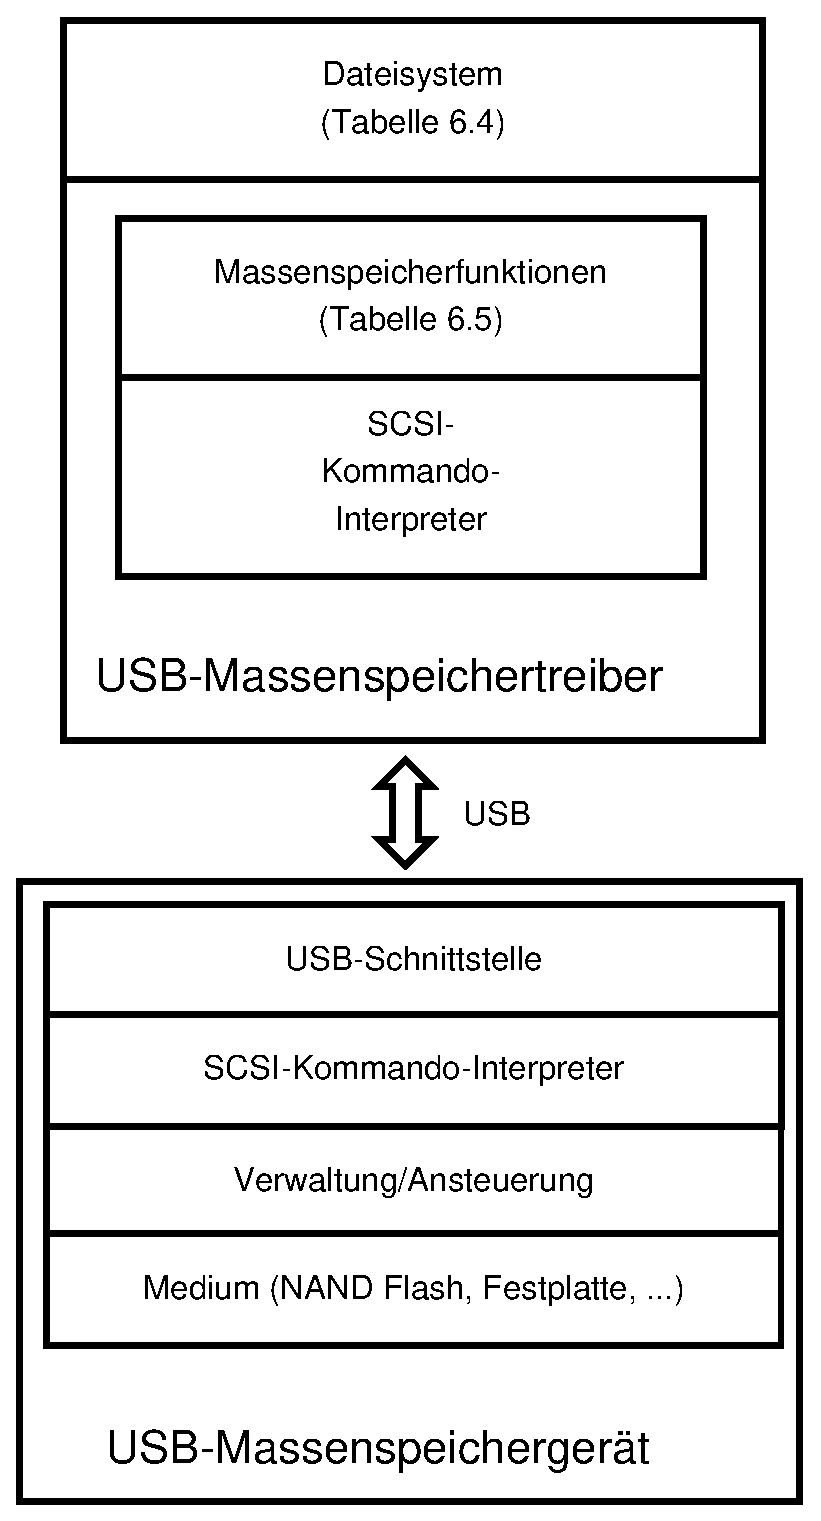
\includegraphics[height=11.5cm]{images/msdstruktur}
\caption{Struktur f�r die Datenspeicherverwaltung}
\label{msdstruktur}
}
\end{figure}

Im folgenden werden die Punkte aus der Abbildung \ref{msdstruktur} (Seite \pageref{msdstruktur})
von oben nach unten beschrieben.

\subsubsection{Embedded Dateisysteme}

Dateisysteme bieten M�glichkeiten f�r die 
Anordnung und den Zugriff auf Daten an.
Die ben�tigten Zugriffsfunktionen (siehe Tabelle \ref{usb_dateisystem_api} auf Seite \pageref{usb_dateisystem_api})
der verschiedenen Dateisysteme
unterscheiden sich, im Gegensatz zu der
Anordnung und den Strategien f�r die Verwaltung der Daten, meist wenig.
Abh�ngig vom eingesetzten Speichermedium und den Anforderungen
der Anwendungen muss das passende Dateisystem gew�hlt werden. Bei dem Entwurf
des Massenspeichertreibers muss darauf geachtet werden, dass m�glichst viele
Dateisysteme darauf aufbauen k�nnen.

\begin{table}[h]
\center
\begin{tabular}{|l|l|}
\hline
\rowcolor{Gray}[0.9\tabcolsep]
Funktion & Beschreibung \\ \hline
\text{mkdir} &  Erzeugen eines Verzeichnisses  \\ \hline
\text{chdir} &  Wechseln in ein anderes Verzeichnis \\ \hline
\text{rmdir} &  L�schen eines Verzeichnisses \\ \hline
\text{readdir} & Lesen von Verzeichniseintr�gen  \\ \hline
\text{open} & �ffnen einer Datei  \\ \hline
\text{close} & Schlie�en einer Datei  \\ \hline
\text{read} & Lesen einer Datei  \\ \hline
\text{write} & Schreiben einer Datei  \\ \hline
\text{unlink} & L�schen einer Datei  \\ \hline
\text{seek} & Positionieren des Lese- oder Schreibzeigers  \\ \hline
\end{tabular}
\caption{Ben�tigte Funktionen von Dateisystemen}
\label{usb_dateisystem_api}
\end{table}
\index{Dateisystem}


Es gibt eine Vielfalt an verschiedenen Dateisystemen f�r Embedded Systeme.
Die folgende Liste zeigt nur einen kleinen Auszug.

\begin{itemize}
\item \textbf{TINY File System} von Lucent Technologies (http://www.bell-labs.com/topic/swdist)
\item \textbf{Solid File System} von ELDOS (http://www.eldos.com/solfs/embedded.php)
\item \textbf{uc/Filesystem} von Embedded Office (http://www.embedded-office.de)
\item \textbf{FullFAT} von Holger Klabunde (http://www.holger-klabunde.de)
\item \textbf{FAT File System Module} von Elm Chan (http://elm-chan.org/)
\end{itemize}


\newpage
\subsubsection{Massenspeicherfunktionen}

Speichermedien wie Festplatten, USB-Sticks, CD-ROM Medien, etc.
haben gemeinsam, dass die Daten blockweise (ein Block entspricht einem Sektor) �bertragen und abgelegt werden.
F�r die Identifikation eines Speicherbereichs werden daher 
nicht Speicheradressen sondern Sektornummern ben�tigt.
Mit den
Funktionen aus der Tabelle \ref{usb_storage_api} kann
so abstrahiert auf viele Speichermedien zugegriffen werden.

\begin{table}[h]
\center
\begin{tabular}{|l|l|}
\hline
\rowcolor{Gray}[0.9\tabcolsep]
Funktion & Beschreibung \\ \hline
\text{void usb\_storage\_init()} &  Treiber anmelden \\ \hline
\text{u8 usb\_storage\_open(u8 device);} &  Verbindung �ffnen \\ \hline
\text{u8 usb\_storage\_read\_capacity(u8 device)} & Kapazit�t ermitteln \\ \hline
\text{u8 usb\_storage\_inquiry(u8 device)} &  Status abfragen \\ \hline
\text{void usb\_storage\_read\_sector(u8 device, u32 sector, char * buf)} &  Daten lesen \\ \hline
\text{void usb\_storage\_write\_sector(u8 device, u32 sector, char * buf)} &  Daten schreiben \\ \hline
\end{tabular}
\caption{Treiberfunktionen der Massenspeicher-Ger�teklasse, storage.h}
\label{usb_storage_api}
\end{table}
\index{storage.h}

\subsubsection{SCSI-Kommandointerpreter}

Wie bereits erw�hnt, werden USB-Massenspeicherger�te immer �ber
SCSI-Nachrichten, die �ber USB �bertragen werden, angesteuert.
Eine SCSI-Nachricht f�r ein USB-Massenspeicherger�t besteht aus zwei Paketen.
Das \glqq{}Command Block Wrapper CBW\grqq{}, das
die Anfrage enth�lt und das \glqq{}Command Status Wrapper CSW\grqq{},
das die Antwort bzw. den Status auf die Anfrage beinhaltet.
Die Datenstrukturen sind in den Listings \ref{lst:usb_cbw} und \ref{lst:usb_csw} abgedruckt.

\lstset{language=C}
\begin{lstlisting}[caption={Command Block Wrapper, storage.h},label={lst:usb_cbw},
captionpos=b,
basicstyle=\ttfamily\fontsize{10}{12}\selectfont,
commentstyle=\fontsize{10}{12}\selectfont]

typedef struct usb_storage_cbw_t usb_storage_cbw;
struct usb_storage_cbw_t {
  u32 dCBWSignature;  /* Signatur = 0x43425355 */
  u32 dCBWTag;
  u32 dCBWDataTransferLength;
  u8  bCWDFlags;      /* Enth�lt Bit f�r die Richtung */
  u8  bCBWLun;
  u8  bCBWCBLength;   /* 1 - 16 */
  u8  CBWCB[16];      /* SCSI Kommando */
};
\end{lstlisting}

\lstset{language=C}
\begin{lstlisting}[caption={Command Status Wrapper, storage.h},label={lst:usb_csw},
captionpos=b,
basicstyle=\ttfamily\fontsize{10}{12}\selectfont,
commentstyle=\fontsize{10}{12}\selectfont]

typedef struct usb_storage_csw_t usb_storage_csw;
struct usb_storage_csw_t {
  u32 dCSWSignature;	/* Signatur = 0x53425355 */
  u32 dCSWTag;		/* identisch mit dCBWTag aus Anfrage */
  u32 dCSWDataResidue;	/* identisch mit bCBWCBLength */
  u8  bCSWStatus;	/* Status �ber Erfolg */
};
\end{lstlisting}

Eingebettet in \glqq{}Command Block Wrapper CBW\grqq{} (Listing \ref{lst:usb_cbw})
werden die SCSI-Kommandos �bertragen. In der Tabelle \ref{usb_scsi} sind
die wichtigsten Kommandos aufgelistet. Der genaue Aufbau kann dem Dokument \cite{class_msd} entnommen werden.

\begin{table}[h]
\center
\begin{tabular}{|c|l|}
\hline
\rowcolor{Gray}[0.9\tabcolsep]
Kommando & Beschreibung \\ \hline
\text{0x00} & Test Unit Ready \\ \hline
\text{0x03} & Request Sense \\ \hline
\text{0x12} & Inquiry \\ \hline
\text{0x1A} & Mode Sense \\ \hline
\text{0x1E} & Prevent Allow Media Removal \\ \hline
\text{0x25} & Read Capacity \\ \hline
\text{0x28} & Read \\ \hline
\text{0x2A} & Write \\ \hline
\text{0x2F} & Verify \\ \hline
\end{tabular}
\caption{Typische SCSI-Kommandos, storage.h}
\label{usb_scsi}
\end{table}

Abbildung \ref{datenfluss_cbw} zeigt den Fluss f�r Befehle, eingehende und ausgehende Daten und den Status-Transport.

\begin{figure}[h]
{
\centering
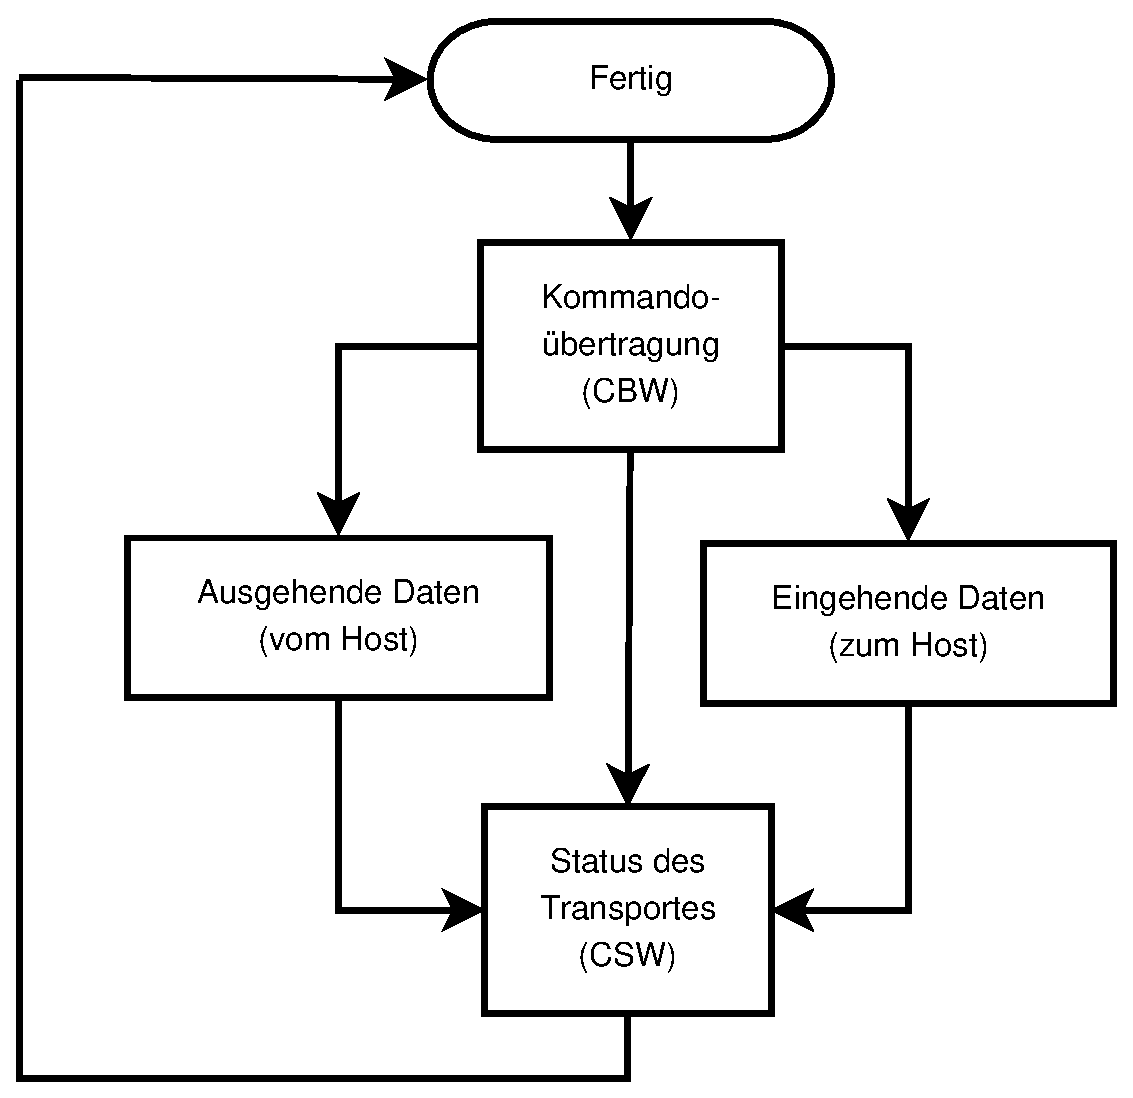
\includegraphics[height=8cm]{images/cbw_csw}
\caption{Datenfluss von CBW und CSW}
\label{datenfluss_cbw}
}
\end{figure}

Der Quelltext im Listing \ref{lst:usb_capacity} zeigt
die Implementierung der Funktion f�r das Abfragen der Speicherkapazit�t eines
Massenspeicherger�ts. Im Wesentlichen wird in Zeile 12 die Klassenanfrage \textit{Bulk-Only Mass Storage Reset}
an das Ger�t gesendet (mehr zu dieser Anfrage in Abschnitt \ref{bulk_reset} auf Seite \pageref{bulk_reset}).
Desweiteren wird der Command Block Wrapper mit dem SCSI-Kommando f�r die Abfrage der Kapazit�t 
aufgebaut und anschlie�end an das Ger�t gesendet. Als Antwort erh�lt man die Sektorgr�sse
und die Anzahl der Sektoren, woraus man sich wiederum die Kapazit�t durch Multiplikation
der beiden Faktoren ermitteln kann.

\lstset{language=C}
\begin{lstlisting}[caption={Abfrage der Speicherkapazit�t eines Massenpeicherger�ts, storage.c},label={lst:usb_capacity},
captionpos=b,
numbers=left,
basicstyle=\ttfamily\fontsize{10}{12}\selectfont,
commentstyle=\fontsize{10}{12}\selectfont]
u8 usb_storage_read_capacity(u8 device, char * size)
{
  /* send cwb "usbc" */
  char tmp[8];
  u8 i;
  u32 size;
  usb_storage_cbw  * cbw = (usb_storage_cbw*)malloc(sizeof(usb_storage_cbw));

  usb_control_msg(massstorage[device], 0x02,1,0, 0x8100, 0,tmp, 8, 0); 

  cbw->dCBWSignature= 0x43425355;
  cbw->dCWBTag=0x826A6008;
  cbw->dCBWDataTransferLength=0x00000008;
  cbw->bCWDFlags=0x80;
  cbw->bCBWLun=0x00;
  cbw->bCBWCBLength=0x0A;

  for(i=0;i<16;i++)
    cbw->CBWCB[i]=0x00;

  cbw->CBWCB[0]=0x25; // SCSI: Speicherkapazit�t abfragen

  usb_bulk_write(massstorage[device], 2, (char*)cbw, 31, 0);
  usb_bulk_read(massstorage[device], 1, (char*)cbw, 8, 0);
  
  /* Ersten 4 Byte = Max. Sector Adresse, zweiten 4 Byte = Sectorgr�sse */
  for(i=0;i<8;i++)
    size[i]=cbw[i];

  usb_bulk_read(massstorage[device], 1, (char*)cbw, 13, 0);

  free(cbw);

  return 0;
}
\end{lstlisting}





\subsubsection{USB-Schnittstelle}
Die USB-Klassenspezifikation f�r Massenspeicher bietet verschiedene Endpunkt-Konfigurationen
f�r den Betrieb an. Die einfachste und am meisten implementierte Konfiguration
ist die sogenannte \glqq{}Bulk-Only\grqq{} Methode. Hierbei werden die Daten
�ber einen eingehenden und ausgehenden Bulk-Endpunkt �bertragen.
Das Betriebssystem oder die Anwendung kann �ber den Klassencode 0x08 
und den Interface-Protokoll-Code 0x50 erkennen, dass es sich um ein Bulk-Only-Ger�t handelt.
\newline\newline
Au�erdem muss jedes Bulk-Only-Ger�t die folgenden beiden Klassen-Anfragen
beantworten k�nnen.
\label{bulk_reset}
\newline\newline
\textbf{Bulk-Only Mass Storage Reset}\newline\newline
Diese Anfrage wird ben�tigt, um das Massenspeicherger�t zu reseten. Nachfolgend
der Anfrage muss das Massenspeicherger�t auf ein Command-Block-Wrapper-Paket 
sofort antworten k�nnen. Um den Reset auszul�sen, muss die Anfrage wie folgt aufgebaut sein:
\begin{itemize}
\item \textit{bmRequestType:} Klasse, Interface, Host zu Ger�t
\item \textit{bRequest} 255 (0xFF)
\item \textit{wValue} 0
\item \textit{wIndex} Interface-Nummer
\item \textit{wLength} 0
\end{itemize}


\textbf{Get Max LUN}\newline\newline
In einem Massenspeicherger�t k�nnen mehrere logische Speicherbereiche
genutzt werden. �ber die sogenannte \glqq{}Logical-Unit-Number\grqq{}
kann ein Bereich ausgew�hlt werden. Mit der Klassen-Anfrage kann ermittelt
werden, wieviele dieser logischen Bereiche existieren.

\begin{itemize}
\item \textit{bmRequestType:} Klasse, Interface, Ger�t zu Host
\item \textit{bRequest} 254 (0xFE)
\item \textit{wValue} 0
\item \textit{wIndex} Interface-Nummer
\item \textit{wLength} 1 
\end{itemize}


\subsubsection{SCSI-Kommandointerpreter, Verwaltung/Ansteuerung, Medium}
Die letzten drei Ebenen werden unabh�ngig vom Treiber im USB-Ger�t
realisiert und sind daher f�r den Entwurf des Massenspeichertreibers
nicht von Bedeutung.






	
\chapter{Testplatine und Entwicklungsumgebung}
\index{Testplatine}
\index{Entwicklungsumgebung}
Im Rahmen der Diplomarbeit wurde eine Test- und Entwicklungsplatine f�r
die Entwicklung des USB-Stacks entworfen.

\section{Anforderungen an die Schaltung}

Prim�r dient die Schaltung dazu, die Funktionen des USB-Stacks mit USB-Ger�ten
�berpr�fen zu k�nnen. Da die Platine selbst ge�tzt und best�ckt werden sollte, wurde auf
den Einsatz von SMD-Bauteilen verzichtet.
\newline\newline
Folgende Anforderungen wurden an die Platine gestellt:

\begin{itemize}
\item Eine RS232-Schnittstelle f�r Statusmeldungen
\item Einfache Programmierm�glichkeit f�r den eingesetzten Mikrocontroller
\item Stromversorgung �ber ein USB-Kabel
\item Eine USB-Buchse f�r den USB-Port des Host-Controllers
\item Eine Leuchtdiode an einem I/O-Port f�r optische Statusmeldungen
\item Eine Layoutvorlage f�r einseitig beschichtete Platine ohne Durchkontaktierungen
\end{itemize}

\subsubsection{Eingesetzter Mikrocontroller}
Als Mikrocontroller wurde ein ATMega32 (8 Bit) der bekannten AVR-Reihe von Atmel gew�hlt.
Dieser ist preiswert zu erwerben und hat gen�gend Ports f�r die Anbindung eines
Host-Controllers. Weiterhin gibt es f�r die AVR-Controller-Reihe viele freie Programme
f�r die Softwareentwicklung.
\newline\newline
Technische Daten:
\begin{enumerate}
\item 32 KB Programmspeicher (Flash)
\item 2 KB Arbeitsspeicher (RAM) 
\item 1 KB Datenspeicher (EEPROM) 
\item Bei 16 MHz bis zu 16 MIPS\footnote{\label{foot:usbdi}\glqq{}Millionen Instruktionen pro Sekunde\grqq{} ist ein Ma� f�r die Leistungsf�higkeit von Prozessoren.}
\item 20 nach au�en gef�hrte I/O-Leitungen
\item 5 V Betriebs- und I/O-Spannung
\end{enumerate}
\subsubsection{Eingesetzter Host-Controller}
\index{SL811HS}
Ein einfacher und bew�hrter USB-Host-Controller ist der SL811HS von Cypress.
Da der SL811HS speziell f�r Embedded Systeme entwickelt worden ist,
kann er �ber eine einfache Standard-Bus-Schnittstelle angesteuert werden.
Der Controller kann in den Betriebsarten Host und Slave verwendet werden,
jedoch  ist f�r die vorliegende Diplomarbeit nur der Hostbetrieb interessant.
Den SL811HS gibt es in den Bauformen TQFP und PLCC. Das PLCC-Geh�use ist ideal
f�r Prototypen, da es f�r diese Bauform Sockel gibt, mit denen man den Controller
einfach austauschen kann.
\newline\newline
Die wichtigsten Eigenschaften des USB-Host-Controllers:
\begin{enumerate}
\item Kompatibel zur USB Spezifikation 1.1
\item Automatische Erkennung von \glqq{}Low-\grqq{} und \glqq{}Full-\grqq{} Speed-Ger�ten
\item 8-Bit bidirektionale Port-Schnittstelle
\item Integrierter Root-Hub
\item 256 Byte interner Speicher
\item 5 V-tolerante Portleitungen
\item Viele automatische Routinen f�r den USB-Betrieb wie z.B. SOF-Generierung, CRC5-Pr�fsummenerstellung, und andere. 
\end{enumerate}
\label{kap:sl811}

Das Blockdiagramm in Abbildung \ref{sl811hs} zeigt die interne Struktur im Host-Controller
Baustein SL811HS. Auf der linken Seite befindet sich der Root-Hub,
welcher die Schnittstelle zum USB-Kabel zu den Ger�ten ist. Direkt
nach dem Root-Hub befindet die SIE (\glqq{}Serial Interface Engine\grqq{})
welche die Daten entsprechend wie in Kapitel \ref{kap:signal} (Seite \pageref{kap:signal}) verarbeitet.
Die SIE ben�tigt f�r die Abtastung und die �bertragung der Daten einen konstanten Takt von 48 MHz, welcher
�ber den Taktgenerator zugef�hrt wird. Ebenfalls ben�tigt die SIE noch
die Information, ob der Baustein als Master oder Slave betrieben wird. Abh�ngig
von der gew�hlten Betriebsart werden desweiteren verschiedene Interrupts vom Interrupt-Controller
ausgel�st, weshalb eine Verbindung zwischen dem Master/Slave-Controller und dem Interrupt-Controller besteht. 
Die Prozessorschnittstelle auf der rechten Seite erm�glicht den Zugriff
auf die internen Register und den internen Speicher des SL811HS-Host-Controllers.

\begin{figure}[h]
{
\centering
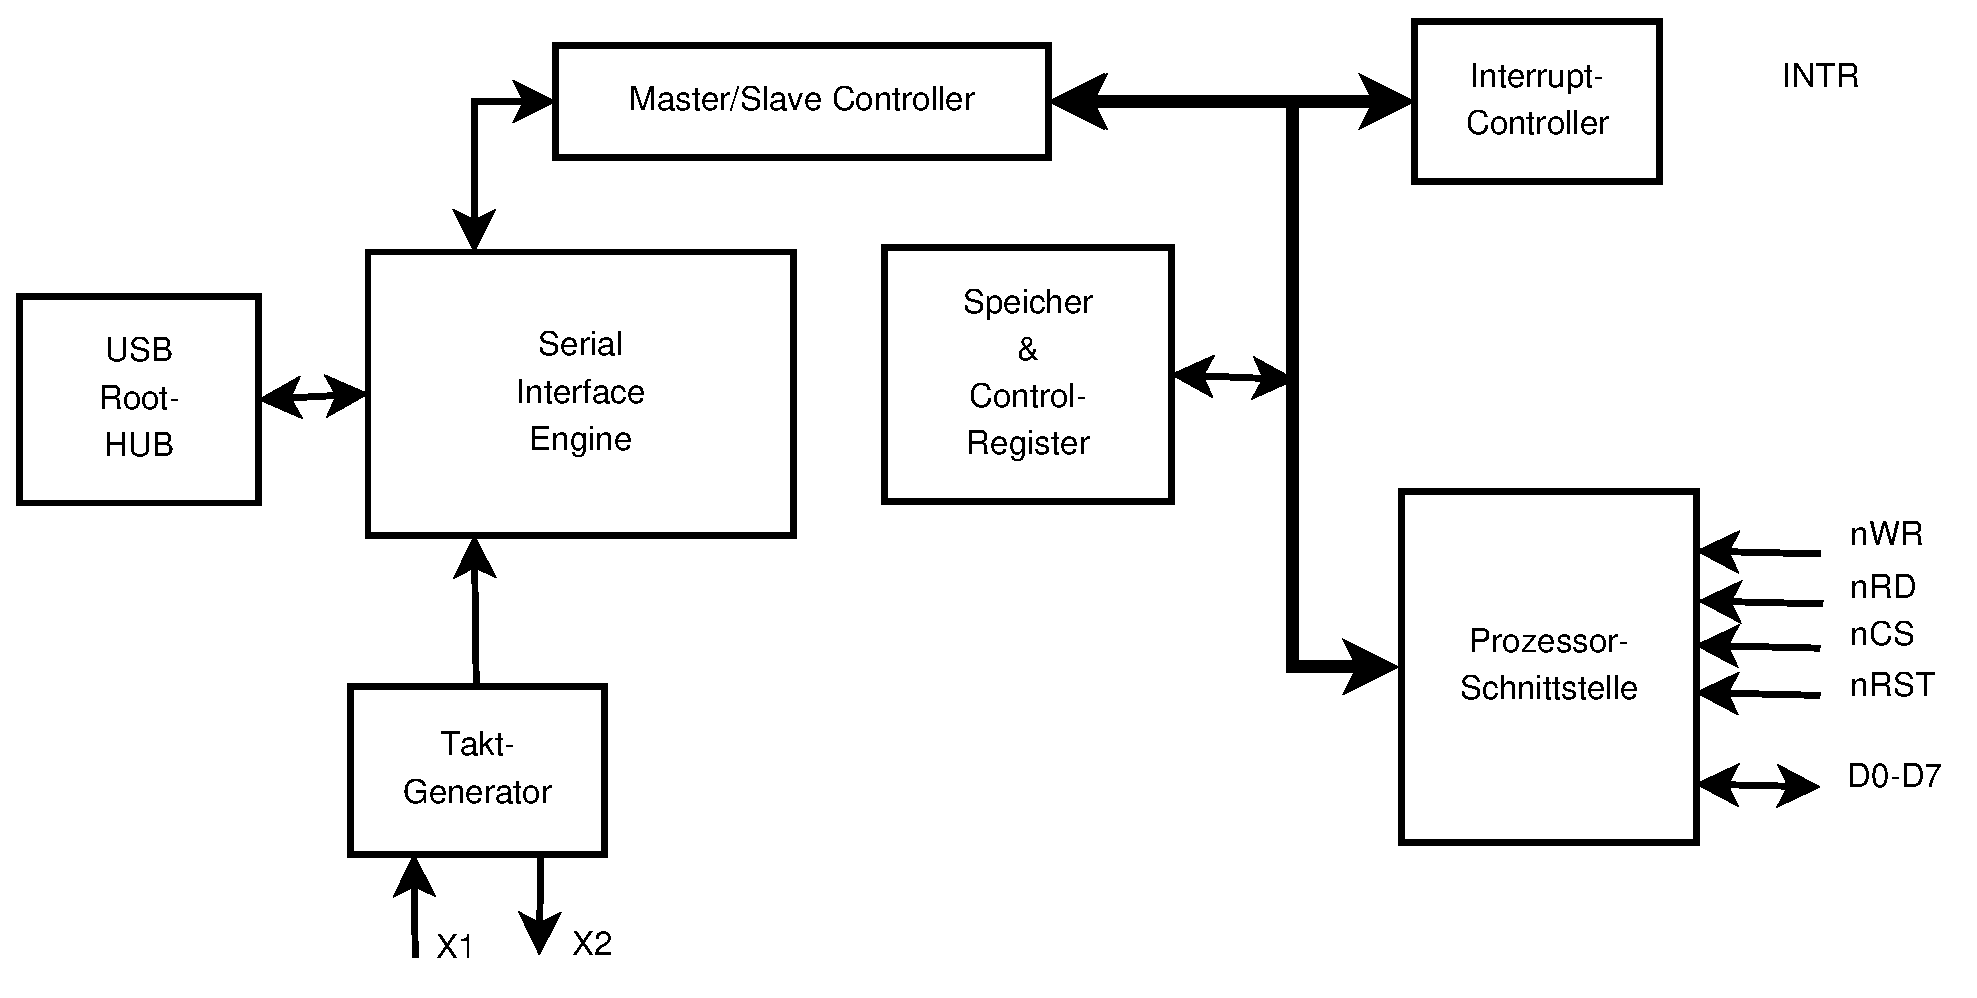
\includegraphics[width=14cm]{images/sl811hs_block}
\caption{Blockdiagramm SL811HS}
\label{sl811hs}
}
\end{figure}

\subsubsection{Entwurf der Schaltung}
Die Schaltung (siehe Abbildung \ref{schaltplan} auf Seite \pageref{schaltplan}) enth�lt nur die absolut notwendigen Bauteile. F�r die Stromversorgung
wurde die USB-Buchse X1 montiert. Dadurch kann die Testplatine �ber
ein einfaches USB-Kabel mit Strom von einem Computer versorgt werden.
Auf der Platine befinden sich der Host-Controller SL811HS,
ein RS232-Pegelwandler f�r Debugausgaben und der Mikrocontroller ATMega32 als Controller,
der die USB-Stack-Firmware ausf�hrt.
Da der SL811HS mit 3,3V versorgt werden muss, ist auf der Unterseite der Platine
ein Spannungsregler angebracht. Als Taktquelle ben�tigt
der Host-Controller entweder eine 12 MHz oder 48 MHz Taktquelle.
In der Schaltung wurde ein
externer 48 MHz Quarzoszillator eingebaut. Da der SL811HS sowohl
als Host-Controller als auch als USB-Ger�t eingesetzt werden kann, ist darauf
zu achten, dass die Signalleitung M/S (\glqq{}Pin Master/Slave Select\grqq{}) entsprechend richtig konfiguriert wird.
Der Mikrocontroller wird ebenfalls mit einem externen 16 MHz Quarz versorgt.
%Es besteht
%die M�glichkeit, auch einen internen Oszillator zu aktivieren.
%Da dieser aber nicht so genau ist, wurde auf einen externen zur�ckgegriffen.
\newline\newline
In Abbildung \ref{bestueckung} ist der Best�ckungsplan und das
Layout der Platine abgedruckt.
\begin{figure}[hpt]
{
\centering
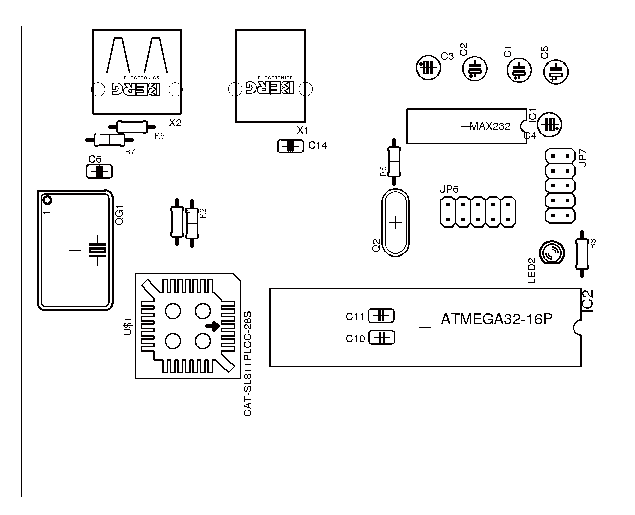
\includegraphics{images/bestueckung}
\hfill
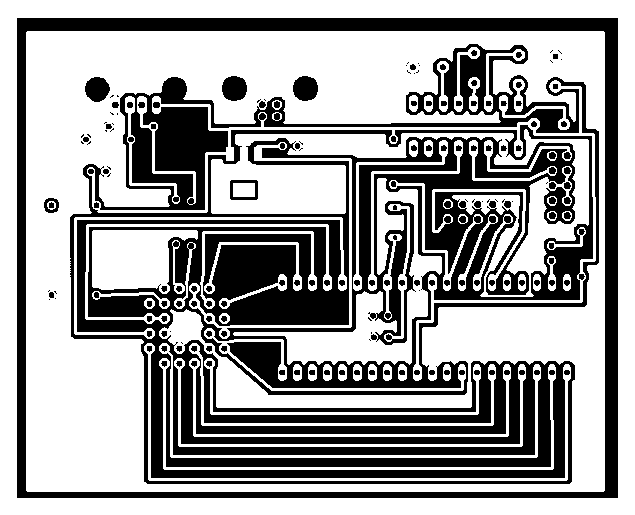
\includegraphics{images/layout}
\caption{Best�ckungsplan und Layout der Platine}
\label{bestueckung}
}
\end{figure}

%\begin{figure}[h]
%{
%\centering
%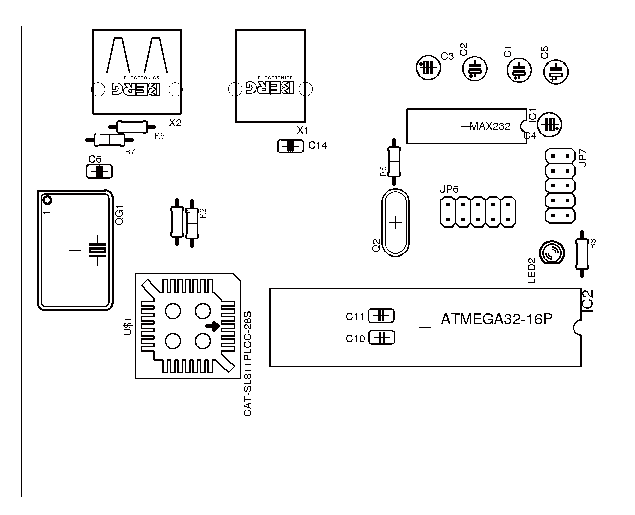
\includegraphics[height=7cm]{images/bestueckung}
%\caption{Best�ckungsplan der Testplatine}
%\label{bestueckung}
%}
%\end{figure}

%\begin{figure}[h]
%{
%\centering
%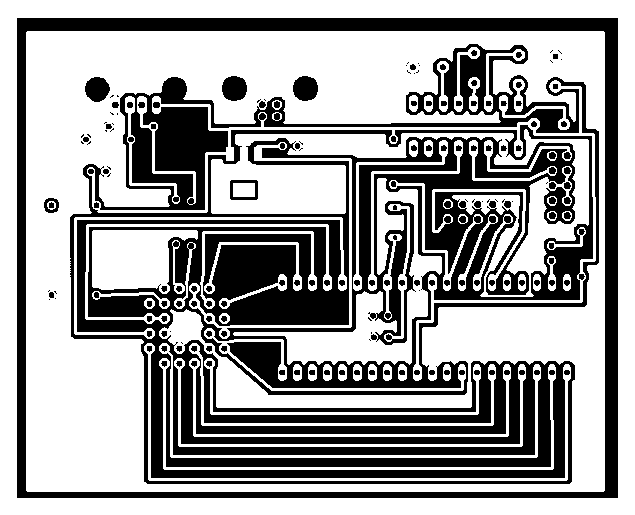
\includegraphics[height=7cm]{images/layout}
%\caption{Layout der Testplatine}
%\label{layout}
%}
%\end{figure}
%\newpage


\section{Entwicklungsumgebung}
Da die Diplomarbeit ein Open-Source-Projekt werden soll,
wurde bei der Entwicklung darauf geachtet, dass nur mit
freien oder zumindest kostenlosen Programmen gearbeitet wurde.
\newline\newline
Der Entwicklungsaufbau sah wie in Abbildung \ref{entwicklung} dargestellt aus.
Der Computer, der als Entwicklungsplattform dient, 
ist mit der Testplatine �ber ein RS232- und einem USB-Kabel f�r die Stromversorgung 
verbunden. Programmiert wird der Mikrocontroller ATMega32 �ber einen extra USB-Adapter \cite{usbprog}.
Der USB-Port ist die Schnittstelle f�r USB-Ger�te f�r die Treiberentwicklung zum Software-Stack hin.
\begin{figure}[h]
{
\centering
\includegraphics[width=14cm]{images/entwicklung}
\caption{Entwicklungsumgebung}
\label{entwicklung}
}
\end{figure}
\newline\newline
F�r die Hardwareentwicklung wurden folgende Programme und Ger�te verwendet:

\begin{itemize}
\item Eagle v. 3.5\cite{eagle}, Freeware, zum Zeichnen des Schaltplans und Setzen des Layouts f�r die Platine.
\item avrdude\cite{avrdude}, Open-Source, f�r die Programmierung des Mikrocontrollers.
\item usbprog\cite{usbprog}, Open-Source-Hardware, Programmieradapter f�r AVR Mikrocontroller.
\end{itemize}

F�r die Software kamen folgende Programme zum Einsatz:

\begin{itemize}
\item GCC f�r Linux Version 4.1.0\cite{gcc}, Open-Source, freier C Compiler.
\item Kermit\cite{kermit}, Open-Source, Terminal (wurde f�r die Debugausgaben �ber RS232 ben�tigt).
\end{itemize}

Die Liste der zur Verf�gung stehenden USB-Ger�te w�hrend des Entwurfs:

\begin{itemize}
\item \glqq{}Hi-Speed USB 2.0\grqq{} Hub von equip.
\item \glqq{}USB-Modul UM100 (FT232AM)\grqq{} von ELV.
\item \glqq{}MP3-Player Lyra\grqq{} von Thomson (als Massenspeicher).
\item \glqq{}1 GB USB Flash Speicher Stick\grqq{} von PNY.
\item \glqq{}AVR JTAGICE mk2\grqq{} von Atmel.
\item \glqq{}E232 Drucker\grqq{} von Lexmark.
\end{itemize}

Die Vielfalt war vor allem f�r das Testen der Enumerierung sehr wichtig.

\begin{figure}
{
\centering
\includegraphics[scale=0.7]{schaltplan.ps}
\caption{Schaltplan der Testplatine}
\label{schaltplan}
}
\end{figure}


	\chapter{Fazit und Ausblick}
\section{Fazit}
Ziel der Diplomarbeit war es, einen freien, portablen
und erweiterbaren USB-Host-Stack f�r Embedded-Systeme zu entwickeln.
Um einen einfach einsetzbaren und vollst�ndigen USB-Host-Stack
erstellen zu k�nnen, musste viel Arbeit in das Design der Softwarestruktur investiert werden.
Denn nur mit einer klaren und �bersichtlichen Struktur k�nnen andere
Entwickler daf�r begeistert werden, diesen USB-Stack zu nutzen.
Die klare Struktur wurde mit einer Aufteilung in einzelne Komponenten
und Treiber erreicht. F�r den USB-Host-Stack wurden in der Diplomarbeit
ein Host-Controller-Treiber f�r den Baustein SL811HS von Cypress, 
ein USB-Ger�tetreiber f�r den USB zu RS232 Wandler FT232 von FTDI Inc.
und USB-Klassentreiber f�r Massenspeicher, Hub- und HID-Ger�te entwickelt.
\newline\newline
Mit Hilfe von Beispielanwendungen wird dem Anwender
der Einstieg erleichtert. Desweiteren
wurde viel Wert auf die Kommentierung des Quelltextes gelegt, um
die Lesbarkeit f�r interessierte Entwickler zu erh�hen.
Die n�chsten Arbeiten an diesem Projekt werden erstrangig
die Ver�ffentlichung als Open-Source-Projekt und die Entwicklung von weiteren Host-Controller-Treibern
sein. 
\newline\newline
Der USB-Stack hat gemessen an den implementierten und noch geplanten
Features das Potenzial, eine echte Konkurrenz zu den kommerziell verf�gbaren USB-Stacks
zu werden. 



\section{Ausblick}

Im letzten Kapitel der Diplomarbeit soll
ein Ausblick auf m�gliche weitere Entwicklungen gegeben werden.
Dabei interessiert speziell die Funktionsweise des neuesten USB Standards OTG.
Dieser Standard wird nicht von der aktuellen
Version des USB-Stacks der Diplomarbeit unterst�tzt,
soll aber, nachdem das Projekt als Open-Source-Projekt freigegeben wurde,
integriert werden. Zum Abschluss der Arbeit wird ein kleiner Blick
in die Zukunft gewagt, um zu sehen, wie eine weitere Entwicklung aussehen k�nnte.

\subsubsection{USB-OTG-Standard}
\index{OTG}
\index{USB-OTG-Standard}
\index{Host-Negotiation-Protcol}
\index{Session-Request-Protocol}
Wie in den vorangegangenen Kapiteln aufgef�hrt, werden f�r
die Kommunikation stets ein fester Host-Controller 
und dedizierte USB-Ger�te ben�tigt. Sollen 
Daten zwischen zwei Ger�ten ausgetauscht werden,
muss dies immer �ber den Host-Controller geschehen.
\newline\newline
Mit dem USB-OTG-Standard (\glqq{}On-The-Go\grqq{}) wurde eine M�glichkeit geschaffen,
Daten direkt zwischen zwei Ger�ten auszutauschen.
Beispielsweise kann eine Digitalkamera Daten ohne zwischengeschalteten Computer an einen Drucker senden.
\newline\newline
Bereits wie beim �bergang von der Version USB 1.1 auf 2.0 wurde
der �bergang zum OTG-Standard ebenfalls so umgesetzt, dass alle Ger�te r�ckw�rtskompatibel
zu den vorangegangenen Versionen sind. F�r die OTG-Funktionalit�t
wurden haupts�chlich zwei neue Protokolle
eingef�hrt - das \glqq{}Host-Negotiation-Protocol\grqq{} (HNP)
und das \glqq{}Session-Request-Protocol\grqq{} (SRP).
\newline\newline
\textbf{Host-Negotiation-Protocol (HNP)}\newline\newline
Das besondere an USB-OTG
ist, dass ein Ger�t keine feste Rolle hat, sondern
diese erst beim Verbinden mit anderen Ger�ten in Abh�ngigkeit von der Anwendung 
ausgehandelt wird (entweder Host oder Slave).
\newline\newline
Dass ein Ger�t keine feste Rolle hat, ist aber nicht ganz korrekt,
denn in der OTG-Spezifikation wird immer
von einem A-Ger�t und B-Ger�t gesprochen, welche 
unterschiedliche USB-Buchsen haben.
Da USB-Kabel ebenfalls auf der einen Seite immer einen A-Stecker und auf der anderen einen B-Stecker
haben, kann man immer nur ein A-Ger�t mit einem B-Ger�t verbinden.
Zu Beginn jeder Kommunikation ist das A-Ger�t immer der Host und das B-Ger�t
das klassische USB-Ger�t.
\newline\newline
Der Ablauf nach dem Anstecken sieht im Groben wie folgt aus:

\begin{enumerate}
\item Das A-Ger�t arbeitet als Host und das B-Ger�t als USB-Funktion.
\item Das A-Ger�t generiert SOF, Bus Reset, etc. und enumeriert das B-Ger�t.
\item Das A-Ger�t fragt w�hrend der Enumeration den OTG-Deskriptor ab.
\item Dem OTG-Deskriptor kann entnommen werden, welche OTG-Unterst�tzungen das B-Ger�t hat.
\item Wenn das B-Ger�t Host werden soll, sendet das A-Ger�t die Standardanfrage SetFeature mit 
der gew�nschten Eigenschaft ab.
\item Das B-Ger�t hat nun die M�glichkeit, den Bus zu �bernehmen, denn das A-Ger�t stoppt und
l�st die Verbindung zum Bus f�r mindestens 3 ms.
\end{enumerate}

Der genaue Ablauf kann der USB-On-the-go-Spezifikation entnommen werden \cite{onthego}.
\newline\newline
\textbf{Session-Request-Protocol (SRP)}\newline\newline
Durch das \glqq{}Session Request Protocol\grqq{} k�nnen die Ger�te
aushandeln, welches Ger�t den USB-Bus mit Strom versorgt. Hierf�r
werden Mechanismen ben�tigt, so dass jedes Ger�t in den Standby-Modus 
umschalten und wieder vom Kommunikationspartner aufgeweckt werden
kann. 
Das Protokoll wird �ber verschiedene elektrische Signale
auf den Leitungen umgesetzt, z.B. dienen regelm��ige Signale (Impulse)
oder verschiedene Spannungsgrenzen als Signalisierung f�r bestimmte Zust�nde.

\subsubsection{Zuk�nftige Entwicklungen}

Die Entwicklung des USB-Stacks soll nach der Abgabe der Diplomarbeit als
Open Source Projekt weitergehen. Die Ideenliste f�r weitere Entwicklungen
ist noch lang.
\begin{itemize}
\item Weitere Host-Controller-Treiber entwickeln (AT90USB, ISP1161, etc.)
\item Mehr Ger�tetreiber anbieten (WLAN-Sticks, Bluetooth, GPS, etc.)
\item Neue Klassentreiber schreiben (Netzwerkkarten, Drucker, etc.)
\item Einen USB-Device-Stack integrieren
\item Den neuen Standard OTG implementieren
\item F�r h�here �bertragungsraten USB 2.0 High-Speed-Support hinzuf�gen
\item Einen freien USB-Sniffer entwerfen
%Da die Enwicklung von Host-Controller-Treibern ohne sogenannte \glqq{}USB-Sniffer\grqq{}\footnote{\label{foot:1 ein Ger�t, das zwischen
%eine USB-Verbdinung eingeh�ngt werden kann um die Pakete auf dem USB Bus mit aufzuzeichnen
%sehr m�hs�lig ist, wurden bereits mit ersten Tests begonnne, wie man so einen
%Sniffer ganz einfach aufbauen k�nnte, und so nicht einige Hundert Euro ausgeben muss.
\item einen IP-Host-Controller in VHDL oder Verilog inkl. passendem Treiber hinzuf�gen
\item USB-Stack als Kommunikationsstack in ein Echtzeitbetriebssystem f�r eingebettete Systeme integrieren
\end{itemize}








	%\include{kapitel9}
    % Anhang
    \begin{appendix}
      % hier kommen die Abschnitte des Anhangs hin
      \chapter{Abk�rzungsverzeichnis}
%
\renewcommand{\arraystretch}{1.5}
%
\begin{longtable}{ll}
%
ANSI & American National Standards Institute\\
API & Application Programming Interface\\
CDC & Communication Device Class\\
DPLL & Digital Phase Locked Loop \\
EHCI & Enhanced Host Controller Interface\\
GND & Ground\\
HCD & Host Controller Driver\\
HCDI & Host Controller Driver Interface\\
HNP & Host Negotiation Protocol\\
IP & Intellectual Property\\
IRP & I/O Request Paket\\
NRZI & Non Return to Zero\\
OHCI & Open Host Controller Interface\\
OTG & On the Go\\
PC & Personal Computer\\
SCSI & Small Computer System Interface\\
SIE & Serial Interface Engine\\
SRP & Session Request Protocol\\
TD & Transfer Deskriptor\\
USB & Universal Serial Bus\\
USBD & Universal Serial Bus Driver\\
USBDI & Universal Serial Bus Driver Interface\\
UHCI & Universal Host-Controller Interface\\
VCC & Voltage of the common collector \\
\end{longtable}
%
%\renewcommand{\arraystretch}{1}

      %\begingroup
\renewcommand*{\chapterheadendvskip}{\vskip 0cm}
%\cleardoublepage
\chapter{Schaltplan}
\enlargethispage{100cm}
%\cleardoublepage
\includegraphics[scale=0.7]{schaltplan.ps}
\endgroup


      \chapter{Quelltexte}
Der gedruckten Ausgabe der Diplomarbeit ist eine CD-ROM mit dem Quelltext
des USB-Host-Stacks beigelegt. Auf der CD befinden sich ebenfalls das originale
\TeX{} Dokument und eine PDF-Ausgabe der Diplomarbeit.
\newline\newline
Die neueste Version des Quelltextes kann von folgendem SVN-Archiv heruntergeladen werden:
\newline\newline
\textit{svn checkout svn://svn.berlios.de/usbport/trunk}

\begin{verbatim}
Verzeichnisstruktur auf der CDROM:

arch          Beispielimplementierungen f�r verschiedene Mikrocontroller
boards        Schaltplan, Platinenlayout, etc. f�r die Testplatine
core          USB-Kern-Funktionen
doc           Diplomarbeit als Beschreibung
drivers       USB-Treiber (Ger�te und Klassen)
host          Host-Controller-Treiber
lib           Zusatzfunktionen, Typendefinitionen, etc.
uclibusb      USB-Bibliotheken f�r USB-Ger�te
usbspec       Datentypen und -formate der USB-Spezifikation
\end{verbatim}

      \include{fdl}
    \end{appendix}

       
    % Literaturverzeichnis
    % alle Literaturquellen einbinden
    \nocite{*}
    %\bibliographystyle{plain}
    \bibliographystyle{plaindin}
    %\bibliographystyle{abbrvdin}
    \bibliography{thesis}

    % Verzeichnis der enthaltenen Listings 
    %\lstlistoflistings.
    
    \newpage
    \renewcommand{\indexname}{Tabellenverzeichnis}
    \addcontentsline{toc}{chapter}{Tabellenverzeichnis}
    \listoftables
    
    \newpage
    \renewcommand{\indexname}{Abbildungsverzeichnis}
    \addcontentsline{toc}{chapter}{Abbildungsverzeichnis}

    \listoffigures


    \newpage
    \renewcommand{\indexname}{Index}
    \addcontentsline{toc}{chapter}{Index}
    \printindex


\end{document}
